\section{Stacking-Probleme}
\label{sec:stacking_problems}

Stacking-Probleme treten in der Praxis zum Beispiel im Umfeld von Lagerhallen und Container-Terminals auf.
Eintreffende \textit{Items} müssen sogenannten \textit{Stacks} zugeordnet werden, sodass bestimmte Nebenbedingungen respektiert werden.
Diese Nebenbedingungen sorgen zum Beispiel dafür, dass nicht jedes \textit{Item} auf jedem anderen \textit{Item} platziert werden
darf. Es wird dabei angenommen, dass die im Folgenden als \textit{Storage-Area} bezeichnete Lagerfläche in festen
\textit{Stacks} organisiert ist, die eine limitierte gemeinsame Höhe besitzen, die im Folgenden als \textit{Stack}-Kapazität bezeichnet wird
und der Maximalanzahl an Items, die pro Stack aufeinander gestapelt werden dürfen, entspricht.

In dieser Arbeit wird nur der \textit{Loading}-Prozess betrachtet, währenddem keine \textit{Item}-Entnahme stattfindet.
Die \textit{Items} werden dabei in die \textit{Storage-Area} geladen, die aus \textit{Stacks} mit einer festen Position besteht, d.h.
man kann die \textit{Stacks} nicht positionieren, sondern lediglich den \textit{Items} eine Position in einem \textit{Stack} zuweisen.

In der Literatur existieren diverse Ansätze für das Konzept der Storage-Area.
\citet{Jaehn2013} betrachtet beispielsweise eine Lagerfläche, die nicht aus fixierten Stacks besteht, sondern sich in parallele \textquote{Lanes}
aufteilt, in welchen ein Stack prinzipiell an jeder Position eröffnet werden kann, sofern bestimmte Sicherheitsabstände eingehalten werden.
Das im Folgenden verwendete Konzept mit fixierten Stacks, welches auf viele praktische Szenarien anwendbar ist,
basiert auf der Beschreibung von \citet{Lehnfeld2014}.

Neben der Tatsache, dass nicht jedes \textit{Item} auf jedem anderen \textit{Item} platziert werden darf, gilt auch, dass es \textit{Items} gibt, die auf bestimmte Positionen beschränkt sind, weil sie zum Beispiel eine Energiequelle benötigen.
Abbildung \ref{fig:storage_area} zeigt den Aufbau der \textit{Storage-Area} bestehend aus $m$ fixierten
\textit{Stacks}, die jeweils $b$ \textit{Level} enthalten. Jedes \textit{Level} innerhalb eines \textit{Stacks} entspricht dabei einer Position, der ein \textit{Item} zugeordnet werden kann.

\begin{figure}[H]
\centering
\resizebox{0.5\textwidth}{!}{
\begin{tabular}{|c|c|c|c|c|c|}
\cline{1-5}
$\boldsymbol{S_1}$ & $\boldsymbol{S_2}$ & $\boldsymbol{S_3}$ & ... & $\boldsymbol{S_m}$\\ \cline{1-5}
\end{tabular}}
\caption*{\textsc{Draufsicht}}
\end{figure}
\begin{figure}[H]
\centering
\resizebox{0.5\textwidth}{!}{
\begin{tabular}{c|c|c|c|c|c|}
\cline{2-6}
$\boldsymbol{L_b}$ & $pos_{1, b}$ & $pos_{2, b}$ & $pos_{3, b}$ & ... & $pos_{m, b}$ \\ \cline{2-6}
... & ... & ... & ... & ... & ...\\ \cline{2-6}
$\boldsymbol{L_2}$ & $pos_{1, 2}$ & $pos_{2, 2}$ & $pos_{3, 2}$ & ... & $pos_{m, 2}$\\ \cline{2-6}
$\boldsymbol{L_1}$ & $pos_{1, 1}$ & $pos_{2, 1}$ & $pos_{3, 1}$ & ... & $pos_{m, 1}$\\ \cline{2-6}
\multicolumn{1}{c}{} & \multicolumn{1}{c}{$\boldsymbol{S_1}$} & \multicolumn{1}{c}{$\boldsymbol{S_2}$}
& \multicolumn{1}{c}{$\boldsymbol{S_3}$} & \multicolumn{1}{c}{...} & \multicolumn{1}{c}{$\boldsymbol{S_m}$} \\
\end{tabular}}
\caption*{\textsc{Seitenansicht}}

\caption{\textsc{Aufbau der \textit{Storage-Area}}.}
\label{fig:storage_area}
\end{figure}

Das Ziel von Stacking-Problemen ist es, jedes ankommende \textit{Item} einer zulässigen Position in einem
\textit{Stack} zuzuordnen, sodass eine gegebene Zielfunktion optimiert wird. Es gibt eine Vielzahl praktisch relevanter Zielfunktionen,
in dieser Arbeit geht es allerdings ausschließlich um die Minimierung der Transportkosten, die bei der Verladung der \textit{Items} von ihrer Originalposition zur zugewiesenen Stackposition entstehen.

%%%%%%%%%%%%%%%%%%%%%%%%%%%%%%%%%%%%%%%%%%%%%%%%%%%%%%%%%%%%%%%%%%%%%%%%%%%%%%%%%%%%%%%%%%%%%%%%%%%%
\pagebreak
%%%%%%%%%%%%%%%%%%%%%%%%%%%%%%%%%%%%%%%%%%%%%%%%%%%%%%%%%%%%%%%%%%%%%%%%%%%%%%%%%%%%%%%%%%%%%%%%%%%%

\subsection{Formale Definition}
\label{sec:formal_definition}

Die \textit{Storage-Area} besteht aus \textit{Stacks}, die in einer Reihe angeordnet sind (vgl. Abb. \ref{fig:storage_area}).
Prinzipiell kann es mehrere Reihen von Stacks geben, da sich die Schwierigkeit des Problems dadurch jedoch nicht verändert,
wird im Folgenden immwer von einer Reihe von Stacks ausgegangen.
Die $x$-Koordinate spezifiziert jeweils den \textit{Stack} und die $y$-Koordinate den \textit{Level} innerhalb des jeweiligen \textit{Stacks}. Es handelt sich also um eine Reihe von $m$ \textit{Stacks} mit jeweils $b$ Positionen pro \textit{Stack}. Abb. \ref{fig:parameters} zeigt eine Liste der
Parameter, die im weiteren Verlauf der Arbeit verwendet werden, um Stacking-Probleme zu definieren.
\begin{figure}[H]
\centering
\resizebox{0.6\textwidth}{!}{
\begin{tabular}{ | l | l |}
    \hline
    \textbf{Parameter} & \textbf{Semantik} \\ \hline
    $n$ & Anzahl der Items \\ \hline
    $m$ & Anzahl der Stacks \\ \hline
    $b$ & Stack Kapazität \\ \hline
    $I$ & Menge der Items $ I := \{1, 2, ..., n\}$ \\ \hline
\end{tabular}}
\caption{\textsc{Zur Definition verwendete Parameter}.}
\label{fig:parameters}
\end{figure}
In der Regel gilt $m < n$, d.h. es müssen \textit{Items} gestapelt werden.
Außerdem muss die Annahme $n \leq bm$ gelten, denn sonst ist die Instanz des Problems unzulässig,
weil es mehr \textit{Items} als verfügbare Positionen gibt.\newline
Für jedes \textit{Item} $i \in I$ ist dessen Originalposition $O_i$ auf dem Fahrzeug, mit welchem es geliefert wird,
in $x$- und $y$-Koordinaten gegeben.

Neben den in Abb. \ref{fig:parameters} aufgeführten Parametern, gibt es Nebenbedingungen, die beim Lösen der Stacking-Probleme
berücksichtigt werden müssen. Zum einen die in Abschnitt \ref{sec:stacking_restrictions} vorgestellten Stacking Constraints $s_{ij}$,
bei denen es sich um Restriktionen handelt, die angeben, ob ein Item $i \in I$ direkt auf einem anderen Item $j \in I$ platziert werden darf.
Dies ist der Fall, wenn $s_{ij} = 1$ gilt.
Zum anderen die Placement Constraints $t_{iq}$, die in Kapitel \ref{sec:placement_restrictions} thematisiert werden und bei denen
es darum geht, dass manche Items Restriktionen bezüglich ihrer Positionierung besitzen. Ein Item $i \in I$ ist nur dann mit einem Stack
$q \in Q$ kompatibel, wenn $t_{iq} = 1$ gilt.

\textit{Items}, die in einem \textit{Stack} platziert werden, sind durch ein Tupel $(i_k, ..., i_1)$ definiert, wobei
$i_\lambda$ das \textit{Item} auf \textit{Level} $\lambda$ beschreibt. $\lambda = 1$ beschreibt den \textit{Ground-Level}.
Ein Tupel ist zulässig, wenn $k \leq b$ und $s_{i_{\lambda + 1}, i_\lambda} = 1 \quad \forall \quad \lambda = 1, ..., k - 1$.
D.h. ein Tupel ist dann zulässig, wenn die \textit{Stack}-Kapazität eingehalten wird und alle \textit{Items}, die aufeinander gestapelt sind,
nicht den Stacking Constraints widersprechen. Außerdem müssen sämtliche \textit{Item}-\textit{Stack}-Zuweisungen den Placement Constraints entsprechen, d.h. für alle $i_\lambda$ eines Tupels bzw. Stacks $q \in Q$ muss gelten $t_{i_\lambda q} = 1$. Jedes Item muss also mit dem Stack, dem es zugewiesen wurde, kompatibel sein.

\pagebreak

\textbf{Formulierung des Problems}\newline
Gegeben sei eine Menge $I = \{1, ..., n\}$ von \textit{Items} und eine Menge $Q = \{1, ..., m\}$ von \textit{Stacks} mit einer \textit{Stack}-Kapazität von $b$. Außerdem seien \textit{Stacking Constraints} $s_{ij}$ und \textit{Placement Constraints} $t_{iq}$ gegeben.
Das Ziel ist nun, jedes \textit{Item} $i \in I$ genau einem \textit{Stack} $q \in Q$ zuzuweisen, wobei die \textit{Stacking Constraints} $s_{ij}$,
die \textit{Placement Constraints} $t_{iq}$ und die \textit{Stack}-Kapazität $b$ respektiert werden und gegebenenfalls eine Zielfunktion optimiert wird.

\subsection{Transportkosten}
\label{sec:transport_costs}
Die Transportkosten beziehen sich auf die Kosten, die bei der Verladung der \textit{Items} in die \textit{Storage-Area} entstehen
und sind praktisch zum Beispiel durch Kranbetriebskosten, Wartezeiten oder Arbeitszeiten motiviert.\newline
Jeder \textit{Stack} $q \in Q$ besitzt eine fixierte Position $F_q$ in der \textit{Storage-Area}.
Außerdem besitzt jedes \textit{Item} $i \in I$ eine gegebene Originalposition $O_i$ auf dem Fahrzeug, mit dem es geliefert wird.
Die Kosten ergeben sich aus der Manhattan-Distanz zwischen \textit{Item}- und zugewiesener \textit{Stack}-Position, da diese der Kranbewegung entspricht. In Abb. \ref{fig:costs} ist ein Beispielszenario visualisiert, in welchem die \textit{Items} auf Zügen geliefert und dann durch Kräne auf die ihnen zugewiesenen \textit{Stack}positionen in der \textit{Storage-Area} verladen werden.
\begin{figure}[H]
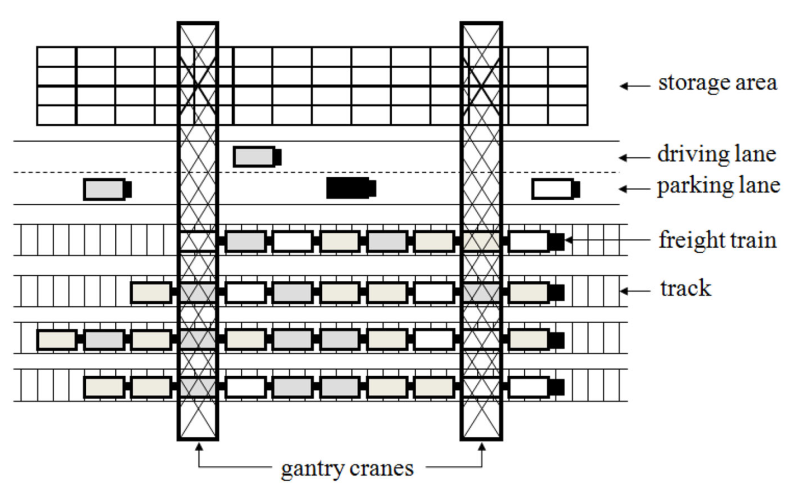
\includegraphics[width=\textwidth]{img/costs.png}
\caption{Schematische Darstellung eines Bahn-Terminals \cite{Briskorn2018}.}
\label{fig:costs}
\end{figure}
Die Transportkosten werden in einer Matrix $C = (c_{iq})_{n \times m}$ kodiert, \newline wobei $c_{iq} \coloneqq d_{man}(O_i, F_q)$.
D.h. der Eintrag an der Stelle $c_{iq}$ entspricht den Kosten für den Transport des \textit{Items} $i$ in den \textit{Stack} $q$.

%%%%%%%%%%%%%%%%%%%%%%%%%%%%%%%%%%%%%%%%%%%%%%%%%%%%%%%%%%%%%%%%%%%%%%%%%%%%%%%%%%%%%%%%%%%%%%%%%%%%
\pagebreak
%%%%%%%%%%%%%%%%%%%%%%%%%%%%%%%%%%%%%%%%%%%%%%%%%%%%%%%%%%%%%%%%%%%%%%%%%%%%%%%%%%%%%%%%%%%%%%%%%%%%

\subsection{Nebenbedingungen}
\label{sec:constraints}

\subsubsection{Stacking Restriktionen}
\label{sec:stacking_restrictions}

Es gibt in der Praxis vielfältige Gründe dafür, dass nicht jedes \textit{Item} auf jedes andere \textit{Item} gestapelt werden darf.
Aus diesen resultieren bestimmte Restriktionen, die z.B. wie folgt lauten:
\begin{itemize}
  \item schwerere \textit{Items} dürfen nicht auf leichteren \textit{Items} platziert werden
  \item größere \textit{Items} dürfen nicht auf kleineren \textit{Items} platziert werden
  \item \textit{Items} bestimmter Materialien oder Zielorte dürfen nicht aufeinander gestapelt werden
\end{itemize}

All jene Restriktionen, die im Folgenden stets als \textit{Stacking Constraints} bezeichnet werden, werden in einer Binärmatrix $S = (s_{ij})_{n \times n}$ kodiert, wobei:
\[
    s_{ij} =
\begin{cases}
    1, & \text{wenn $i$ direkt auf $j$ gestapelt werden darf }\\
    0, & \text{sonst}
\end{cases}
\]
Diese Matrix lässt sich, wie in Abb. \ref{fig:matrix_to_graph} beispielhaft dargestellt,
als gerichteter Graph mit $n$ Knoten für alle $i \in I$ und Kanten $i \rightarrow j$ für alle $s_{ij} = 1$ repräsentieren.
\begin{figure}[H]
  \begin{subfigure}[b]{0.5\textwidth}
  \centering
    $S =$
    $\left(
    \begin{array}{rrrr}
    0 & 1 & 1 & 0 \\
    1 & 0 & 1 & 0 \\
    1 & 0 & 0 & 0 \\
    1 & 1 & 1 & 0 \\
    \end{array} \right) $
    \caption{\textsc{Constraint Matrix}}
    \label{fig:constraint_matrix}
  \end{subfigure}
  \hfill
  \begin{subfigure}[b]{0.5\textwidth}
  \centering
    \begin{tikzpicture}[->, scale=0.50, transform shape, node distance=2.5cm]
    \node[state] (A) {1};
    \node[state] (B) [right of=A] {2};
    \node[state] (C) [below of=A] {3};
    \node[state] (D) [right of=C] {4};

    \path (A) edge node {} (B)
          (A) edge node {} (C)

          (B) edge [bend right] node {} (A)
          (B) edge [bend left=10] node {} (C)

          (C) edge [bend left] node {} (A)

          (D) edge [bend left=10] node {} (A)
          (D) edge node {} (B)
          (D) edge node {} (C);
  \end{tikzpicture}
    \caption{\textsc{Resultierender Graph}}
    \label{fig:resulting_graph}
  \end{subfigure}
  \caption{\textsc{Repräsentation der Stacking Constraints.}}
  \label{fig:matrix_to_graph}
\end{figure}
In dieser Arbeit werden ausschließlich transitive \textit{Stacking Constraints} betrachtet, d.h.
wenn \textit{Item} $i$ auf \textit{Item} $j$ und \textit{Item} $j$ auf \textit{Item} $h$ gestapelt werden darf,
so darf auch \textit{Item} $i$ auf \textit{Item} $h$ gestapelt werden.\newline
Diese Eigenschaft ist auch in der Praxis häufig gegeben.
Restriktionen bezüglich des Gewichts und der Länge haben die besondere Eigenschaft, dass alle Items vergleichbar sind, d.h. für alle $i \neq j  \quad \text{gilt} \quad s_{ij} = 1 \quad \text{oder} \quad s_{ji} = 1$, was bedeutet, dass diese Restriktionen eine totale Ordnung auf allen \textit{Items} definieren.

%%%%%%%%%%%%%%%%%%%%%%%%%%%%%%%%%%%%%%%%%%%%%%%%%%%%%%%%%%%%%%%%%%%%%%%%%%%%%%%%%%%%%%%%%%%%%%%%%%%%
\pagebreak
%%%%%%%%%%%%%%%%%%%%%%%%%%%%%%%%%%%%%%%%%%%%%%%%%%%%%%%%%%%%%%%%%%%%%%%%%%%%%%%%%%%%%%%%%%%%%%%%%%%%

\subsubsection{Placement Restriktionen}
\label{sec:placement_restrictions}

Die im Folgenden als \textit{Placement Constraints} bezeichneten Einschränkungen bezüglich der Position eines \textit{Items} resultieren z.B.
aus der Länge oder dem Gewicht der \textit{Items} und den Eigenschaften der \textit{Stacks}. Es gibt allerdings auch \textit{Items} mit speziellen Anforderungen, z.B. Kühlcontainer, die eine Energiequelle benötigen. Solche \textit{Items} können nur \textit{Stacks} mit entsprechender Konfiguration zugewiesen werden. Tendenziell sind dabei mehr \textit{Item}-\textit{Stack}-Zuweisungen erlaubt als verboten. Diese \textit{Placement Constraints} werden allerdings nicht direkt implementiert, sondern indirekt über hohe Kostenwerte.

Dies hat den Vorteil, dass die Placement Constraints zunächst nur \textquote{Weak Constraints} sind, d.h. es wird auch
dann eine Lösung gefunden, wenn gegen diese Nebenbedingungen verstoßen wird. Eine solche Lösung wird allerdings nur dann generiert,
wenn keine Lösung existiert, die sämtliche Placement Constraints respektiert.
Anschließend kann entschieden werden, ob solche Lösungen als zulässig gelten, oder, ob die Placement Constraints trotzdem
als \textquote{Hard Constraints} betrachtet und solche Lösungen dementsprechend unzulässig sind. Diese Art der Implementation ist sehr flexibel.

Der wesentliche Grund der Entscheidung für diese Art der Implementation ist allerdings eher pragmatischer Natur, denn der in den konstruktiven Heuristiken, die in Kapitel \ref{sec:constructive_heuristics} vorgestellt werden, verwendete Algorithmus zur Berechnung eines Minimum-Weight-Perfect-Matchings, erwartet einen vollständig bipartiten Graphen als Eingabe. Dies bedeutet, dass jedes Item zunächst mit jedem Stack kompatibel sein muss. Da die Placement Constraints genau dies jedoch verhindern, ist es sinnvoll, diese, wie im Folgenden beschrieben, indirekt über hohe Kostenwerte umzusetzen.

Zunächst werden die \textit{Placement Constraints} in einer Binärmatrix $T = (t_{iq})_{n \times m}$ kodiert, wobei:\newline
\[
    t_{iq} =
\begin{cases}
    1, & \text{wenn \textit{Item} $i$ in \textit{Stack} $q$ platziert werden darf }\\
    0, & \text{sonst}
\end{cases}
\]
Diese Matrix wird jedoch nicht direkt verwendet, um die Restriktionen zu implementieren. Stattdessen wird
die Transportkosten-Matrix $C = (c_{iq})_{n \times m}$, die in Abschnitt \ref{sec:transport_costs} eingeführt wurde, nun wie folgt erweitert.
\[
    c_{iq} =
\begin{cases}
    d_{man}(O_i, F_q), & \text{wenn $t_{iq} = 1$}\\
    \infty, & \text{sonst}
\end{cases}
\]
Der Eintrag an der Stelle $c_{iq}$ enthält also nur noch dann die tatsächlichen Transportkosten, wenn die
entsprechende \textit{Item}-\textit{Stack}-Zuweisung basierend auf den \textit{Placement Constraints} erlaubt ist und sonst $\infty$.

Die \textit{Placement Constraints} gelten als verletzt, wenn eine Lösung eine \textit{Item}-\textit{Stack}-Zuweisung der Kosten $\infty$ enthält.

%%%%%%%%%%%%%%%%%%%%%%%%%%%%%%%%%%%%%%%%%%%%%%%%%%%%%%%%%%%%%%%%%%%%%%%%%%%%%%%%%%%%%%%%%%%%%%%%%%%%
\pagebreak
%%%%%%%%%%%%%%%%%%%%%%%%%%%%%%%%%%%%%%%%%%%%%%%%%%%%%%%%%%%%%%%%%%%%%%%%%%%%%%%%%%%%%%%%%%%%%%%%%%%%

\subsection{Komplexität}
\label{sec:complexity}

In den folgenden Kapiteln werden Instanzen von Stacking Problemen mit den \textit{Stack}-Kapazitäten $b = 2$ und $b = 3 $ betrachtet,
die besonders in Szenarien aus der Praxis, in denen es darum geht, Container zu stapeln, von Interesse sind.

Wie \citet{Bruns2015} zeigten, handelt es sich bei dem Zulässigkeitsproblem mit einer \textit{Stack}-Kapazität von $b=3$ und gegebenen transitiven \textit{Stacking Constraints} $s_{ij}$ um ein stark NP-vollständiges Problem. Erst kürzlich wurde außerdem gezeigt, dass auch das Problem mit einer \textit{Stack}-Kapazität von $b=2$ mit gegebenen transitiven \textit{Stacking Constraints} $s_{ij}$ und \textit{Placement Constraints} $t_{iq}$ NP-vollständig ist. Diese Erkenntnis wurde allerdings noch nicht veröffentlicht. Somit sind auch die entsprechenden Stacking-Probleme, bei denen zusätzlich die Transportkosten minimiert werden, NP-vollständig. Für eben diese Probleme werden in dieser Arbeit heuristische Lösungsansätze präsentiert.

\subsection{Zielfunktion}
\label{sec:objective}

Das Ziel, welches im Folgenden für sämtliche Problemstellungen angestrebt wird, ist eine möglichst günstige
Einlagerung sämtlicher Items, d.h. die Zielfunktion entspricht der Minimierung der Transportkosten.
Dabei haben Zulässigkeit und geringe Laufzeit Priorität. Eine Lösung wird dann als zulässig betrachtet,
wenn sämtliche Items unter Berücksichtigung der Stacking- und Placement-Constraints sowie der Stack-Kapazität, eingelagert werden.

Der Fokus auf Zulässigkeit äußert sich darin, dass zunächst stets versucht wird, möglichst wenige der zur Verfügung stehenden Stacks zu verwenden, weshalb die Zielfunktion im Grunde zunächst darin besteht, die Anzahl der verwendeten Stacks zu minimieren bzw. die Anzahl der vollständig gefüllten Stacks zu maximieren, damit möglichst jede Instanz zumindest zulässig gelöst wird.

Erst im Anschluss daran werden die Transportkosten minimiert. Im Wesentlichen handelt es sich daher
um eine Kombination zweier Zielfunktionen. Zunächst geht es darum, den zur Verfügung stehenden Platz in
der Storage-Area durch initiales Generieren möglichst vieler $b$-Tupel von Items, möglichst ökonomisch zu nutzen.
Dabei werden noch keine Kosten minimiert. Anschließend geht es darum, diese $b$-Tupel möglichst günstig
den zur Verfügung stehenden Stacks zuzuweisen.

Ein ausschließlicher Fokus auf Kostenminimierung wäre umsetzbar, indem zuletzt ausgewählte $b$-Tupel
von Items wieder separiert und jeweils eigenen Stacks zugewiesen würden, solange freie Stacks zur Verfügung
stünden und sich infolgedessen Kosten einsparen ließen. Davon wird in dieser Arbeit abgesehen, da es in der Praxis durchaus sinnvoll ist, den zur Verfügung stehenden Platz möglichst ökonomisch zu nutzen und nicht bedingungslos Kosten zu minimieren und dabei viele lediglich partiell gefüllte Stacks zu generieren.

%%%%%%%%%%%%%%%%%%%%%%%%%%%%%%%%%%%%%%%%%%%%%%%%%%%%%%%%%%%%%%%%%%%%%%%%%%%%%%%%%%%%%%%%%%%%%%%%%%%%
\pagebreak
%%%%%%%%%%%%%%%%%%%%%%%%%%%%%%%%%%%%%%%%%%%%%%%%%%%%%%%%%%%%%%%%%%%%%%%%%%%%%%%%%%%%%%%%%%%%%%%%%%%%

\section{Testdaten-Generierung}
\label{sec:test_data}

Zu Testzwecken werden unterschiedlich große Instanzen von Stacking-Problemen generiert. Die Größe einer
Instanz bezieht sich dabei stets auf die Anzahl der betrachteten Items. Die Testinstanzen werden
in drei Kategorien unterteilt:
\begin{itemize}
  \item klein (\textbf{s}) ($\leq 100$ Items)
  \item mittelgroß (\textbf{m}) ($\approx 300$ Items)
  \item groß (\textbf{l}) ($\approx 500$ Items)\newline
\end{itemize}
Dies scheinen auch in der Literatur Größenordnungen zu sein, in dem sich praktisch motivierte Stacking-Probleme
typischerweise bewegen. \cite{Le2016}

Um die entwickelten Lösungsverfahren testen und vergleichen zu können, werden Testinstanzen generiert,
die im Idealfall nicht allzu weit von realistischen Szenarien entfernt sein sollten.
Pro Konfiguration werden 20 Instanzen generiert, damit aussagekräftige Ergebnisse entstehen.

\textbf{Anzahl zur Verfügung stehender Stacks}

Die Anzahl der \textit{Items} $n$ sowie die \textit{Stack}-Kapazität $b$ wird stets spezifiziert und in der Berechnung der Anzahl
zur Verfügung stehender \textit{Stacks} $m$ verwendet. Es gilt $m$ = $\ceil{\floor{\frac{n}{b}}$ + $20 \%}$.
Bei einer \textit{Stack}anzahl von $m$ = $\floor{\frac{n}{b}}$ gäbe es überhaupt keinen Spielraum bei der \textit{Item}platzierung. Aufgrund der in Abschnitt \ref{sec:constraints} geschilderten Nebenbedingungen wären die meisten Instanzen dann jedoch unlösbar.
Daher wurde zunächst ein durchaus geringer Spielraum von $20 \%$ eingeführt, der in weiteren Betrachtungen erhöht werden könnte.

\textbf{Stacking Constraints}

Es wurden zwei Varianten der \textit{Stacking-Constraint}-Generierung implementiert, die jeweils spezifische Vor- und Nachteile aufweisen.

\textbf{Variante 1}

Die \textit{Stacking-Constraint}-Matrix $S$ wird anhand einer definierten Wahrscheinlichkeit mit $1$- bzw. $0$-Einträgen gefüllt.
Anschließend werden die $1$-Einträge, die aus Transitivität folgen, ergänzt.

\textbf{Variante 2}

Für alle $n$ \textit{Items} wird eine zufällige Länge und Breite generiert. \textit{Item} $i$ kann auf \textit{Item} $j$ platziert werden,
wenn für dessen Länge $l_i$ und Breite $w_i$ gilt $l_i \leq l_j$ und $w_i \leq w_j$.
Zwei \textit{Items} $i, j$ sind in beide Richtungen stackbar, wenn $l_i = l_j$ und $w_i = w_j$ gilt.

Variante 2 scheint realitätsnäher zu sein und wird deshalb zunächst bevorzugt. Aufgrund der Tatsache, dass Variante 2 jedoch stets
zu einem Anteil von $1$-Einträgen in der Matrix von ca. $25\%$ führt und dieser mit Variante 1 sehr gut konfigurierbar ist, wird Variante 1 nicht verworfen. (TODO: Grund ergänzen...)

\textbf{Placement Constraints}

Die Placement Constraints werden zufällig generiert, wobei die Wahrscheinlichkeit für $t_{iq} = 1$, also dafür,
dass ein Item $i$ in einem Stack $q$ platziert werden darf, $70 \%$ beträgt, da, wie in Kapitel \ref{sec:placement_restrictions} bereits erwähnt, tendenziell mehr Zuweisungen erlaubt als verboten sind.

\textbf{Transportkosten}

Zur Transportkostenberechnung wird, wie in Abschnitt \ref{sec:transport_costs} erläutert, die Manhattan-Metrik verwendet. Dazu sind
entsprechend die \textit{Item}- und \textit{Stack}positionen als $x$- und $y$-Koordinaten gegeben. Auch die entsprechenden Längen und Breiten sowie die Distanz zwischen \textit{Storage-Area} und den Fahrzeug-Lanes ist jeweils gegeben.

%%%%%%%%%%%%%%%%%%%%%%%%%%%%%%%%%%%%%%%%%%%%%%%%%%%%%%%%%%%%%%%%%%%%%%%%%%%%%%%%%%%%%%%%%%%%%%%%%%%%
\pagebreak
%%%%%%%%%%%%%%%%%%%%%%%%%%%%%%%%%%%%%%%%%%%%%%%%%%%%%%%%%%%%%%%%%%%%%%%%%%%%%%%%%%%%%%%%%%%%%%%%%%%%

\section{MIP-Formulierungen}
\label{sec:mip_formulations}

In diesem Kapitel werden MIP-Formulierungen eingeführt, die dem experimentellen Vergleich dienen.
Diese werden verwendet, um die optimalen Zielfunktionswerte der Test-Instanzen zu ermitteln und somit eine Grundlage zu schaffen, mit der die Qualität der von den Heuristiken generierten Lösungen beurteilt werden kann. Des Weiteren geht es auch um einen Vergleich der im Folgenden vorgestellten MIP-Formulierungen untereinander. Zunächst wird in Abschnitt \ref{sec:mip_definition} kurz die Idee des MIP im Allgemeinen
eingeführt, um dann im Anschluss in den Abschnitten \ref{sec:bin_packing_formulation} und \ref{sec:three_idx_formulation} die beiden in dieser Arbeit betrachteten MIP-Formulierungen im Detail vorzustellen.

\subsection{Mixed Integer Linear Programming (MIP)}
\label{sec:mip_definition}

Viele kombinatorische Optimierungsprobleme lassen sich als lineare Programme formulieren, die sich dadurch
auszeichnen, dass die Zielfunktion eine lineare Funktion in Abhängigkeit von den Entscheidungsvariablen ist
und alle Nebenbedingungen in Form von linearen Gleichungen und Ungleichungen vorliegen. Für diese Probleme gibt es mit dem Simplexverfahren ein sehr effizientes Lösungsverfahren.\cite{Knust2017}

Ein gemischt-ganzzahliges lineares Programm (MIP) ist ein lineares Programm, welches kontinuierliche und ganzzahligen Variablen
enthält. Im Gegensatz zur kontinuierlichen Variante, ist die Lösung von ganzzahligen linearen Programmen NP-schwer.
Während sogar sehr große kontinuierliche lineare Programme durch kommerzielle Solver in wenigen Minuten gelöst werden können, gilt dies nicht für ganzzahlige lineare Programme. Diese können nur mit deutlich zeitaufwändigeren Algorithmen wie Branch \& Bound gelöst werden.\cite{Brucker2006}

In dieser Arbeit wird das Java-Interface von CPLEX, einem Solver für lineare Optimierungsprobleme verwendet,
um die MIP-Formulierungen, die in Abschnitt \ref{sec:bin_packing_formulation} und Abschnitt \ref{sec:three_idx_formulation} vorgestellt werden,
zu lösen. Es handelt sich dabei um eine unter anderem auf dem Simplexverfahren basierende Implementation von IBM. \cite{CPLEX2015}

\subsection{Bin-Packing-Formulierung}
\label{sec:bin_packing_formulation}

Die Bin-Packing-Formulierung orientiert sich dem Namen nach am klassichen \textsc{Bin-Packing} Problem, bei dem es darum geht,
eine Menge von Objekten so auf eine Menge von Behältern zu verteilen, dass die Behälterkapazitäten eingehalten werden.
Dies beschreibt auch direkt den Ansatz der Bin-Packing-Formulierung. Die Stacks werden als Behälter betrachtet und die Items als Objekte,
die diesen Behältern zugeordnet werden, wobei die Behälter- bzw. Stack-Kapazität jeweils eingehalten wird. Im Unterschied zum klassischen \textsc{Bin-Packing} müssen zusätzlich die Stacking- und Placement-Constraints berücksichtigt werden.

\pagebreak

Es sei eine Menge von Items $I = \{1, ..., n\}$ und eine Menge von Stacks $Q = \{1, ..., m\}$ mit einer Kapazität von $b$ gegeben.
Außerdem sei $G = (I, A)$ ein transitiver Stacking-Constraint-Graph, bei dem eine Kante $(i, j) \in A$ bedeutet,
dass die Items $i$ und $j$ in mindestens einer Richtung stackbar sind, also $s_{ij} = 1$ oder $s_{ji} = 1$.\newline
Bei den Variablen $x_{iq}$ handelt es sich um Binärvariablen, wobei $x_{iq} = 1$ bedeutet, dass Item $i$ Stack $q$ zugewiesen wird.
Die Kosten werden über die Variablen $c_{iq}$ modelliert, wobei $c_{iq}$ den Kosten für den Transport des Items $i$ in den Stack $q$
entspricht.

\begin{gather}
\boldsymbol{min} \quad \sum_{i \in I} \sum_{q \in Q} c_{iq} x_{iq} \label{bin_packing_line_one} \\
\thinspace\thinspace \boldsymbol{s.t.} \thinspace\quad\thinspace\thinspace\thinspace\quad\thinspace \quad \sum_{q \in Q} x_{iq} = 1 \quad\quad\quad\quad\quad\quad\quad \forall i \in I \quad\quad\quad\quad\thinspace\thinspace \label{bin_packing_line_two} \\
\quad \sum_{i \in I} x_{iq} \leq b \quad\quad\quad\quad\quad\quad\quad \forall q \in Q \label{bin_packing_line_three} \\
\thinspace\thinspace\quad\quad x_{iq} + x_{jq} \leq 1 \quad\quad\thinspace\thinspace\quad\quad\quad\quad \forall \{i, j\} \notin A \label{bin_packing_line_four} \\
\thinspace\thinspace\quad\quad\quad x_{iq} \in \{0, 1\} \thinspace\thinspace\thinspace\thinspace\thinspace\thinspace\quad\quad\quad\quad\quad\quad \forall i \in I, q \in Q \thinspace \label{bin_packing_line_five}
\end{gather}

In (\ref{bin_packing_line_one}) wird die betrachtete Zielfunktion definiert, welche die Summe der Kosten sämtlicher
Item-Stack-Zuweisungen minimiert, was der Minimierung der Transportkosten entspricht.
Nebenbedingung (\ref{bin_packing_line_two}) fordert, dass jedes Item genau einem Stack zugewiesen wird. Die Ungleichung in (\ref{bin_packing_line_three}) entspricht der Forderung, dass für sämtliche Stacks die Stack-Kapazität eingehalten werden muss, d.h.
die Summe der eines Stacks zugewiesenen Items darf dessen Kapazität nicht überschreiten. (\ref{bin_packing_line_four}) entspricht schließlich der Forderung, dass alle Items, die nicht stackbar sind, für die also keine Kante im Stacking-Constraint-Graph existiert, nicht Teil desselben Stacks sind. Außerdem handelt es sich laut (\ref{bin_packing_line_five}), wie bereits erwähnt, bei den Variablen $x_{iq}$ um Binärvariablen.

\subsection{3-Index-Formulierung}
\label{sec:three_idx_formulation}

Die 3-Index-Formulierung enthält drei Indizes - Item, Stack und Level.
Im Gegensatz zur Bin-Packing-Formulierung, die Item-Stack-Zuweisungen vornimmt, weist die 3-Index-Formulierung einem
Item auch eine konkrete Position innerhalb eines Stacks zu, sie berücksichtigt also den Level.

Gegeben sei erneut eine Item-Menge $I = \{1, ..., n\}$ und eine Stack-Menge $Q = \{1, ..., m\}$, die Stacks der Kapazität $b$ enthält.
Jeder Stack enthält dementsprechend die Level $L = \{1, ..., b\}$. Des Weiteren sei ein transitiver Stacking-Constraint-Graph
$G = (I, A)$ gegeben, bei dem eine Kante $i \rightarrow j \in A$ bedeutet, dass das Item $i$ direkt auf das Item $j$ gestapelt werden darf.
Die Kosten seien durch die gegebene Transportkostenmatrix $C$ definiert, in der an der Stelle $c_{iq}$ die Kosten für den
Transport von Item $i$ in Stack $q$ stehen. Bei den Variablen $x_{iql}$ handelt es sich um Binärvariablen,
bei denen $x_{iql} = 1$ bedeutet, dass Item $i$ in Stack $q$ auf Level $l$ platziert wird.

\begin{gather}
\boldsymbol{min} \quad \sum_{i \in I} \sum_{q \in Q} \sum_{l \in L} c_{iq} x_{iql} \label{three_idx_line_one} \\
\boldsymbol{s.t.} \quad \sum_{q \in Q} \sum_{l \in L} x_{iql} = 1 \quad\thinspace\thinspace\quad\quad\quad\quad \forall i \in I \thinspace\thinspace\quad\quad\quad\quad\quad\quad\quad\quad\thinspace\thinspace \label{three_idx_line_two} \\
\sum_{i \in I} x_{iql} \leq 1 \thinspace\quad\quad\quad\quad\quad\quad\quad \forall q \in Q, l \in L \thinspace\thinspace\thinspace\thinspace\quad\quad\quad\thinspace \label{three_idx_line_three} \\
\sum_{j \in I | i \rightarrow j \in A} x_{jq(l-1)} - x_{iql} \geq 0 \thinspace\quad\quad \forall i \in I, q \in Q, l \in L \textbackslash \{1\}
\label{three_idx_line_four} \\
\quad\quad x_{iql} \in \{0, 1\} \quad\quad\quad\quad\quad\quad\quad \forall i \in I, q \in Q, l \in L \quad\thinspace\thinspace\thinspace\thinspace\thinspace \label{three_idx_line_five}
\end{gather}

In (\ref{three_idx_line_one}) wird die Zielfunktion definiert, die erneut die Summe der Kosten sämtlicher Item-Zuweisungen
und somit die Transportkosten minimiert.
Nebenbedingung (\ref{three_idx_line_two}) fordert, dass sich jedes Item in genau einem Stack an genau einer Position (Level) befindet.
Anschließend wird in (\ref{three_idx_line_three}) gefordert, dass sich an jeder Position in jedem Stack höchstens ein Item befindet und
(\ref{three_idx_line_four}) formuliert die Einschränkung, dass jedes Item, welches oberhalb des Ground-Levels platziert wird,
ein Item unter sich hat, welches sich basierend auf den Stacking Constraints dort befinden darf. Schließlich wird in (\ref{three_idx_line_five}) festgehalten, dass es sich bei den $x_{iql}$ um Binärvariablen handelt.

Beide Formulierungen weisen jedem Item einen Stack zu und minimieren dabei die Transportkosten.
Die Bin-Packing-Formulierung nimmt dabei lediglich Item-Stack-Zuweisungen vor, während die 3-Index-Formulierung die
Items konkreten Positionen innerhalb der Stacks zuweist. Dabei ist allerdings auch bei der Bin-Packing-Formulierung
sichergestellt, dass eine Item-Stack-Zuweisung nur dann vorgenommen wird, wenn die Items innerhalb des Stacks anschließend
in einer Weise umsortiert werden können, dass sie den Stacking Constraints entsprechen. Diese Tatsache ergibt sich aus Nebenbedingung (\ref{bin_packing_line_four}), welche fordert, dass Items sich nur dann im selben Stack befinden, wenn sie in mindestens einer Richtung stackbar sind.
Da die Stacking Constraints außerdem transitiv sind, ist sichergestellt, dass die Reihenfolge innerhalb der Stacks stets so korrigiert
werden kann, dass eine valide Lösung, die die Stacking Constraints respektiert, dabei herauskommt.

Die 3-Index-Formulierung liefert folglich direkt eine zulässige Lösung, während die Item-Stack-Zuweisungen, die die Bin-Packing-Formulierung liefert, zunächst noch sortiert werden müssen, damit sie eine zulässige Lösung ergeben. Dies kann durch den simplen Algorithmus \ref{alg:algo1} erreicht werden.

% \begin{algorithm}
% \fontsize{10pt}{10pt}

% \SetAlgoLined

%   \ForEach{stack in storageArea}{

%     somethingChanged = true\;

%     \While{somethingChanged}{

%       somethingChanged = false\;

%       \For{position = 0; position < stack.capacity - 1; position++}{
%           \BlankLine\BlankLine
%           \uIf{stack[position].\Call{isOccupied()}{} \&\& stack[position + 1].\Call{isOccupied()}{{}}}{
%             \uIf{itemAt(stack[position]).\Call{isStackableOn}{itemAt(stack[position + 1])}}{

%                 \Call{exchangeItems}{stack[position], stack[position + 1]}\;
%                 somethingChanged = true\;
%                 break\;
%             }
%           }
%       }
%     }
%   }

% \caption{Korrektur der Item Reihenfolge innerhalb der Stacks.}
% \label{alg:algo1}
% \end{algorithm}

%%%%%%%%%%%%%%%%%%%%%%%%%%%%%%%%%%%%%%%%%%%%%%%%%%%%%%%%%%%%%%%%%%%%%%%%%%%%%%%%%%%%%%%%%%%%%%%%%%%%
\pagebreak
%%%%%%%%%%%%%%%%%%%%%%%%%%%%%%%%%%%%%%%%%%%%%%%%%%%%%%%%%%%%%%%%%%%%%%%%%%%%%%%%%%%%%%%%%%%%%%%%%%%%

\section{Konstruktive Heuristiken}
\label{sec:constructive_heuristics}

Bei den entwickelten konstruktiven Heuristiken handelt es sich um effiziente Lösungsverfaren für die in Kapitel \ref{sec:stacking_problems}
beschriebenen Problemstellungen. Zunächst werden drei wichtige Konzepte eingeführt, welche in den Heuristiken Verwendung finden.
In \ref{sec:digression_bipartite_graph} bipartite Graphen, in \ref{sec:digression_mwpm} Minimum-Weight-Perfect-Matchings und in \ref{sec:digression_mcm} Maximum-Cardinality-Matchings. Anschließend geht es in \ref{sec:two_cap_heuristic} um die konstruktive Heuristik
für eine Stack-Kapazität von $b=2$ und darauffolgend in \ref{sec:solver_comp_b=2} um einen experimentellen Vergleich der Solver für
eben diese Stack-Kapazität in Bezug auf die benötigten Laufzeiten und die Qualität der generierten Lösungen.
Abschnitt \ref{sec:three_cap_heuristic} behandelt die konstruktive Heuristik für eine Stack-Kapazität von $b=3$, worauf erneut ein Vergleich der entsprechenden Solver in \ref{sec:solver_comp_b=3} folgt.

\subsection{Hintergrund}

\subsubsection{Bipartiter Graph}
\label{sec:digression_bipartite_graph}

Ein Graph $G = (V, E)$ heißt bipartit (vgl. Abb. \ref{fig:digression_bipartite_graph}), wenn die Knotenmenge in zwei disjunkte Teilmengen zerfällt
$(V = S \cup T$ mit $S \cap T = \emptyset$), sodass jede Kante einen Knoten aus $S$ mit einem Knoten aus $T$ verbindet. \cite{HochschuleDarmstadt}\newline
Es lassen sich folgende Äquivalenzen festhalten \cite{Leighton2010}:
\begin{itemize}
  \item $G$ bipartit $\iff$ $G$ 2-färbbar
  \item $G$ bipartit $\iff$ keine Kreise ungerader Länge in $G$
\end{itemize}
In Abb. \ref{fig:digression_bipartite_graph} ist die 2-Färbbarkeit eines bipartiten Graphen, bei welcher die eine Teilmenge
in grün und die andere Teilmenge in rot gefärbt ist, visualisiert. Wie man sieht, existieren in solchen Graphen
ausschließlich Kanten, welche einen Knoten der einen Teilmenge (rot) mit einem Knoten der anderen Teilmenge (grün) verbinden,
jedoch keine Kanten zwischen Knoten derselben Farbe bzw. Teilmenge.

\begin{figure}[H]
\centering
\begin{tikzpicture}[scale=0.6, transform shape, node distance=3cm]
  \node[state] [green] (A) {};
  \node[state] [red] (B) [above right of=A] {};
  \node[state] [green] (C) [below right of=B] {};
  \node[state] [red] (D) [below of=B] {};
  \node[state] [red] (E) [below of=A] {};
  \node[state] [green] (F) [right of=E] {};

  \path (A) edge node {} (B)
        (B) edge node {} (C)
        (C) edge node {} (D)
        (A) edge node {} (D)
        (A) edge node {} (E)
        (E) edge node {} (F)
        (D) edge node {} (F);

\end{tikzpicture}
\caption{\textsc{Bipartiter Graph.}}
\label{fig:digression_bipartite_graph}
\end{figure}

Ein Graph wird als vollständig bipartit bezeichnet, wenn jeder Knoten der einen Teilmenge mit jedem Knoten
der anderen Teilmenge durch eine Kante verbunden ist. Der in Abb. \ref{fig:digression_bipartite_graph}
dargestellte Graph ist dementsprechend nicht vollständig bipartit.

\subsubsection{Minimum-Weight-Perfect-Matching (\textsc{MWPM})}
\label{sec:digression_mwpm}

Gegeben sei ein ungerichteter Graph $G = (V, E)$. Eine Menge $M \subseteq E$ heißt Matching,
wenn keine zwei Kanten aus $M$ einen Knoten gemeinsam haben. Bei einem Matching handelt es sich also
um eine Menge unabhängiger Kanten. Ein Perfect-Matching ist wiederum ein Matching, welches sämtliche Knoten des Graphen enthält.
Jeder Knoten des Graphen ist dabei inzident zu genau einer Kante des Matchings (vgl. Abb. \ref{fig:perfect_matching}).
Daher ist ein Perfect-Matching nur für Graphen mit einer geraden Anzahl an Knoten möglich.
Ein Minimum-Weight-Perfect-Matching ist ein günstigstes Perfect-Matching basierend auf den Kantenkosten.
\begin{figure}[H]
\centering
\begin{tikzpicture}[-, scale=0.6, transform shape, node distance=3cm]
    \node[state] (A) {};
    \node[state] (B) [above right of=A] {};
    \node[state] (C) [below right of=A] {};
    \node[state] (D) [right of=B] {};
    \node[state] (E) [right of=D] {};
    \node[state] (F) [right of=C] {};

    \path (A) edge [red] node {} (B)
          (A) edge node {} (C)
          (B) edge node {} (D)
          (B) edge node {} (C)
          (D) edge [red] node {} (E)
          (D) edge node {} (F)
          (C) edge [red] node {} (F);
\end{tikzpicture}
\caption{\textsc{Perfect-Matching (dargestellt in rot).}}
\label{fig:perfect_matching}
\end{figure}

Der Algorithmus zur Berechnung von Minimum-Weight-Perfect-Matchings, welcher in den im Folgenden
vorgestellten Heuristiken zum Einsatz kommt, stammt aus der Java-Bibliothek \textit{JGraphT} \cite{JGraphT}, trägt
den Namen \textit{KuhnMunkresMinimalWeightBipartitePerfectMatching} und ist eine Implementation der
sogenannten Ungarischen Methode zum Lösen von Zuordnungsproblemen in bipartiten Graphen.
Die Laufzeitkomplexität der Implementation beträgt $O(n^3)$, wobei $n$ der Anzahl der Knoten im Graphen entspricht.
Als Eingabe wird ein vollständig bipartiter Graph $G$ erwartet, d.h. $G= (S \cup T, E)$, wobei $S \cap T = \emptyset$ und
$\forall s \in S, t \in T \thinspace \exists \thinspace \{s, t\} \in E$. Außerdem wird erwartet, dass beide Partitionen gleich groß sind,
also $|S| = |T|$. Bei der Rückgabe des Algorithmus handelt es sich um ein Perfect-Matching der geringsten Kosten.

\subsubsection{Maximum-Cardinality-Matching (MCM)}
\label{sec:digression_mcm}

Sei $M$ ein Matching in einem Graphen $G$. Falls $M$ als Menge eine maximale Kardinalität unter
allen Matchings von $G$ hat, wird dies als Maximum-Cardinality-Matching bezeichnet. \cite{WikiMatching}
Es kann mehrere unterschiedliche MCMs in einem Graphen geben.
In Abb. \ref{fig:mcm_examples} sind beispielhaft zwei MCMs dargestellt.
\begin{figure}[H]
  \begin{subfigure}[b]{0.4\textwidth}
  \centering
    \begin{tikzpicture}[scale=0.55, transform shape, node distance=2cm]
    \node[state] (A) {};
    \node[state] (B) [above right of=A] {};
    \node[state] (C) [below left of=A] {};
    \node[state] (D) [below right of=C] {};
    \node[state] (F) [below right of=B] {};
    \node[state] (E) [below of=F] {};

    \path (A) edge [red] node {} (B)
          (A) edge node {} (C)
          (A) edge node {} (D)
          (A) edge node {} (E)
          (A) edge node {} (F)
          (C) edge [red] node {} (D);
  \end{tikzpicture}
  \caption{\textsc{$|MCM| = 2$}}
  \label{fig:mcm1}
  \end{subfigure}
  \hfill
  \begin{subfigure}[b]{0.4\textwidth}
  \centering
    \begin{tikzpicture}[scale=0.55, transform shape, node distance=2cm]
    \node[state] (A) {};
    \node[state] (B) [right of=A] {};
    \node[state] (C) [right of=B] {};
    \node[state] (D) [below left of=A] {};
    \node[state] (E) [below right of=D] {};
    \node[state] (F) [right of=E] {};

    \path (A) edge node {} (B)
          (B) edge [red] node {} (C)
          (B) edge node {} (F)
          (A) edge node {} (E)
          (E) edge [red] node {} (F)
          (A) edge [red] node {} (D)
          (D) edge node {} (E);
  \end{tikzpicture}
    \caption{\textsc{$|MCM| = 3$}}
    \label{fig:mcm_2}
  \end{subfigure}
  \caption{\textsc{MCMs (dargestellt in rot).}}
  \label{fig:mcm_examples}
\end{figure}

Der Algorithmus zur Berechnung von Maximum-Cardinality-Matchings, welcher in den im Folgenden
vorgestellten Heuristiken Anwendung findet, stammt ebenfalls aus der Java-Bibliothek \textit{JGraphT} \cite{JGraphT} und trägt
den Namen \textit{EdmondsMaximumCardinalityMatching}. Es handelt sich dabei um eine Implementation von Edmonds' Blossom-Algorithmus,
welcher MCMs in ungerichteten Graphen berechnet. Der Algorithmus liefert ein Perfect-Matching, sofern eines existiert.
Andernfalls wird das größte Non-Perfect-Matching zurückgegeben.
Der Algorithmus besitzt eine Laufzeitkomplexität von $O(nm \thinspace \alpha(m, n))$. Wobei $n$ der Anzahl der Knoten
und $m$ der Anzahl der Kanten im Graphen entspricht. Im \textquote{Average-Case}, also im Regelfall, ist der Algorithmus jedoch effizienter.

\subsection{Konstruktive Heuristik ($b = 2$)}
\label{sec:two_cap_heuristic}

Die konstruktive Heuristik zur Lösung von Stacking-Problemen mit Stacks der Kapazität $b=2$ erweitert den Ansatz aus dem Beweis
zu Theorem 1 aus der einleitend erwähnten Arbeit von \citet{Bruns2015}.

Zunächst wird ein Stacking-Constraint-Graph $G = (V, E)$ generiert, welcher die Items als Knoten enthält, d.h. $V = I$. Dieser Graph
enthält eine Kante $\{i, j\} \in E$ zwischen zwei Knoten, wenn die entsprechenden Items $i, j \in I$ basierend auf den Stacking-Constraints
in mindestens einer Richtung stackbar sind, d.h. wenn $s_{ij} + s_{ji} \geq 1$ und wenn mindestens ein Stack existiert, in welchem die beiden Items gemeinsam platziert werden können ohne die Placement-Constraints zu verletzen, also wenn $c_{iq} < \infty$ und $c_{jq} < \infty$ für
mindestens einen Stack $q \in Q$ gilt.

Berechnet man nun ein \textsc{MCM} in $G$ und interpretiert dessen Kanten als Stacks, welche die beiden Knoten, die durch
die Kanten verbunden werden, als Items enthalten, so erhält man eine größtmögliche Anzahl an vollständig gefüllten Stacks.
Items, welche nicht inzident zu einer Kante des Matchings sind, werden auf dem Ground-Level eines eigenen Stacks platziert.
Insgesamt werden auf diese Weise so wenig Stacks wie möglich verwendet, denn auch wenn der eigentliche Gegenstand der Optimierung die Transportkosten sind, steht zunächst stets im Vordergrund, überhaupt eine zulässige Lösung zu finden, weshalb die Maximierung der Anzahl der vollständig gefüllten Stacks initial eine gute Strategie darstellt.
Eine zulässige Lösung mit maximal $m$ Stacks kann nur dann existieren, wenn die Anzahl der Kanten im Matching und die Anzahl der nicht gematchten Knoten in der Summe nicht größer ist als $m$.

Aufgrund der Placement-Constraints kann allerdings nicht jedes Item in jedem Stack platziert werden, weshalb noch die bestmögliche Zuweisung von
Items und Item-Paaren zu Stacks gefunden werden muss. Diese entspricht einer Zuweisung, in welcher sämtliche Items möglichst günstig einem
kompatiblen Stack zugeordnet werden. Dazu wird ein bipartiter Graph $G_1 = (V_1 \cup V_2, A)$ eingeführt, dessen erste Partition $V_1$ die Items bestehend aus Item-Paaren und Unmatched-Items enthält während die zweite Partition $V_2$ die zur Verfügung stehenden Stacks beinhaltet.
Eine Kante $\{i, q\} \in A$ zwischen einem Knoten $i \in V_1$ und einem Knoten $q \in V_2$ gibt an, dass das entsprechende Item oder Item-Paar $i$ dem jeweiligen Stack $q$ zugeordnet werden kann. Da die Placement-Constraints nicht direkt durch ein Fehlen der entsprechenden Kante in $G_1$, sondern indirekt durch ein hohes Gewicht ebendieser Kante umgesetzt werden, existieren Kanten zwischen sämtlichen Knoten
aus $V_1$ und denen aus $V_2$, also $\forall i \in V_1, q \in V_2 \thinspace \exists \thinspace \{i, q\} \in A$.
Das Gewicht einer solchen Kante ist definiert als die Kosten $c_{iq}$ des Transports des Items $i$ von seiner Originalposition $O_i$ auf dem Fahrzeug, mit welchem es geliefert wird, zum Stack $q$
in der Storage-Area. Im Fall eines Item-Paars $(i, j) \in V_1$ entspricht das
Gewicht der Kante $\{(i, j), q\} \in A$ der Summe der Kosten des Transports beider Items, also $c_{(i, j)q} = c_{iq} + c_{jq}$.

Da der von \textit{JGraphT} bereitgestellte Algorithmus, welcher zur Berechnung eines \textsc{MWPM} in $G_1$ verwendet wird,
einen vollständig bipartiten Graphen, dessen Partitionen dieselbe Größe besitzen, als Eingabe erwartet und die Summe der Items und Item-Paare
nicht notwendigerweise der Anzahl der verfügbaren Stacks entspricht, werden Dummy-Items eingeführt.
Diese Dummy-Items füllen $V_1$ für den Fall, dass diese Partition kleiner ist, auf.
Übersteigt die Anzahl der Items und Item-Paare die Anzahl der zur Verfügung stehenden Stacks, so existiert,
wie bereits erwähnt, ohnehin keine zulässige Lösung.

Die Dummy-Items haben keinen Einfluss auf die Lösung, da sämtliche Kanten, die ein Dummy-Item mit einem Stack verbinden,
das Gewicht $0$ besitzen und somit keine günstigere Zuweisung eines echten Items oder Item-Paars durch ein Dummy-Item
verhindert wird. Diese Tatsache ergibt sich daraus, dass die Dummy-Items jedem Stack zu den Kosten $0$ zugewiesen
werden können, während eine Zuweisung echter Items und Item-Paare stets Kosten verursacht. Dementsprechend werden
echte Items bei der Zuweisung gewissermaßen bevorzugt während Dummy-Items schlicht den verbleibenden Stacks zugewiesen werden.

Nachdem beide Partitionen dieselbe Größe besitzen, wird ein \textsc{MWPM} in $G_1$ berechnet, dessen Kanten als
Stackzuweisungen interpretiert werden. Da es sich um ein Perfect-Matching handelt, werden sämtliche Items und Item-Paare einem Stack zugewiesen. Die Minimum-Weight-Variante eines Perfect-Matchings sorgt dafür, dass es sich um eine günstigste Zuweisung sämtlicher Items und Item-Paare zu Stacks handelt, da die Kantenkosten jeweils den Transportkosten der entsprechenden Items entsprechen. Sollte das \textsc{MWPM} eine Kante der Kosten $\infty$ enthalten, so existiert keine zulässige Zuweisung der generierten Item-Paare und Unmatched Items zu den Stacks, welche die Placement-Constraints respektiert.

Abschließend muss ggf. die Reihenfolge der Items innerhalb der Stacks angepasst werden, da für die Item-Paare bisher nur sichergestellt ist,
dass sie kompatibel und somit in mindestens einer Richtung stackbar sind. Die Richtung, in welcher sie stackbar sind, wurde bei der Zuweisung
jedoch noch nicht berücksichtigt. Dies ist trivial möglich, indem für jene Stacks, welche ein Item-Paar beinhalten,
überprüft wird, ob die Stacking-Constraints respektiert werden. Ist dies nicht der Fall, so werden die Items vertauscht.
Anschließend ist garantiert, dass sämtliche Paare den Stacking-Constraints genügen.

\pagebreak

\textbf{Beispiel}

Gegeben sei die Item-Menge $I = \{0, 1, 2, 3, 4, 5, 6\}$ sowie eine Stack-Kapazität von $b = 2$.
Die Anzahl der zur Verfügung stehenden Stacks wird nun, wie in Abschnitt \ref{sec:test_data} geschildert,
durch $m = \ceil{\floor{\frac{n}{b}} + 20 \%}$ berechnet und entspricht somit $m = \ceil{\floor{\frac{7}{2}} + 20 \%} = 4$.
Die Stacking-Constraint-Matrix $S$ wird ebenfalls, wie in Abschnitt \ref{sec:test_data} beschrieben, generiert.
Basierend auf dieser wird der in Abb. \ref{fig:stacking_const_graph_example_b=2_a} dargestellte Stacking-Constraint-Graph
für die gegebenen Items eingeführt, auf welchem anschließend das in Abb. \ref{fig:stacking_const_graph_example_b=2_b} in grün dargestellte \textsc{MCM} berechnet wird. Das in rot dargestellte Item $0$ verbleibt dabei als einziges Unmatched-Item.
\begin{figure}[H]
  \centering
    \begin{subfigure}[b]{0.4\textwidth}
    \centering
    \begin{tikzpicture}[scale=0.75, transform shape, node distance=3cm]
        \node[state] (G) [thick] {$\boldsymbol{6}$};
        \node[state] (B) [thick, above left of=G] {$\boldsymbol{1}$};
        \node[state] (C) [thick, above right of=G] {$\boldsymbol{2}$};
        \node[state] (E) [thick, below right of=G] {$\boldsymbol{4}$};
        \node[state] (F) [thick, below left of=G] {$\boldsymbol{5}$};
        \node[state] (A) [thick, below left of=B] {$\boldsymbol{0}$};
        \node[state] (D) [thick, below right of=C] {$\boldsymbol{3}$};

        \path (B) edge [thick] node {} (C)
              (B) edge [thick] node {} (F)
              (B) edge [thick] node {} (G)
              (C) edge [thick, bend right = 75, distance=5cm] node {} (F)
              (C) edge [thick] node {} (E)
              (C) edge [thick] node {} (D)
              (C) edge [thick] node {} (G)
              (F) edge [thick] node {} (G)
              (F) edge [thick] node {} (E)
              (E) edge [thick] node {} (G);
    \end{tikzpicture}
    \caption{\textsc{Stacking-Constraint-Graph}}
    \label{fig:stacking_const_graph_example_b=2_a}
    \end{subfigure}
    \hfill
    \begin{subfigure}[b]{0.4\textwidth}
    \centering
    \begin{tikzpicture}[scale=0.75, transform shape, node distance=3cm]
        \node[state] (G) [thick] {$\boldsymbol{\textcolor{mygreen}{6}}$};
        \node[state] (B) [thick, above left of=G] {$\boldsymbol{\textcolor{mygreen}{1}}$};
        \node[state] (C) [thick, above right of=G] {$\boldsymbol{\textcolor{mygreen}{2}}$};
        \node[state] (E) [thick, below right of=G] {$\boldsymbol{\textcolor{mygreen}{4}}$};
        \node[state] (F) [thick, below left of=G] {$\boldsymbol{\textcolor{mygreen}{5}}$};
        \node[state] (A) [thick, below left of=B] {$\boldsymbol{\textcolor{red}{0}}$};
        \node[state] (D) [thick, below right of=C] {$\boldsymbol{\textcolor{mygreen}{3}}$};

        \path (B) edge [thick] node {} (C)
              (B) edge [thick] node {} (F)
              (B) edge [thick, mygreen] node {} (G)
              (C) edge [thick, bend right = 75, distance=5cm] node {} (F)
              (C) edge [thick] node {} (E)
              (C) edge [thick, mygreen] node {} (D)
              (C) edge [thick] node {} (G)
              (F) edge [thick] node {} (G)
              (F) edge [thick, mygreen] node {} (E)
              (E) edge [thick] node {} (G);
    \end{tikzpicture}
    \caption{\textsc{MCM (Item $0$ unmatched)}}
    \label{fig:stacking_const_graph_example_b=2_b}
    \end{subfigure}
\caption{\textsc{Generierung der Item-Paare}.}
\label{fig:stacking_const_graph_example_b=2}
\end{figure}
Die Kanten des in Abb. \ref{fig:stacking_const_graph_example_b=2_b} in grün dargestellten \textsc{MCM} werden nun,
wie in Abb. \ref{fig:item_pairs_b=2} dargestellt, als kompatible Item-Paare interpretiert. Das als unmatched verbleibende
Item $0$ wird im Folgenden dem Ground-Level eines eigenen Stacks zugewiesen.
\begin{figure}[H]
\centering
\begin{tikzpicture}[scale=0.7, transform shape, node distance=3cm]
        \node[state] (A) [thick] {\textcolor{mygreen}{$\boldsymbol{1, 6}$}};
        \node[state] (B) [thick, right of=A] {\textcolor{mygreen}{$\boldsymbol{2, 3}$}};
        \node[state] (C) [thick, right of=B] {\textcolor{mygreen}{$\boldsymbol{4, 5}$}};
        \node[state] (D) [thick, right of=C] {\textcolor{red}{$\boldsymbol{0}$}};
        \path ;
  \end{tikzpicture}
  \caption{\textsc{Resultierende Item-Paare.}}
  \label{fig:item_pairs_b=2}
\end{figure}

Nun geht es darum, eine möglichst günstige Zuweisung der Item-Paare und Unmatched-Items zu Stacks zu finden,
welche die Placement-Constraints respektiert. Dazu wird zunächst der vollständig bipartite Graph, welcher in
Abb. \ref{fig:bipartite_graph} dargestellt ist, generiert. Dieser enthält die Items bestehend aus Item-Paaren
und Unmatched-Items in der einen Partition und die Stacks in der anderen. Da bereits beide Partitionen
dieselbe Größe besitzen, müssen in diesem Fall keine Dummy-Items eingeführt werden.

Anschließend wird im bipartiten Graphen aus Abb. \ref{fig:bipartite_graph} das \textsc{MWPM} berechnet,
welches in Abb. \ref{fig:mwpm_b=2} dargestellt ist. Jede Kante entspricht dabei der Zuweisung eines Item-Paars bzw. Unmatched-Items
zu einem Stack.

\begin{figure}[H]
\begin{subfigure}[b]{0.5\textwidth}
\centering
\begin{tikzpicture}[scale=0.7, transform shape, node distance=1.5cm]
        \node[state] (A) [thick] {$\boldsymbol{1, 6}$};
        \node[state] (B) [thick, below of=A] {$\boldsymbol{2, 3}$};
        \node[state] (C) [thick, below of=B] {$\boldsymbol{4, 5}$};
        \node[state] (D) [thick, below of=C] {$\boldsymbol{0}$};

        \node[state] (F) [thick, right = 4cm of A] {$\boldsymbol{S_1}$};
        \node[state] (G) [thick, right = 4cm of B] {$\boldsymbol{S_2}$};
        \node[state] (H) [thick, right = 4cm of C] {$\boldsymbol{S_3}$};
        \node[state] (I) [thick, right = 4cm of D] {$\boldsymbol{S_4}$};

        \path
          % from (1,6) to all stacks
          (A) edge [thick] node {} (F)
          (A) edge [thick] node {} (G)
          (A) edge [thick] node {} (H)
          (A) edge [thick] node {} (I)

          % from (2,3) to all stacks
          (B) edge [thick] node {} (F)
          (B) edge [thick] node {} (G)
          (B) edge [thick] node {} (H)
          (B) edge [thick] node {} (I)

          % from (4,5) to all stacks
          (C) edge [thick] node {} (F)
          (C) edge [thick] node {} (G)
          (C) edge [thick] node {} (H)
          (C) edge [thick] node {} (I)

          % from 0 to all stacks
          (D) edge [thick] node {} (F)
          (D) edge [thick] node {} (G)
          (D) edge [thick] node {} (H)
          (D) edge [thick] node {} (I);
  \end{tikzpicture}
  \caption{\textsc{Vollständig bipartiter Graph}.}
  \label{fig:bipartite_graph}
\end{subfigure}
\hfill
\begin{subfigure}[b]{0.5\textwidth}
\centering
\begin{tikzpicture}[scale=0.7, transform shape, node distance=1.5cm]
        \node[state] (A) [thick] {$\boldsymbol{1, 6}$};
        \node[state] (B) [thick, below of=A] {$\boldsymbol{2, 3}$};
        \node[state] (C) [thick, below of=B] {$\boldsymbol{4, 5}$};
        \node[state] (D) [thick, below of=C] {$\boldsymbol{0}$};

        \node[state] (F) [thick, right = 4cm of A] {$\boldsymbol{S_1}$};
        \node[state] (G) [thick, right = 4cm of B] {$\boldsymbol{S_2}$};
        \node[state] (H) [thick, right = 4cm of C] {$\boldsymbol{S_3}$};
        \node[state] (I) [thick, right = 4cm of D] {$\boldsymbol{S_4}$};

        \path
          (A) edge [thick] node {} (I)
          (B) edge [thick] node {} (H)
          (C) edge [thick] node {} (G)
          (D) edge [thick] node {} (F);
  \end{tikzpicture}
  \caption{\textsc{MWPM}}
  \label{fig:mwpm_b=2}
\end{subfigure}
\caption{\textsc{Generierung der Stack-Zuweisungen}.}
\end{figure}

Sofern das in Abb. \ref{fig:mwpm_b=2} dargestellte \textsc{MWPM} keine Kante der Kosten $\infty$
enthält, handelt es sich um eine günstigste, zulässige Zuweisung sämtlicher Items und Item-Paare
zu Stacks. Andernfalls existiert keine solche Zuweisung für die gegebenen Paare und Unmatched-Items.
Die entsprechende Interpretation des \textsc{MWPM} als zulässige Stack-Zuweisungen ist in Abb.
\ref{fig:stacking_solution} visualisiert.

\begin{figure}[H]
  \centering
  \resizebox{0.35\textwidth}{!}{
    \begin{tabular}{c|c|c|c|c|}
    \cline{2-5}
    $\boldsymbol{L_2}$ & $$ & $5$ & $3$ & $6$ \\ \cline{2-5}
    $\boldsymbol{L_1}$ & $0$ & $4$ & $2$ & $1$ \\ \cline{2-5}
    \multicolumn{1}{c}{} & \multicolumn{1}{c}{$\boldsymbol{S_1}$} & \multicolumn{1}{c}{$\boldsymbol{S_2}$}
    & \multicolumn{1}{c}{$\boldsymbol{S_3}$} & \multicolumn{1}{c}{$\boldsymbol{S_4}$} \\
    \end{tabular}}
    \caption{\textsc{Zulässige Stack-Zuweisungen.}}
    \label{fig:stacking_solution}
\end{figure}

Zuletzt muss ggf. noch die Reihenfolge innerhalb der Stacks angepasst werden, da es sich bisher nur um zulässige Zuweisungen,
nicht aber um eine zulässige Ordnung der Items innerhalb der Stacks handelt.
Da jedoch sichergestellt ist, dass die Item-Paare kompatibel, d.h. in mindestens einer Richtung stackbar sind,
ist dies trivial in der in Abschnitt \ref{sec:two_cap_heuristic} beschriebenen Weise möglich.

\subsection{Vergleich der $b = 2$ Solver}
\label{sec:solver_comp_b=2}

In diesem Kapitel werden die verschiedenen Solver für Instanzen von Stacking-Problemen mit einer Stack-Kapazität von $b=2$ miteinander verglichen. Die relevanten Kategorien sind dabei der im Folgenden als Instance-Coverage bezeichnete prozentuale Anteil an gelösten Instanzen pro Solver und Test-Instanz-Konfiguration, die Laufzeit und die jeweilige prozentuale Abweichung des Zielfunktionswerts vom Optimum.

Die in Kapitel \ref{sec:mip_formulations} vorgestellten MIP-Formulierungen wurden mit dem Java-Interface von CPLEX 12.8.0 implementiert
und gelöst. Dabei wurde CPLEX über den Parameter \textsc{CPX\_MIPEMPHASIS\_FEASIBILITY} so konfiguriert, dass die Zulässigkeit
Priorität vor der Optimalität hat.\cite{IBM_DOC}

Die in dieser Arbeit entwickelten Heuristiken wurden ebenfalls in der Programmiersprache Java implementiert
und sämtliche Experimente wurden auf einem Rechner mit Intel Core i5-8500 (6x 3.00GHz) Prozessor und 32 GB RAM durchgeführt.

\pagebreak

\textbf{Kleine Instanzen (s)}

Zunächst zum experimentellen Vergleich der Solver für in Kapitel \ref{sec:test_data} als klein definierte Instanzen,
bei denen es darum geht, $100$ eintreffende Items in die Storage-Area zu verladen.

Die Diagramme in Abb. \ref{fig:instance_cov_b=2_s} zeigen jeweils die Instance-Coverage der einzelnen Solver.
In \ref{fig:instance_cov_b=2_s_a} handelt es sich um den prozentualen Anteil der gelösten Instanzen pro Solver bei einem Zeitlimit
von $1s$ pro Instanz, in \ref{fig:instance_cov_b=2_s_b} bei einem Zeitlimit von $3s$ pro Instanz und in \ref{fig:instance_cov_b=2_s_c}
schließlich bei $5s$ pro Instanz.\newline
Auf der $y$-Achse ist jeweils der prozentuale Anteil der gelösten Instanzen aufgetragen und auf der $x$-Achse der jeweilige Solver.
Bei der Bin-Packing- und der 3-Index-Formulierung handelt es sich um keine Solver im eigentlichen Sinne,
sondern um MIP-Formulierungen, welche von CPLEX als Solver gelöst werden.
Im Folgenden wird der Einfachheit halber jedoch immer von drei Solvern gesprochen, womit die von
CPLEX gelösten MIP-Formulierungen und die Heuristik gemeint sind.
Die Solver werden in den Diagrammen und Abbildungen im Folgenden stets als \textsc{BinP} (Bin-Packing),
\textsc{3Idx} (3-Index) und \textsc{2Cap} (Heuristik für $b = 2$) abgekürzt.

Wie bereits in Kapitel \ref{sec:test_data} erläutert, wurden jeweils $20$ Instanzen pro Konfiguration betrachtet,
d.h. die im Folgenden betrachteten Ergebnisse basieren auf der Lösung von in diesem Fall $20$ kleinen Instanzen.

Wie man Abb. \ref{fig:instance_cov_b=2_s} entnehmen kann, löst die Heuristik bei allen betrachteten Zeitlimits sämtliche Instanzen,
während die 3-Index-Formulierung beispielsweise bei einem Zeitlimit von $1s$ nur $50 \%$ der Instanzen löst.
Die Bin-Packing-Formulierung löst bei diesem Zeitlimit sogar überhaupt keine Instanz.\newline
Die wesentliche Erkenntnis aus Abb. \ref{fig:instance_cov_b=2_s} ist allerdings, dass sämtliche Instanzen bereits bei einem Zeitlimit von $5s$
von allen Solvern gelöst werden, was darauf hindeutet, dass der Bedarf für eine Laufzeitverbesserung durch eine Heuristik hier
aus praktischer Perspektive eher gering sein dürfte.

\begin{figure}[H]
\centering

\begin{subfigure}[b]{0.3\textwidth}
\centering
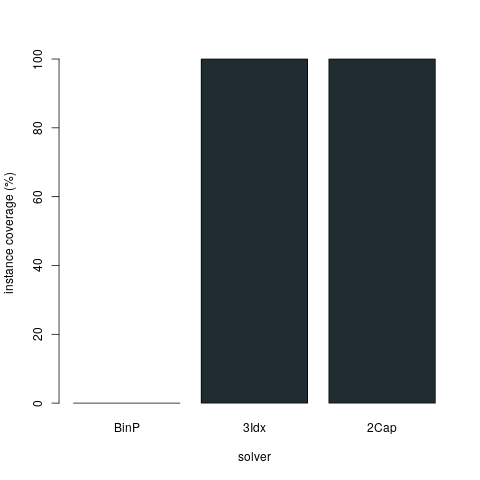
\includegraphics[width=1.2\textwidth]{img/solver_instance_coverage_b=2_s_1s.png}
\caption{\textsc{Zeitlimit 1s}}
\label{fig:instance_cov_b=2_s_a}
\end{subfigure}
\hfill
\begin{subfigure}[b]{0.3\textwidth}
\centering
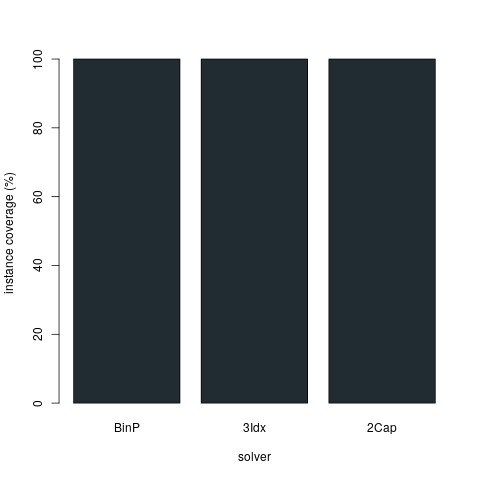
\includegraphics[width=1.2\textwidth]{img/solver_instance_coverage_b=2_s_3s.png}
\caption{\textsc{Zeitlimit 3s}}
\label{fig:instance_cov_b=2_s_b}
\end{subfigure}
\hfill
\begin{subfigure}[b]{0.3\textwidth}
\centering
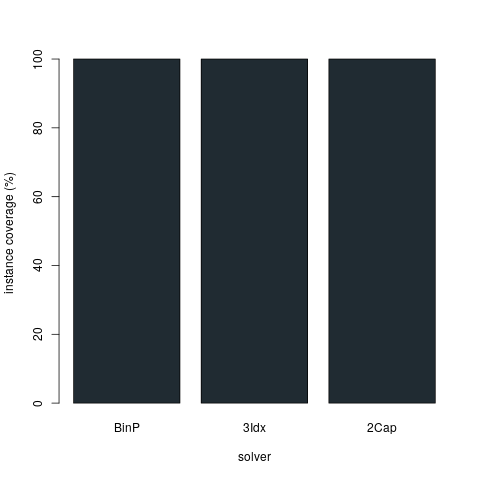
\includegraphics[width=1.2\textwidth]{img/solver_instance_coverage_b=2_s_5s.png}
\caption{\textsc{Zeitlimit 5s}}
\label{fig:instance_cov_b=2_s_c}
\end{subfigure}

\caption{\textsc{Instance-Coverage der $b=2$ Solver (s)}}
\label{fig:instance_cov_b=2_s}
\end{figure}

\pagebreak

In Abb. \ref{fig:b=2_s_runtimes} sind die Laufzeiten der Solver pro Instanz in Sekunden bei einem Zeitlimit von $5s$ dargestellt.
Man erkennt, dass die 3-Index-Formulierung deutlich schneller ist als die Bin-Packing-Formulierung und, dass die Heuristik beide MIP-Formulierungen noch einmal deutlich unterbietet. Da in der Abb. nur die absoluten Laufzeitdifferenzen zu sehen sind,
ist es wichtig, zu erwähnen, dass die Laufzeiten der Heuristik durchschnittlich um den Faktor $55.0$ kleiner sind,
als die der 3-Index-Formulierung. Zwischen der 3-Index- und der Bin-Packing-Formulierung liegt dagegen nur ein Faktor von $2.7$.

Aufgrund der Tatsache, dass CPLEX nur dann vor dem Zeitlimit terminiert, wenn die Instanz optimal gelöst wurde, ist klar
ersichtlich, dass die 3-Index-Formulierung sämtliche Instanzen nach etwa $1s$ optimal löst während die Bin-Packing-Formulierung in wenigen Fällen durch das Zeitlimit gestoppt wird.\newline
Bei den Instanzen $01$ und $08$, bei denen die Bin-Packing-Formulierung durch das Zeitlimit gestoppt wurde und dementsprechend nicht
notwendigerweise eine optimale Lösung gefunden hat, konnte die Heuristik, wie man Abb. \ref{fig:b=2_s_costs} entnehmen kann, sogar
bessere Zielfunktionswerte erzielen als die Bin-Packing-Formulierung.\newline
Die weiteren Zielfunktionswerte der Bin-Packing-Formulierung sind in Abb. \ref{fig:b=2_s_costs}  deshalb nicht zu erkennen,
weil sie durch die Zielfunktionswerte der 3-Index-Formulierung verdeckt werden. Da beide Formulierungen die entsprechenden
Instanzen optimal lösen, kommen sie jeweils zum selben Zielfunktionswert.

\begin{figure}[H]
\centering
\begin{subfigure}[b]{0.4\textwidth}
\centering
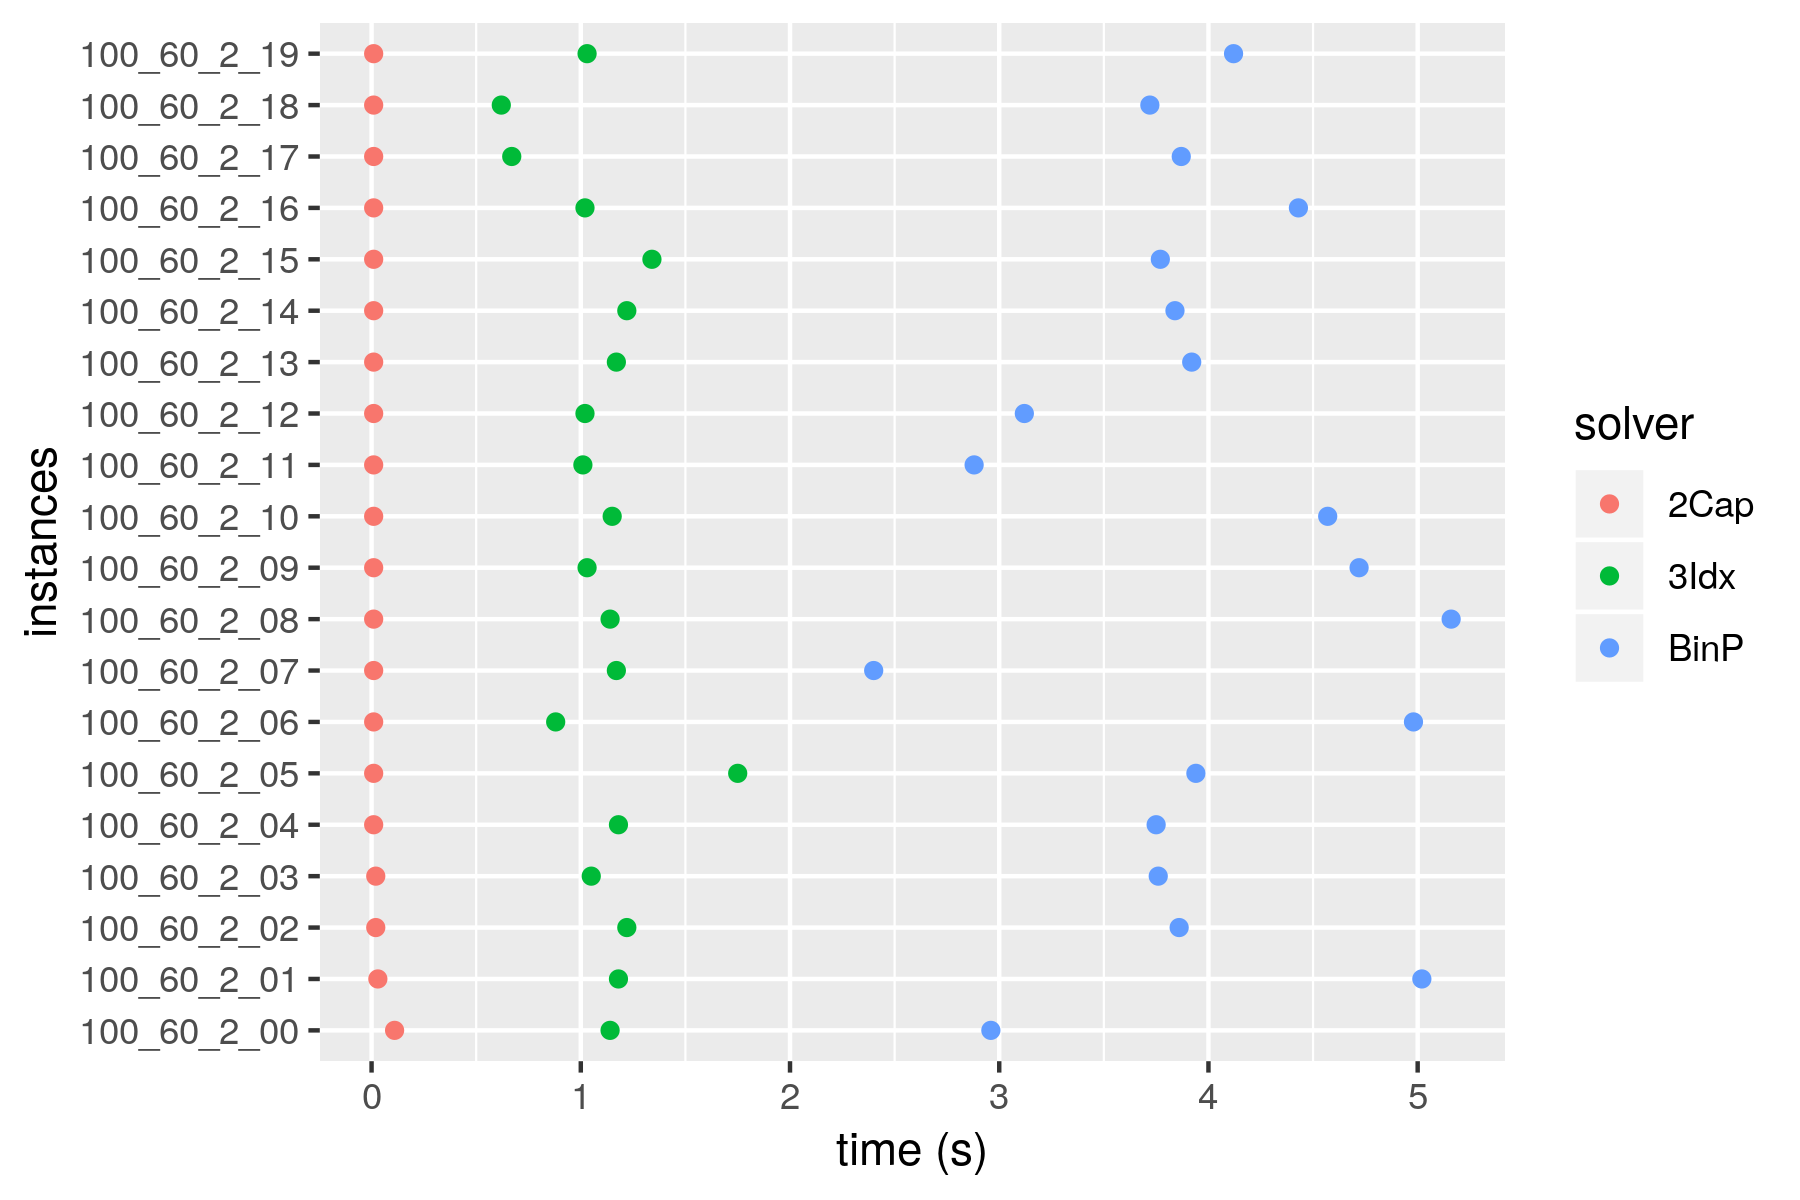
\includegraphics[width=1.3\textwidth]{img/solver_instance_time_b=2_s_5s.png}
\caption{\textsc{Laufzeiten bei 5s Zeitlimit}}
\label{fig:b=2_s_runtimes}
\end{subfigure}
\hfill
\begin{subfigure}[b]{0.4\textwidth}
\centering
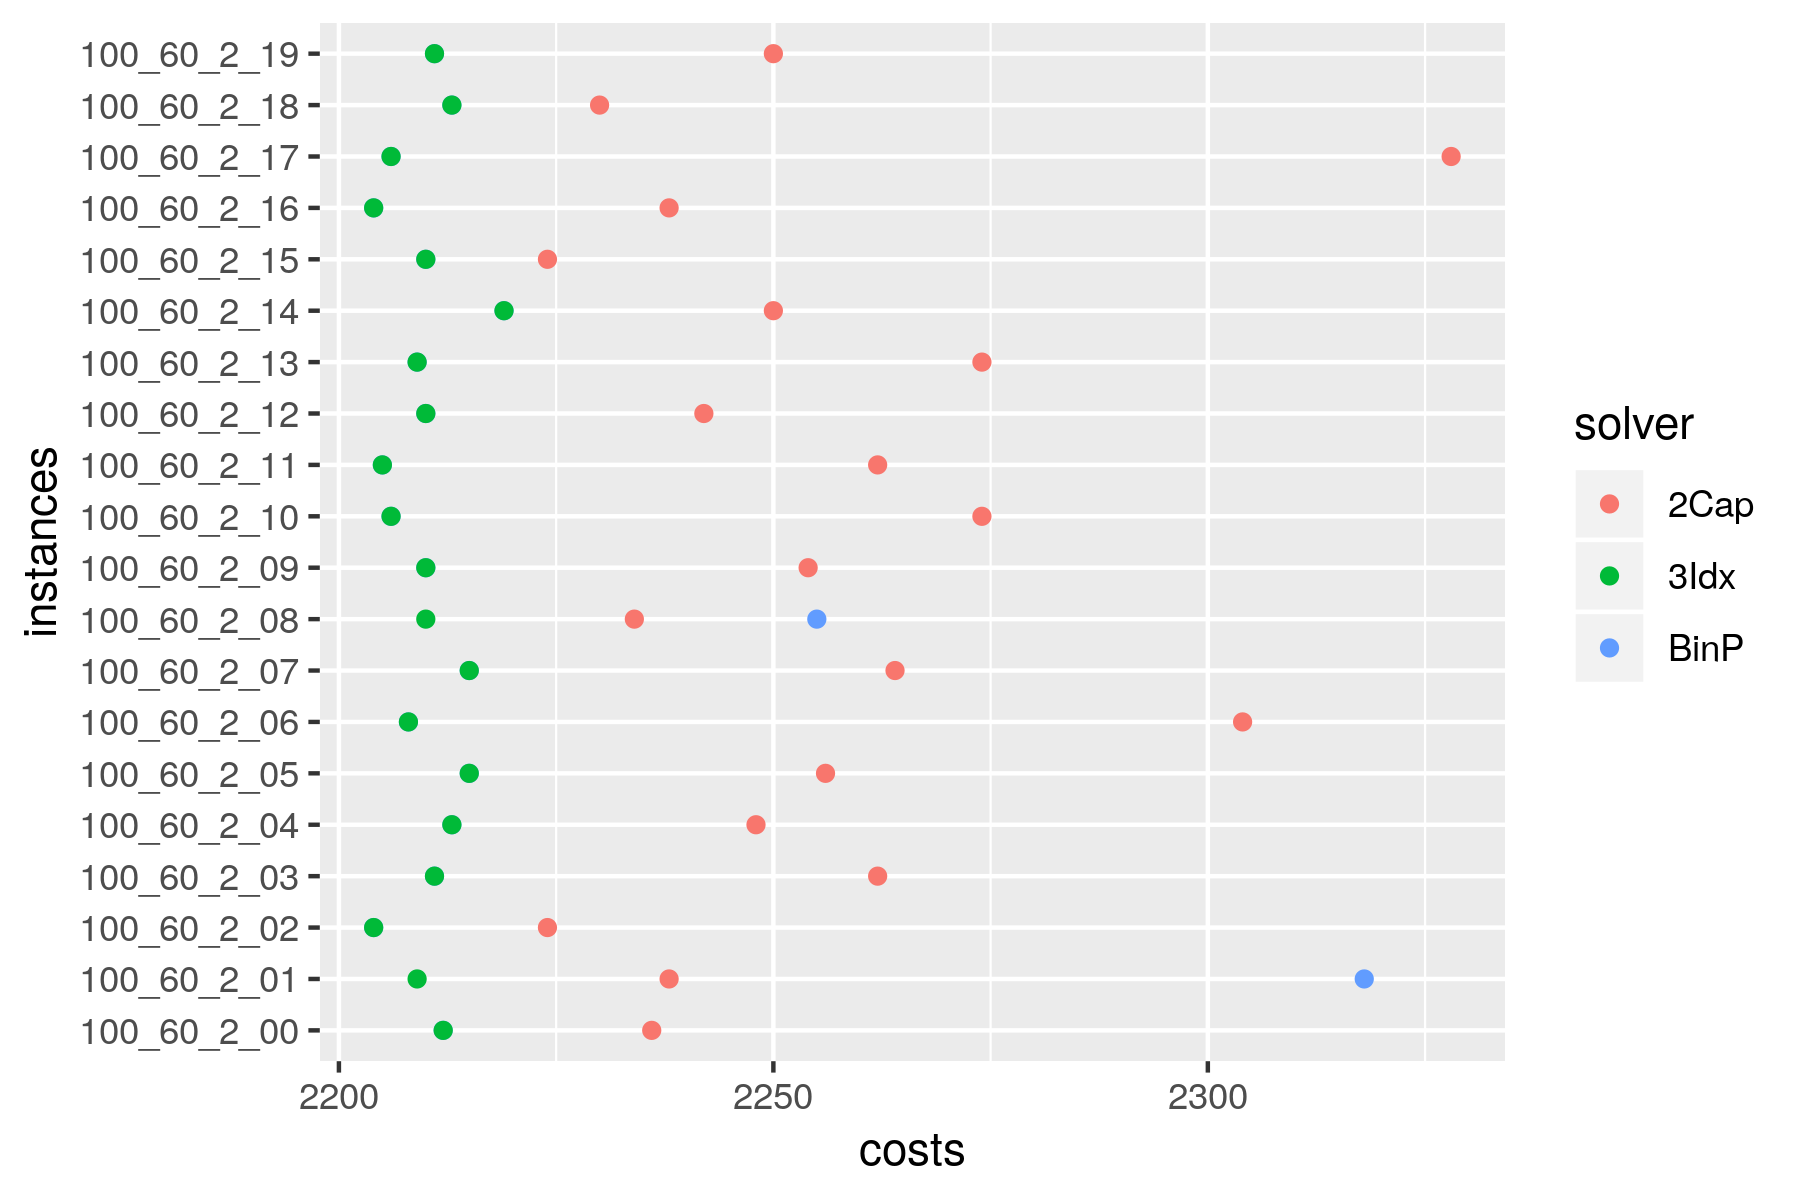
\includegraphics[width=1.3\textwidth]{img/solver_instance_cost_b=2_s_5s.png}
\caption{\textsc{Kosten bei 5s Zeitlimit}}
\label{fig:b=2_s_costs}
\end{subfigure}
\caption{}
\end{figure}

Die exakten Ergebnisse der MIP-Formulierungen sind den Tabellen in Abb. \ref{fig:table} zu entnehmen.
\textquote{Optimal} bezeichnet den prozentualen Anteil der Instanzen, die optimal gelöst wurden. Bei der Laufzeit handelt
es sich um die durchschnittliche Laufzeit pro Instanz in Sekunden und die Abweichung gibt die durchschnittliche prozentuale Abweichung
vom optimalen Zielfunktionswert pro Instanz an.

\begin{figure}[H]
\centering

\begin{subfigure}[b]{0.3\textwidth}
\centering
\resizebox{\textwidth}{!}{
\begin{tabular}{ | l | l | l |}
    \hline
     & \textbf{BinP} & \textbf{3Idx} \\ \hline
    \textbf{Optimal} & $ \textcolor{red}{0 \%}$ & $ \textcolor{mygreen}{35 \%}$ \\ \hline
    \textbf{Laufzeit} & $\textcolor{red}{---}$ & \O $\thinspace \textcolor{mygreen}{0.9 s}$ \\ \hline
    \textbf{Abweichung} & $\textcolor{red}{---}$ & \O $\thinspace \textcolor{mygreen}{2.0 \%}$ \\ \hline
\end{tabular}}
\caption{\textsc{Zeitlimit} $1s$}
\label{fig:res_b=2_s_a}
\end{subfigure}
% $\quad\quad\quad\quad$
\begin{subfigure}[b]{0.3\textwidth}
\centering
\resizebox{\textwidth}{!}{
\begin{tabular}{ | l | l | l |}
    \hline
     & \textbf{BinP} & \textbf{3Idx} \\ \hline
    \textbf{Optimal} & $ \textcolor{red}{10 \%}$ & $ \textcolor{mygreen}{100 \%}$ \\ \hline
    \textbf{Laufzeit} & \O $\thinspace \textcolor{red}{3.0 s}$ & \O $\thinspace \textcolor{mygreen}{1.1 s}$ \\ \hline
    \textbf{Abweichung} & \O $\thinspace \textcolor{red}{4.7 \%}$ & \O $\thinspace \textcolor{mygreen}{0.0 \%}$ \\ \hline
\end{tabular}}
\caption{\textsc{Zeitlimit} $3s$}
\label{fig:res_b=2_s_b}
\end{subfigure}
% \end{figure}
% \begin{figure}[H]
\begin{subfigure}[b]{0.3\textwidth}
\centering
\resizebox{\textwidth}{!}{
\begin{tabular}{ | l | l | l |}
    \hline
     & \textbf{BinP} & \textbf{3Idx} \\ \hline
    \textbf{Optimal} & $ \textcolor{red}{90 \%}$ & $ \textcolor{mygreen}{100 \%}$ \\ \hline
    \textbf{Laufzeit} & \O $\thinspace \textcolor{red}{3.9 s}$ & \O $\thinspace \textcolor{mygreen}{1.1 s}$ \\ \hline
    \textbf{Abweichung} & \O $\thinspace \textcolor{red}{0.4 \%}$ & \O $\thinspace \textcolor{mygreen}{0.0 \%}$ \\ \hline
\end{tabular}}
\caption{\textsc{Zeitlimit} $5s$}
\label{fig:res_b=2_s_c}
\end{subfigure}

\caption{\textsc{MIP-Ergebnisse}}
\label{fig:table}
\end{figure}

Abbildung \ref{fig:table} zeigt, dass die 3-Index-Formulierung bei jedem betrachteten Zeitlimit eine geringere Laufzeit benötigt
als die Bin-Packing-Formulierung und somit zu besseren Ergebnissen kommt.

Da die Zeitlimits aufgrund der geringen Laufzeit für die Heuristik keine Rolle spielen, kommt diese stets zum selben Ergebnis.
Sie weicht durchschnittlich um $2.0 \%$ vom Optimum ab und benötigt dafür eine Laufzeit von nur $0.02s$.

Trotz dieser guten Ergebnisse der Heuristik, besteht aufgrund der Tatsache, dass die 3-Index-Formulierung sämtliche Instanzen
mit einer durchschnittlichen Laufzeit von $1.1s$ optimal löst, aus praktischer Perspektive vermutlich kein großer Bedarf für
eine Laufzeitverbesserung durch eine Heuristik.

\textbf{Mittelgroße Instanzen (m)}

Interessanter wird es bereits beim Vergleich der Solver für in Kapitel \ref{sec:test_data} als mittelgroß bezeichnete Instanzen,
bei denen es darum geht, $300$ eintreffende Items in die Storage-Area zu verladen.
In Abb. \ref{fig:instance_cov_b=2} ist erneut die Instance-Coverage der einzelnen Solver dargestelllt.

In Abb. \ref{fig:instance_cov_b=2_m_a} sieht man, dass die Bin-Packing-Formulierung nach einer Minute noch keine Instanz gelöst hat, während die
3-Index-Formulierung dort bereits $80 \%$ der Instanzen löst. Selbst bei einem Zeitlimit von $10$ Minuten pro Instanz löst die Bin-Packing-Formulierung nur $20 \%$ der Instanzen, 3-Index löst bei diesem Zeitlimit sämtliche Instanzen
(vgl. Abb. \ref{fig:instance_cov_b=2_m_b}).
Bei einem Zeitlimit von $20$ Minuten löst schließlich auch die Bin-Packing-Formulierung sämtliche Instanzen
(vgl. Abb. \ref{fig:instance_cov_b=2_m_c}). Die Heuristik löst, wie bereits in der Kategorie der kleinen Instanzen,
in jedem Fall sämtliche Instanzen.
\begin{figure}[H]
\centering

\begin{subfigure}[b]{0.3\textwidth}
\centering
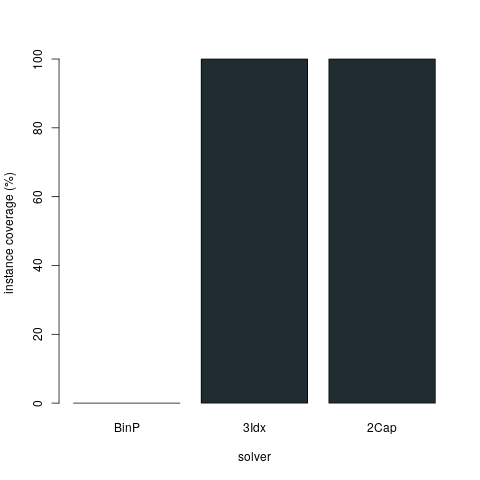
\includegraphics[width=1.2\textwidth]{img/solver_instance_coverage_b=2_m_60s.png}
\caption{\textsc{Zeitlimit} $1min$}
\label{fig:instance_cov_b=2_m_a}
\end{subfigure}
\hfill
\begin{subfigure}[b]{0.3\textwidth}
\centering
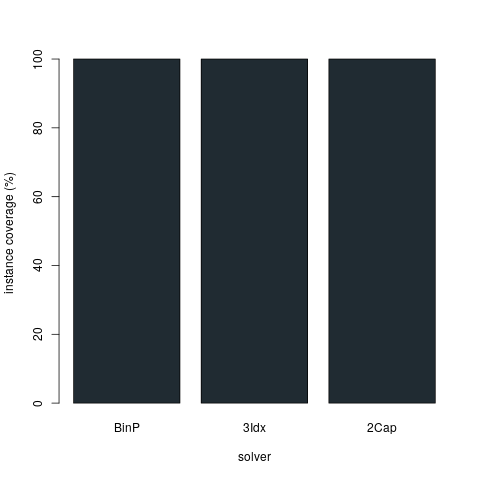
\includegraphics[width=1.2\textwidth]{img/solver_instance_coverage_b=2_m_600s.png}
\caption{\textsc{Zeitlimit} $10min$}
\label{fig:instance_cov_b=2_m_b}
\end{subfigure}
\hfill
\begin{subfigure}[b]{0.3\textwidth}
\centering
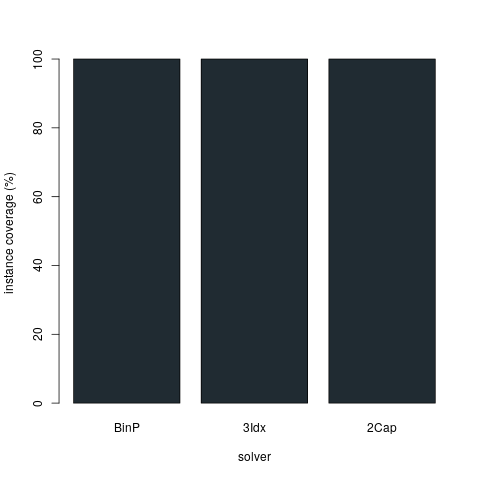
\includegraphics[width=1.2\textwidth]{img/solver_instance_coverage_b=2_m_1200s.png}
\caption{\textsc{Zeitlimit} $20min$}
\label{fig:instance_cov_b=2_m_c}
\end{subfigure}
\caption{\textsc{Instance-Coverage der $b=2$ Solver (m)}}
\label{fig:instance_cov_b=2}
\end{figure}

Da die Zeitlimits aufgrund der geringen Laufzeit der Heuristik für diese erneut keine Rolle spielen,
kommt sie stets zum selben Ergebnis. Sie weicht durchschnittlich um $0.8 \%$ vom
Optimum ab und benötigt dafür eine Laufzeit von $0.1s$.

\pagebreak

In Abb. \ref{fig:res_plots_b=2_m} sind die Laufzeiten und ermittelten Zielfunktionswerte der Solver bei einem Zeitlimit von $20$
Minuten dargestellt. Da die Bin-Packing- und die 3-Index-Formulierung bei diesem Zeitlimit sämtliche Instanzen optimal lösen,
kommen sie stets zum selben Kostenwert (vgl. Abb \ref{fig:b=2_m_costs}),
wobei die Bin-Packing-Einträge in der Visualisierung erneut durch die Einträge der 3-Index-Formulierung verdeckt werden.
In Abb. \ref{fig:b=2_m_runtimes} ist gut zu erkennen, dass die Bin-Packing-Formulierung deutlich längere Laufzeiten als die 3-Index-Formulierung
und die Heurisktik benötigt, wobei die Heuristik noch einmal deutlich schneller ist. Dabei handelt es sich allerdings um die absoluten Laufeiten.
Im Wesentlichen ist der Laufzeitunterschied zwischen der Heuristik und der 3-Index-Formulierung deutlich größer, als jener zwischen den beiden
MIP-Formulierungen. Zwischen der Heuristik, welche durchschnittlich $0.1s$ benötigt und der 3-Index-Formulierung, die durchschnittlich $107.8s$ benötigt (vgl. Abb. \ref{fig:res_b=2_m_c}), besteht ein Faktor von $1077.0$ während zwischen den beiden MIP-Formulierungen nur ein Faktor von
$7.1$ besteht. Die absolute Darstellung ist in diesem Fall also etwas irreführend, da die Heuristik deutlich schneller ist als beide MIP-Formulierungen. Trotzdem würde man in diesem Fall aus praktischer Perspektive die 3-Index-Formulierung klar der Bin-Packing-Formulierung vorziehen, dieser Sachverhalt ist in Abb. \ref{fig:b=2_m_runtimes} gut erkennbar.

\begin{figure}[H]
\centering
\begin{subfigure}[b]{0.4\textwidth}
\centering
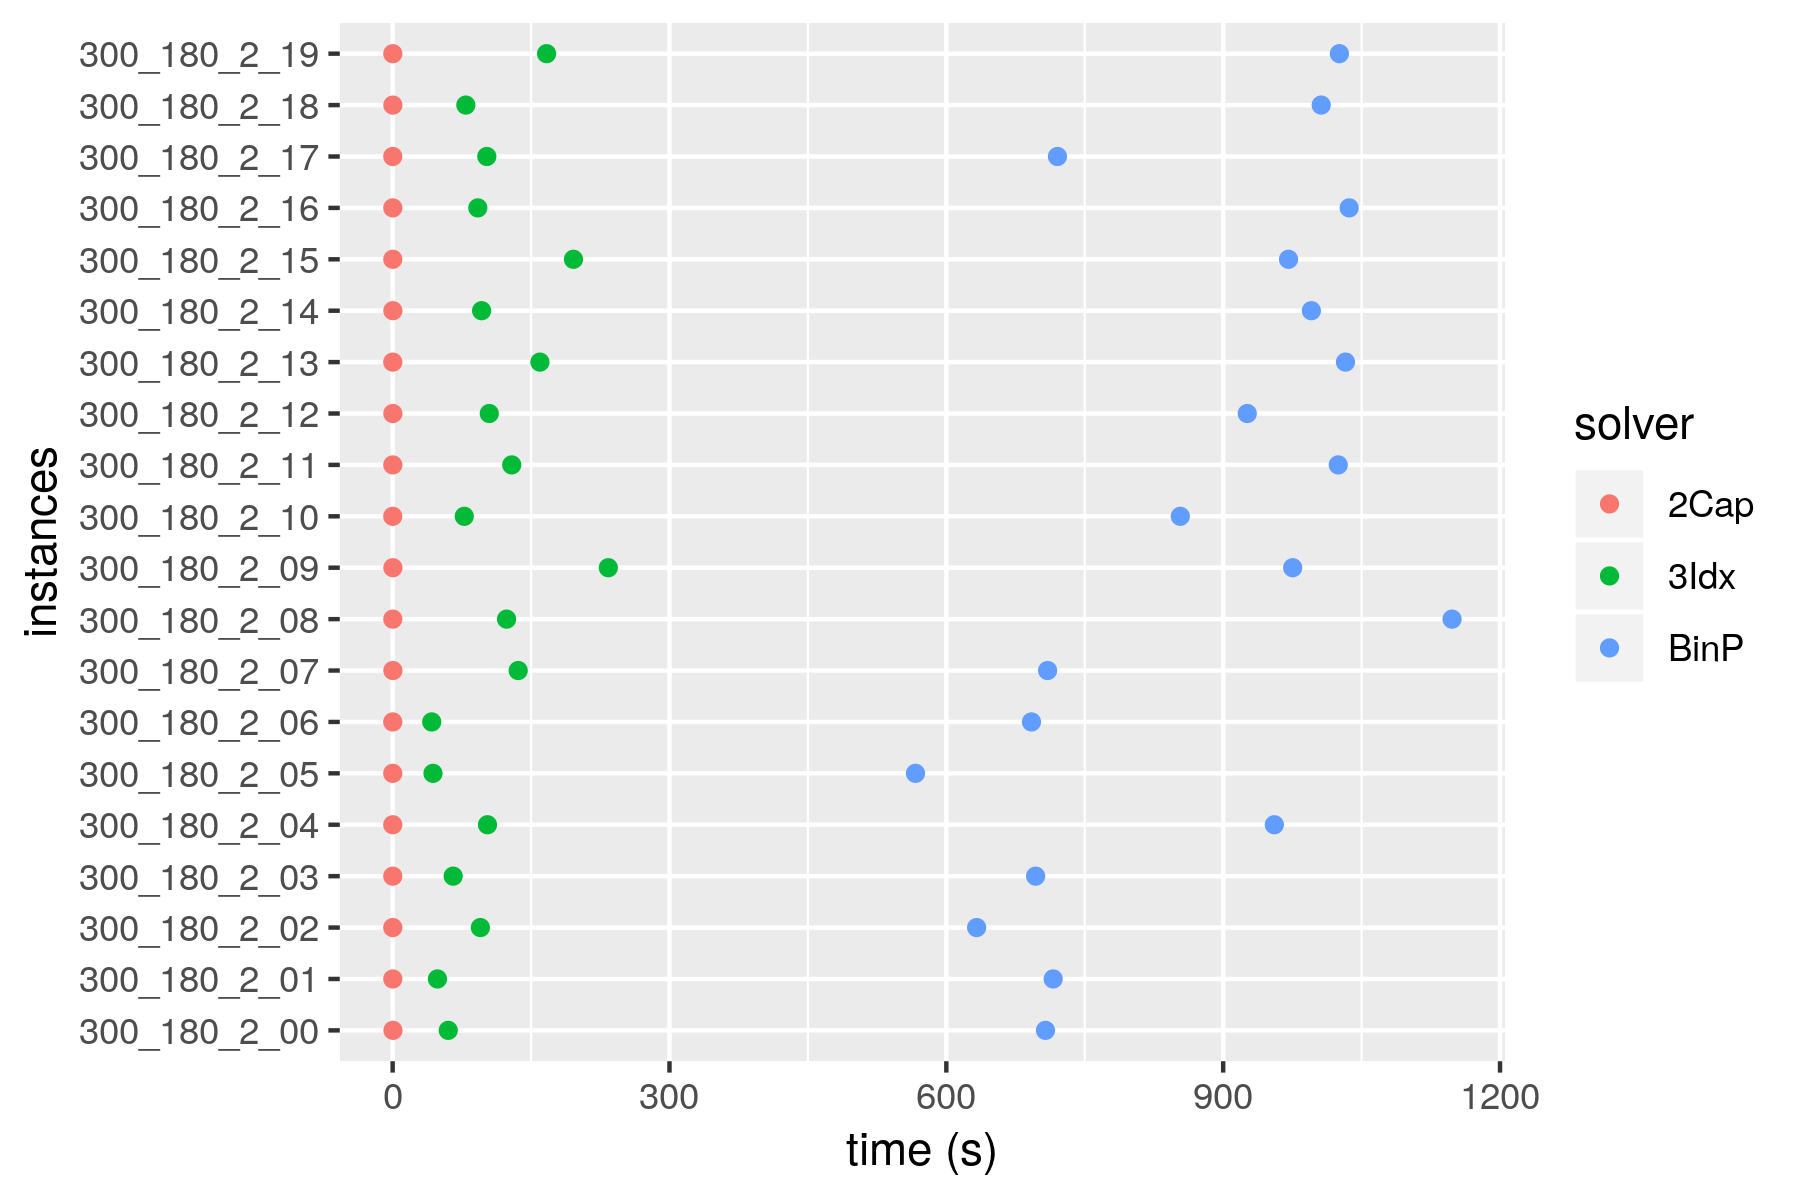
\includegraphics[width=1.3\textwidth]{img/solver_instance_time_b=2_m_1200s.png}
\caption{\textsc{Laufzeiten bei $20min$ Limit}}
\label{fig:b=2_m_runtimes}
\end{subfigure}
\hfill
\begin{subfigure}[b]{0.4\textwidth}
\centering
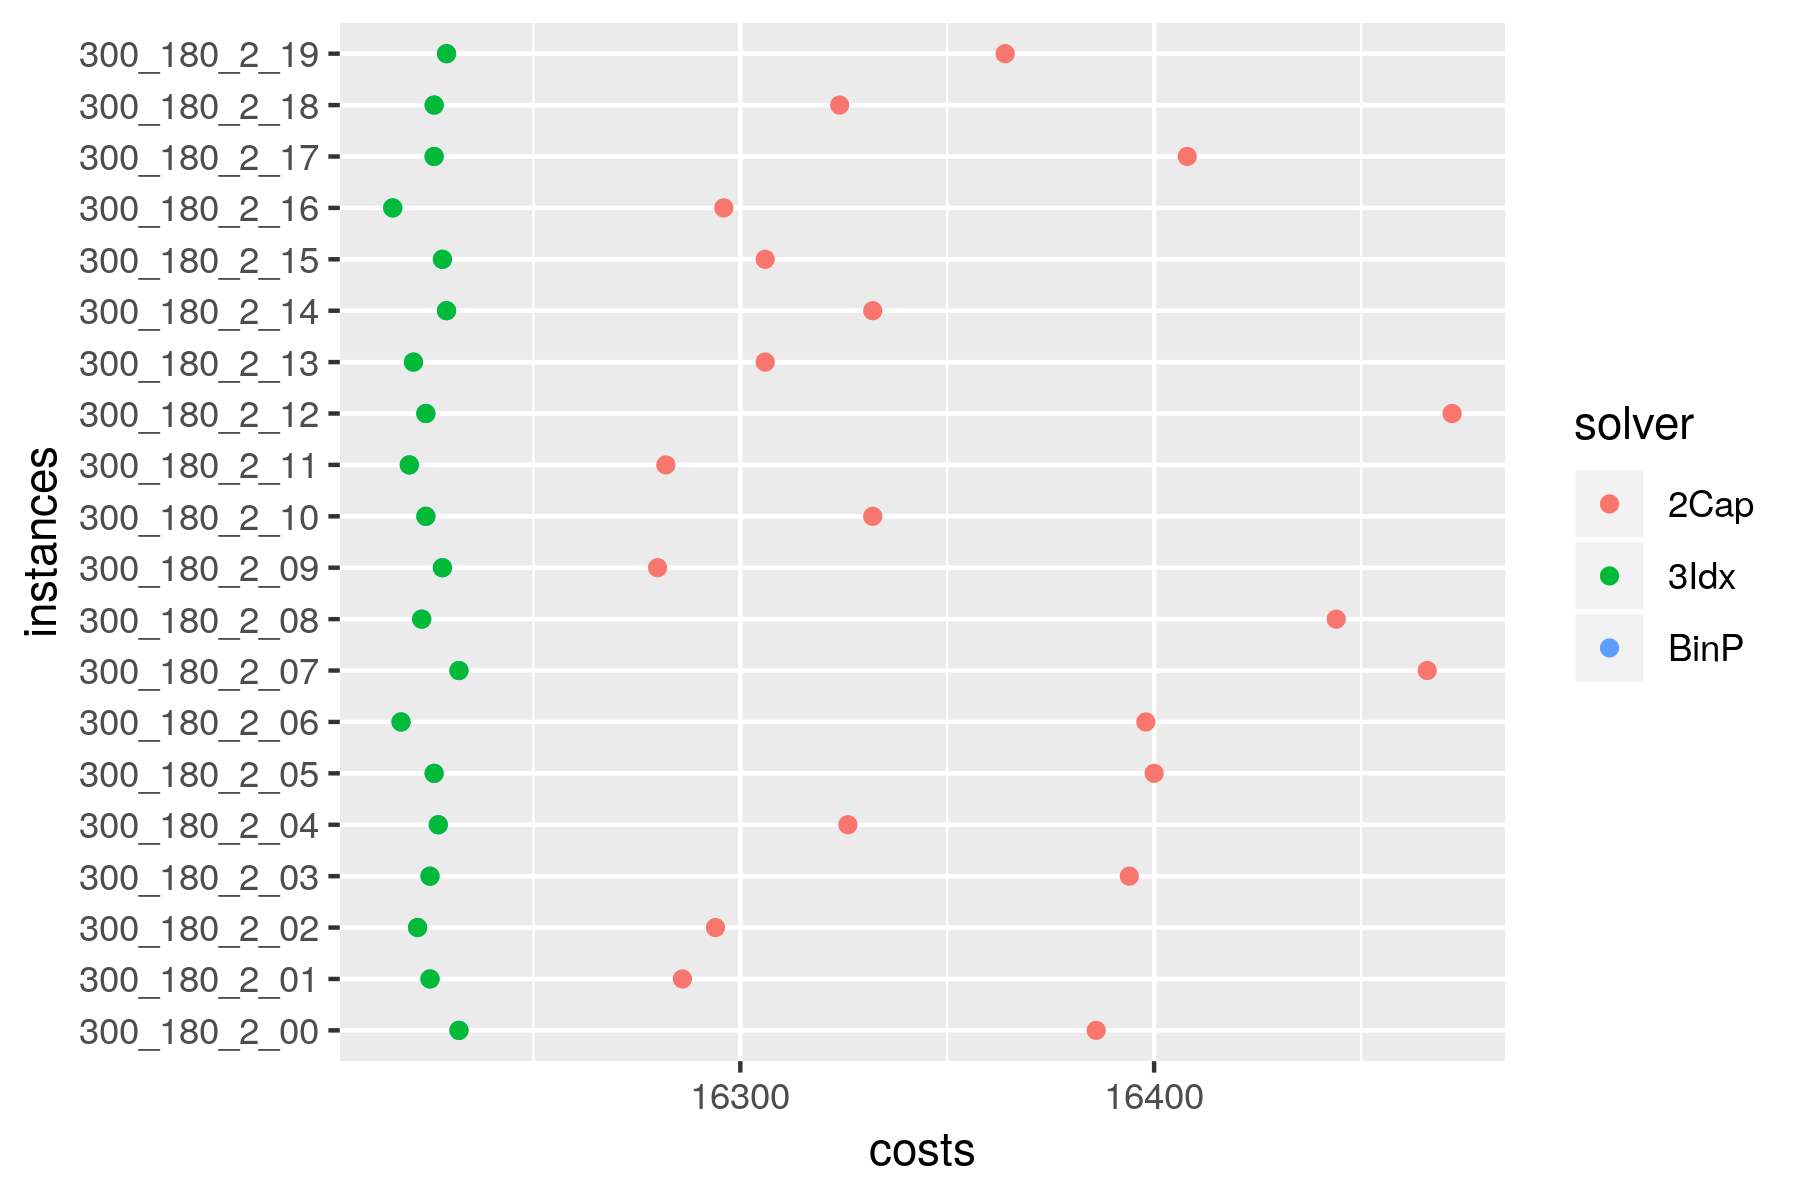
\includegraphics[width=1.3\textwidth]{img/solver_instance_cost_b=2_m_1200s.png}
\caption{\textsc{Kosten bei $20min$ Limit}}
\label{fig:b=2_m_costs}
\end{subfigure}
\caption{}
\label{fig:res_plots_b=2_m}
\end{figure}

In den Tabellen in Abb. \ref{fig:res_b=2_m} können die exakten Ergebnisse der MIP-Formulierungen nachvollzogen werden.
Wie bereits erwähnt, hat die Bin-Packing-Formulierung bei einem Zeitlimit von einer Minute keine Instanz gelöst, die 3-Index-Formulierung löst
$80 \%$ der Instanzen, allerdings nur $50 \%$ optimal (vgl. \ref{fig:res_b=2_m_a}). Die 3-Index-Formulierung benötigt dafür durchschnittlich
$55.4s$ und weicht, genau wie die Heuristik, um durchschnittlich $0.8 \%$ vom Optimum ab. Die Heuristik löst dabei allerdings sämtliche Instanzen
und benötigt nur durchschnittlich $0.1s$.

\begin{figure}[H]
% \end{figure}
% \begin{figure}[H]
% $\quad\quad\quad\quad$
\begin{subfigure}[b]{0.3\textwidth}
\centering
\resizebox{\textwidth}{!}{
\begin{tabular}{ | l | l | l |}
    \hline
     & \textbf{BinP} & \textbf{3Idx} \\ \hline
    \textbf{Optimal} & $ \textcolor{red}{0 \%}$ & $ \textcolor{mygreen}{50 \%}$ \\ \hline
    \textbf{Laufzeit} & $\textcolor{red}{----}$ & \O $\thinspace \textcolor{mygreen}{55.4 s}$ \\ \hline
    \textbf{Abweichung} & $\textcolor{red}{----}$ & \O $\thinspace \textcolor{mygreen}{0.8 \%}$ \\ \hline
\end{tabular}}
\caption{\textsc{Zeitlimit} $1min$}
\label{fig:res_b=2_m_a}
\end{subfigure}
\begin{subfigure}[b]{0.3\textwidth}
\centering
\resizebox{\textwidth}{!}{
\begin{tabular}{ | l | l | l |}
    \hline
     & \textbf{BinP} & \textbf{3Idx} \\ \hline
    \textbf{Optimal} & $ \textcolor{red}{10 \%}$ & $ \textcolor{mygreen}{100 \%}$ \\ \hline
    \textbf{Laufzeit} & \O $\thinspace \textcolor{red}{581.6 s}$ & \O $\thinspace \textcolor{mygreen}{73.7 s}$ \\ \hline
    \textbf{Abweichung} & \O $\thinspace \textcolor{red}{0.6 \%}$ & \O $\thinspace \textcolor{mygreen}{0.0 \%}$ \\ \hline
\end{tabular}}
\caption{\textsc{Zeitlimit} $10min$}
\label{fig:res_b=2_m_b}
\end{subfigure}
% \end{figure}
% \begin{figure}[H]
\begin{subfigure}[b]{0.3\textwidth}
\centering
\resizebox{\textwidth}{!}{
\begin{tabular}{ | l | l | l |}
    \hline
     & \textbf{BinP} & \textbf{3Idx} \\ \hline
    \textbf{Optimal} & $ 100 \%$ & $ 100 \%$ \\ \hline
    \textbf{Laufzeit} & \O $\thinspace 869.6 s$ & \O $\thinspace \textcolor{mygreen}{107.8 s}$ \\ \hline
    \textbf{Abweichung} & \O $\thinspace 0.0 \%$ & \O $\thinspace 0.0 \%$ \\ \hline
\end{tabular}}
\caption{\textsc{Zeitlimit} $20min$}
\label{fig:res_b=2_m_c}
\end{subfigure}
\caption{\textsc{MIP-Ergebnisse}}
\label{fig:res_b=2_m}
\end{figure}

Zusammenfassend ist die 3-Index-Formulierung in der Kategorie der mittelgroßen Instanzen der Bin-Packing-Formulierung vorzuziehen,
da sie bei allen betrachteten Zeitlimits die besseren Ergebnisse erzielt und auch bei einem Zeitlimit von $20$ Minuten, bei dem schließlich auch die Bin-Packing-Formulierung sämtliche Instanzen optimal löst, deutlich schneller ist als diese.

Die zu bevorzugende MIP-Formulierung 3-Index, benötigt, wie sich Abb. \ref{fig:res_b=2_m_b} entnehmen lässt, durchschnittlich
$73.7s$ um sämtliche Instanzen optimal zu lösen. Die Heuristik dagegen benötigt durchschnittlich $0.1s$ um sämtliche Instanzen
mit einer durchschnittlichen Abweichung vom Optimum von $0.8 \%$ zu lösen.

Dieser Laufzeitunterschied ist so erheblich, dass die gerine Abweichung vom Optimum in der Praxis vermutlich in Kauf genommen werden kann,
wenn sich dadurch eine derart große Laufzeitersparnis ergibt. In dieser Kategorie stellt sich die Heuristik demzufolge als sehr gute Alternative
heraus.

\textbf{Große Instanzen (l)}

Zuletzt werden die Solver für die in Kapitel \ref{sec:test_data} als groß bezeichneten Instanzen, bei denen es darum geht,
$500$ eintreffende Items in die Storage-Area zu verladen, verglichen. In dieser Kategorie wurden noch einmal größere Zeitlimits von
$15$, $30$ und $45$ Minuten betrachtet.

In Abb. \ref{fig:instance_cov_b=2_l} ist die Instance-Coverage der Solver für die jeweiligen Zeitlimits dargestellt und es fällt auf,
dass die Bin-Packing-Formulierung erst bei einem Zeitlimit von $45$ Minuten überhaupt eine Instanz löst (vgl. \ref{fig:instance_cov_b=2_l_c}).
In diesem Szenario ist die 3-Index-Formulierung der Bin-Packing-Formulierung folglich klar überlegen.

\begin{figure}[H]
\centering

\begin{subfigure}[b]{0.3\textwidth}
\centering
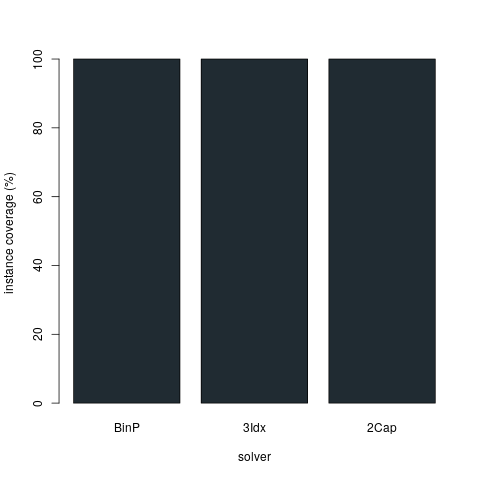
\includegraphics[width=1.2\textwidth]{img/solver_instance_coverage_b=2_l_900s.png}
\caption{\textsc{Zeitlimit} $15min$}
\label{fig:instance_cov_b=2_l_a}
\end{subfigure}
\hfill
\begin{subfigure}[b]{0.3\textwidth}
\centering
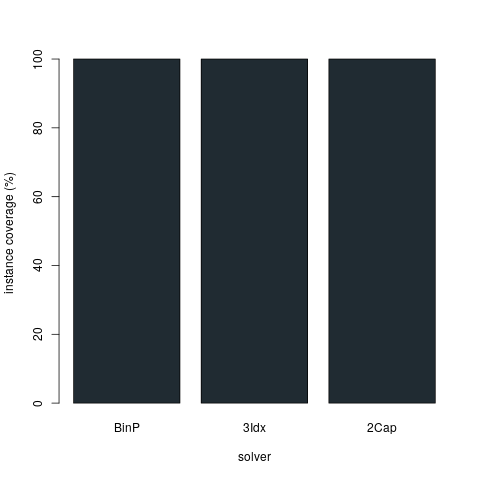
\includegraphics[width=1.2\textwidth]{img/solver_instance_coverage_b=2_l_1800s.png}
\caption{\textsc{Zeitlimit} $30min$}
\label{fig:instance_cov_b=2_l_b}
\end{subfigure}
\hfill
\begin{subfigure}[b]{0.3\textwidth}
\centering
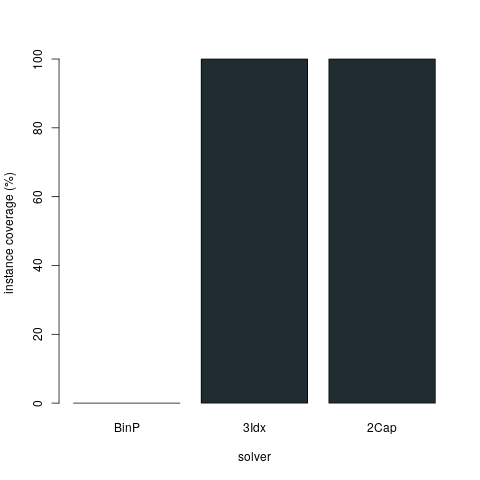
\includegraphics[width=1.2\textwidth]{img/solver_instance_coverage_b=2_l_2700s.png}
\caption{\textsc{Zeitlimit} $45min$}
\label{fig:instance_cov_b=2_l_c}
\end{subfigure}

\caption{\textsc{Instance-Coverage der $b=2$ Solver (l)}}
\label{fig:instance_cov_b=2_l}
\end{figure}

Überdies ist Abb. \ref{fig:instance_cov_b=2_l} zu enthnehmen, dass die 3-Index-Formulierung erst beim betrachteten
Zeitlimit von $45$ Minuten sämtliche Instanzen gelöst hat. Für die Heuristik sind die Zeitlimits erneut irrelevant,
da sie mit einer durchschnittlichen Laufzeit von $0.7s$ pro Instanz sämtliche Instanzen löst.

\pagebreak

In Abb. \ref{fig:res_plots_b=2_l} bestätigt sich die Tendenz aus der Darstellung der Instance-Coverage.
Die Heuristik ist deutlich schneller als die 3-Index-Formulierung (vgl. Abb \ref{fig:b=2_l_runtimes}) und weicht dabei nur
unwesentlich vom optimalen Zielfunktionswert ab (vgl. \ref{fig:b=2_l_costs}). Wie bereits zuvor gesehen, löst
die Bin-Packing-Formulierung mit Instanz $09$ nur eine einzige Instanz und reizt dafür, wie man Abb. \ref{fig:b=2_l_runtimes}
entnehmen kann, das Zeitlimit von $45$ Minuten vollständig aus. In Abb. \ref{fig:b=2_l_costs} ist zu erkennen, dass diese auch bei den
Zielfunktionswerten sehr weit von denen der 3-Index-Formulierung und der Heuristik abweicht und somit in dieser Kategorie in keinem Fall
konkurrenzfähig ist.

\begin{figure}[H]
\centering
\begin{subfigure}[b]{0.4\textwidth}
\centering
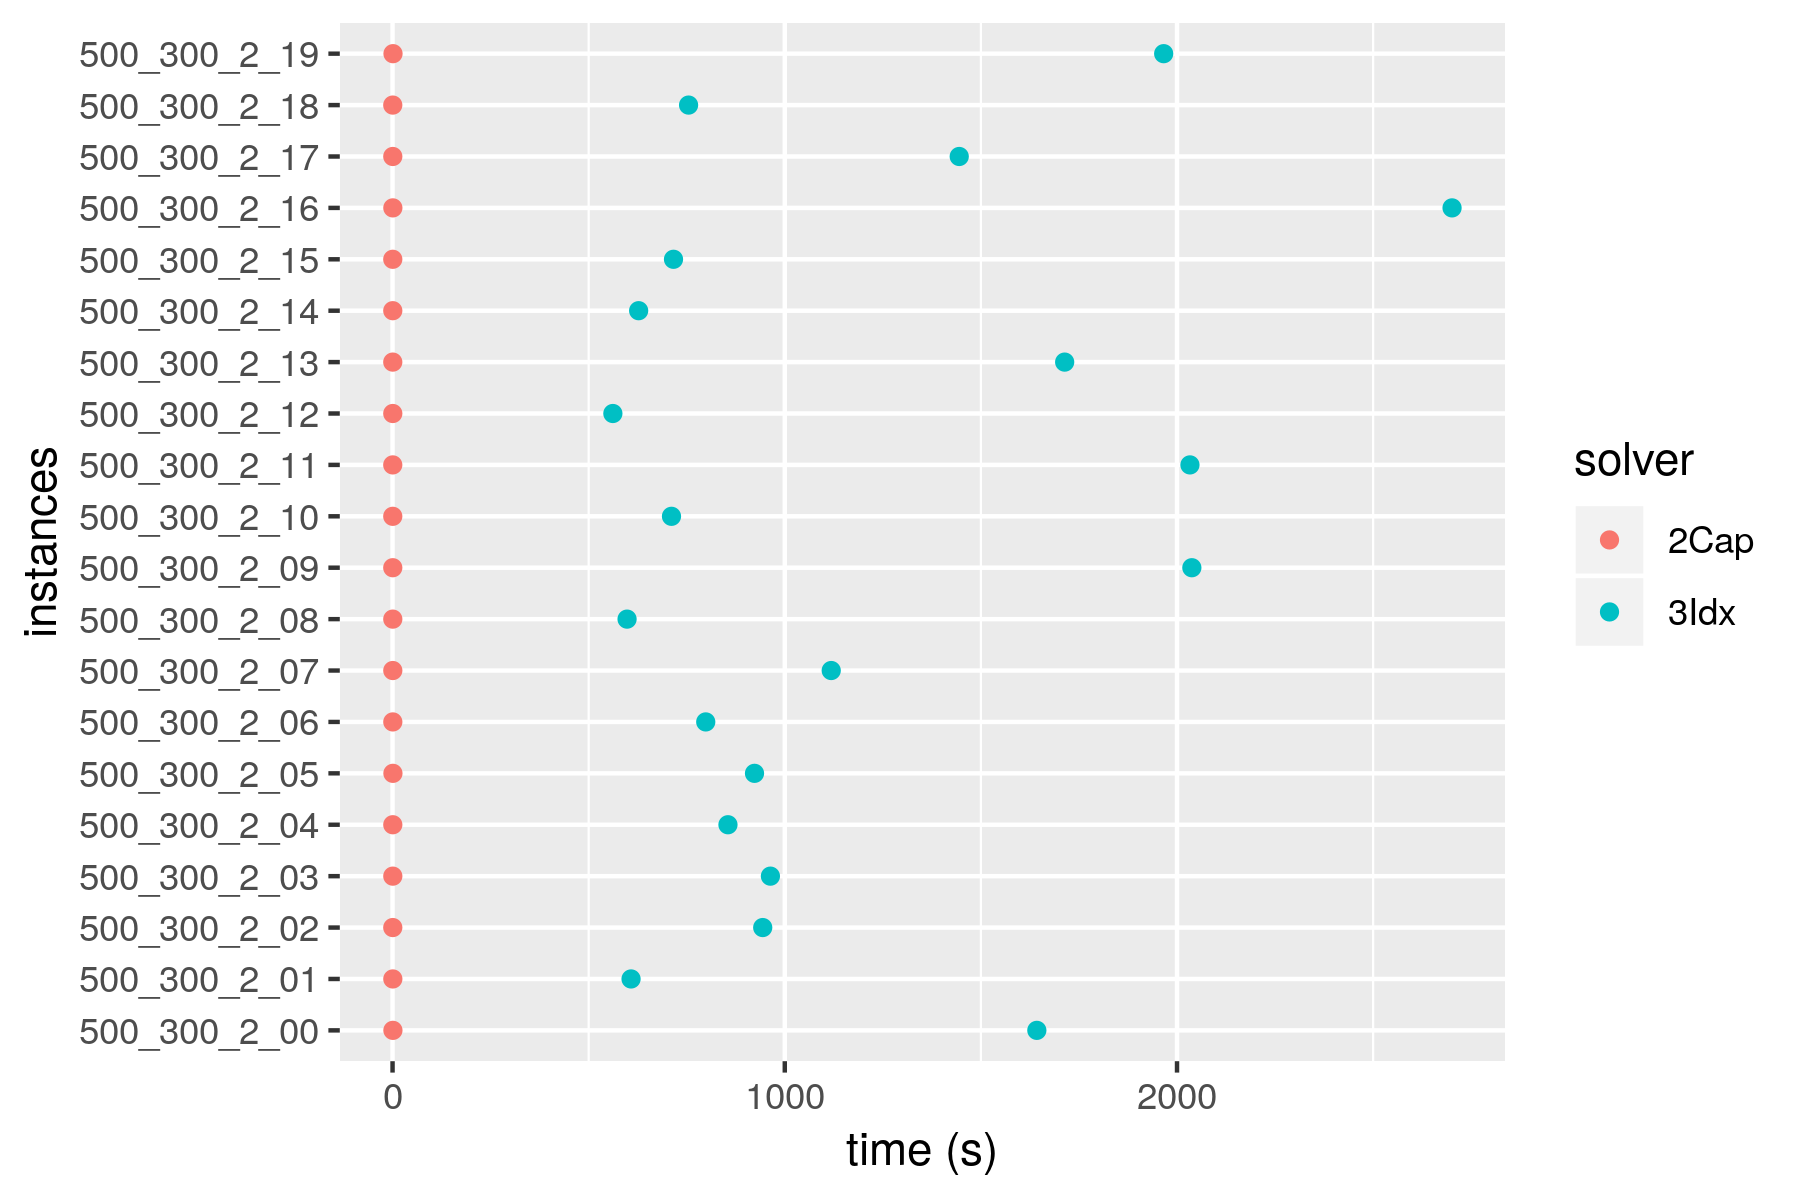
\includegraphics[width=1.3\textwidth]{img/solver_instance_time_b=2_l_2700s.png}
\caption{\textsc{Laufzeiten bei $45min$ Limit}}
\label{fig:b=2_l_runtimes}
\end{subfigure}
\hfill
\begin{subfigure}[b]{0.4\textwidth}
\centering
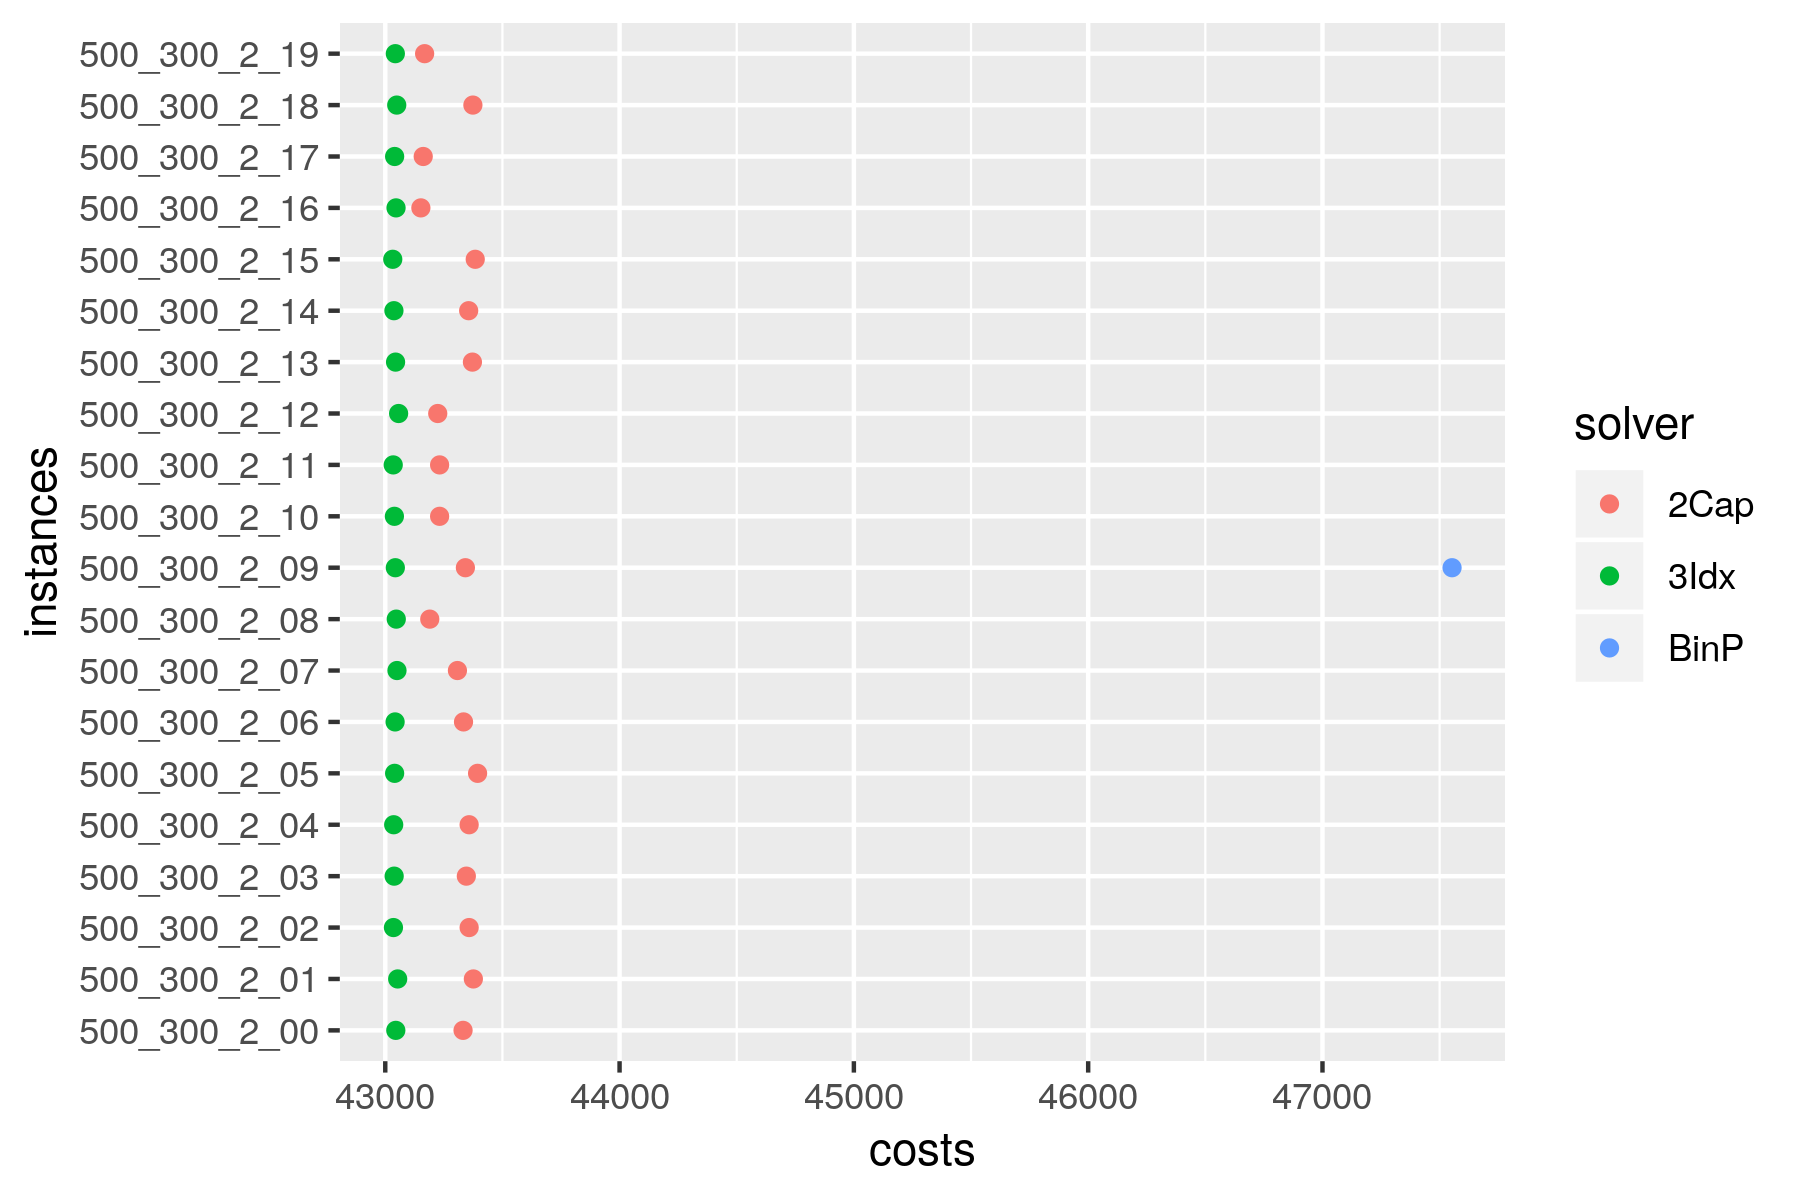
\includegraphics[width=1.3\textwidth]{img/solver_instance_cost_b=2_l_2700s.png}
\caption{\textsc{Kosten bei $45min$ Limit}}
\label{fig:b=2_l_costs}
\end{subfigure}
\caption{}
\label{fig:res_plots_b=2_l}
\end{figure}

In Abb. \ref{fig:res_b=2_l} sind die exakten Ergebnisse der MIP-Formulierungen aufgeführt, denen man
entnehmen kann, dass die 3-Index-Formulierung mit einer durchschnittlichen Laufzeit von ca. $20$ Minuten sämtliche Instanzen
optimal löst (vgl. Abb. \ref{fig:res_b=2_l_c}). Die Heuristik benötigt allerdings nur durchschnittlich $0.7s$ pro Instanz und
weicht auch nur um im Durchschnitt $0.6 \%$ vom Optimalwert ab. Dieser, verglichen mit der Kategorie der mittelgroßen Instanzen,
noch gravierende Laufzeitunterschied und die nur sehr geringe Abweichung vom Optimum sorgen dafür, dass die Heuristik in der Praxis,
wenn geringe Abweichungen gestattet sind, klar bevorzugt werden sollte.

\begin{figure}[H]
\begin{subfigure}[b]{0.3\textwidth}
\centering
\resizebox{\textwidth}{!}{
\begin{tabular}{ | l | l | l |}
    \hline
     & \textbf{BinP} & \textbf{3Idx} \\ \hline
    \textbf{Optimal} & $ \textcolor{red}{0 \%}$ & $ \textcolor{mygreen}{70 \%}$ \\ \hline
    \textbf{Laufzeit} & \textcolor{red}{$---$} & \O $\thinspace \textcolor{mygreen}{728.0 s}$ \\ \hline
    \textbf{Abweichung} & \textcolor{red}{$---$} & \O $\thinspace \textcolor{mygreen}{0.53 \%}$ \\ \hline
\end{tabular}}
\caption{\textsc{Zeitlimit} $15min$}
\label{fig:res_b=2_l_a}
\end{subfigure}
\begin{subfigure}[b]{0.3\textwidth}
\centering
\resizebox{\textwidth}{!}{
\begin{tabular}{ | l | l | l |}
    \hline
     & \textbf{BinP} & \textbf{3Idx} \\ \hline
    \textbf{Optimal} & $ \textcolor{red}{0 \%}$ & $ \textcolor{mygreen}{85 \%}$ \\ \hline
    \textbf{Laufzeit} & \textcolor{red}{$---$} & \O $\thinspace \textcolor{mygreen}{977.2 s}$ \\ \hline
    \textbf{Abweichung} & \textcolor{red}{$---$} & \O $\thinspace \textcolor{mygreen}{0.0 \%}$ \\ \hline
\end{tabular}}
\caption{\textsc{Zeitlimit} $30min$}
\label{fig:res_b=2_l_b}
\end{subfigure}
% $\quad\quad\quad\quad$
\begin{subfigure}[b]{0.3\textwidth}
\centering
\resizebox{\textwidth}{!}{
\begin{tabular}{ | l | l | l |}
    \hline
     & \textbf{BinP} & \textbf{3Idx} \\ \hline
    \textbf{Optimal} & $ \textcolor{red}{0 \%}$ & $ \textcolor{mygreen}{100 \%}$ \\ \hline
    \textbf{Laufzeit} & \textcolor{red}{$---$} & \O $\thinspace \textcolor{mygreen}{1185.9  s}$ \\ \hline
    \textbf{Abweichung} & \textcolor{red}{$---$} & \O $\thinspace \textcolor{mygreen}{0.0 \%}$ \\ \hline
\end{tabular}}
\caption{\textsc{Zeitlimit} $45min$}
\label{fig:res_b=2_l_c}
\end{subfigure}

\caption{\textsc{MIP-Ergebnisse}}
\label{fig:res_b=2_l}
\end{figure}

\textbf{Fazit}

Insgesamt ist festzuhalten, dass bei Stacking-Problemen mit Stacks der Kapazität $b = 2$ in der Kategorie der kleinen Instanzen
aufgrund der geringen Laufzeit der MIP-Formulierungen kein wirklicher Bedarf für eine Laufzeitverbesserung besteht.
Anders in den Kategorien der mittelgroßen und großen Instanzen, bei welchen die Heuristik bei nur kleinen Abweichungen zu einer
derart großen Laufzeiteinparung führt, dass sie eine in der Praxis relevante Alternative darstellt.

\subsection{Konstruktive Heuristik ($b = 3$)}
\label{sec:three_cap_heuristic}

Die konstruktive Heuristik zur Lösung von Stacking-Problemen mit Stacks der Kapazität $b = 3$ funktioniert
an einigen Stellen analog zur Heuristik aus Abschnitt \ref{sec:two_cap_heuristic} für eine Stack-Kapazität von $b = 2$.
Um den zusätzlichen Möglichkeiten und Anforderungen der erhöhten Stack-Kapazität gerecht zu werden, werden überdies
erweiternde Ansätze präsentiert.

Zunächst geht es wie auch in der Heuristik für $b = 2$ darum, kompatible Item-Paare zu bilden. Dazu wird ein
Stacking-Constraint-Graph $G = (V, E)$ generiert, welcher die Items als Knoten enthält, d.h. $V = I$.
Dieser Graph besitzt eine Kante $\{i, j\} \in E$ zwischen zwei Knoten, wenn die entsprechenden Items $i, j \in I$
basierend auf den Stacking-Constraints in mindestens einer Richtung stackbar sind, d.h. wenn $s_{ij} + s_{ji} \geq 1$
und wenn mindestens ein Stack existiert, in welchem die beiden Items gemeinsam platziert werden können ohne die Placement-Constraints
zu verletzen, also wenn $c_{iq} < \infty$ und $c_{jq} < \infty$ für mindestens einen Stack $q \in Q$ gilt.

Berechnet man nun ein \textsc{MCM} $M \subseteq E$ in $G$ und interpretiert dessen Kanten $\{i, j\} \in M$ als Paare von kompatiblen Items
$i, j \in I$, so erhält man eine größtmögliche Anzahl von Item-Paaren, die in mindestens einer Richtung stackbar sind. In der Regel ist es möglich, dass dabei sämtliche Items einer Instanz Teil eines Paares sind, denn typischerweise ist die Anzahl der Items gerade.
Dies hängt allerdings zusätzlich von den gegebenen Stacking-Constraints ab und gilt nur für die zweite Variante der Stacking-Constraint-Generierung, welche in Kapitel \ref{sec:test_data} beschrieben wird. Da diese jedoch realitätsnäher zu sein scheint und daher auch in sämtlichen Experimenten zum Einsatz kommt, ist davon auszugehen, dass an dieser Stelle keine Unmatched-Items verbleiben.
Dieser Sachverhalt hat dazu geführt, dass sich die weitere Berechnung eines \textsc{MCM} zwischen Item-Paaren und Unmatched-Items,
um erste Tripel zu bilden, welche in einer früheren Version der Heuristik an dieser Stelle stattfand, als nicht zielführend
erwies.

Da die Stacks nun nicht nur Paare, sondern Tripel von Items beinhalten können, geht es im Folgenden darum,
ebensolche Tripel von kompatiblen Items zu generieren. Dazu werden die zuvor gebildeten Item-Paare zu Item-Tripeln gemergt.
Zunächst muss allerdings entschieden werden, welche dieser Paare sinnvollerweise wieder separiert werden sollten,
um beide Items einem jeweils anderen Paar zuzuweisen und zwei Tripel zu bilden. Dies geschieht mithilfe eines Rating-Systems, welches die Item-Paare mit dem Ziel bewertet, jene Paare zu ermitteln, die im Hinblick auf ein günstiges Ergebnis
und möglichst vollständig gefüllte Stacks getrennt werden sollten.

\textbf{Rating-System}

Initial wird jede Kante $\{i, j\} \in M$, also jedes Item-Paar, mit dem Basis-Rating $0$ bewertet.
Anschließend wird für jedes dieser Paare die Kompatibilität seiner Items $i, j \in I$ zu anderen Paaren aus $M \textbackslash \{i, j\}$ ermittelt.
Dementsprechend wird für jedes Item, welches Teil eines Paares ist, die Anzahl der verbleibenden Paare bestimmt, zu denen es kompatibel ist, denen es also zugewiesen werden kann, um ein Tripel zu bilden. Diese Kompatibilität bezieht sich auf die Stacking-Constraints.
Eine Menge von Items ist zueinander kompatibel, wenn diese basierend auf den Stacking-Constraints in mindestens einer
Reihenfolge gestapelt werden kann.

Geht es beispielsweise darum, zu überprüfen, ob ein Item $i \in I$ einem Paar $(s, t)$, welches aus einer Kante $\{s, t\} \in M$ resultiert,
zugewiesen werden kann, so ergeben sich die in Abb. \ref{fig:triple_permutations} dargestellten $3!$ möglichen Permutationen eines Tripels. Stellt sich eine dieser Permutationen als konform mit den Stacking-Constraints heraus, so kann das Item $i$ zusammen mit dem Paar $(s, t)$ ein zulässiges Tripel bilden.
\begin{figure}[H]
\[
\begin{bmatrix}
  \boldsymbol{i} & s & s & \boldsymbol{i} & t & t \\
  s & \boldsymbol{i} & t & t & \boldsymbol{i} & s \\
  t & t & \boldsymbol{i} & s & s & \boldsymbol{i}
\end{bmatrix}
\]
\caption{\textsc{Item-Tripel Permutationen.}}
\label{fig:triple_permutations}
\end{figure}
Sind die Items $s, t \in I$, welche das betrachtete Paar bilden, in beide Richtungen stackbar, also $s_{st} + s_{ts} = 2$, so sind sämtliche
Permutationen zu überprüfen.
Aufgrund der Transitivität der Stacking-Constraints ist das Item $i$ in diesem Fall allerdings bereits dann kompatibel zum Paar $(s, t)$,
wenn $s_{is} + s_{it} + s_{si} + s_{ti} \geq 1$ gilt.
Darf Item $s$ auf Item $t$ gestapelt werden, jedoch nicht andersherum, also $s_{st} = 1$ und $s_{ts} = 0$,
so müssen die ersten drei Permutationen überprüft werden. Item $i$ ist dann kompatibel zum Paar $(s, t)$,
wenn $s_{is} + s_{ti} \geq 1$ oder $s_{si} + s_{it} = 2$ gilt.
Gilt umgekehrt, dass lediglich Item $t$ auf Item $s$ gestapelt werden darf, also $s_{st} = 0$ und $s_{ts} = 1$, so
müssen die letzten drei Permutationen überprüft werden und Item $i$ ist kompatibel zum Paar $(s, t)$,
wenn $s_{it} + s_{si} \geq 1$ oder $s_{ti} + s_{is} = 2$ gilt.\newline
Auf diese Weise wird die Kompatibilität sämtlicher Items, welche Teil eines Paares sind, zu den verbleibenden Paaren bestimmt.
Ausschlaggebend ist dabei jeweils die Anzahl der kompatiblen Paare des weniger kompatiblen Items eines Paares,
da stets beide Items erneut zugewiesen werden müssen. Diese wird im Folgenden als \textquote{Worst-Compatibility}
$w_{ij}$ des Items $(i, j)$ bezeichnet.

Des Weiteren werden für jedes Item-Paar $(i, j)$ die durchschnittlichen Kosten einer gemeinsamen Stack-Zuweisung berechnet.
Zu diesem Zweck werden zunächst die durchschnittlichen Kosten $a$ einer zulässigen Zuweisung eines Items zu einem Stack berechnet,
also der Durchschnitt aller Einträge $c_{iq}$ für Items $i \in I$ und Stacks $q \in Q$ in der Transportkostenmatrix $C$, für
welche $t_{iq} = 1$ gilt. Dabei entspricht $c_{(i, j)q}$ jeweils den Kosten der gemeinsamen Zuweisung der Items $i$ und $j$ zu Stack $q$,
welche wie folgt definiert sind:
\[
    c_{(i, j)q} \quad := \quad
\begin{cases}
    c_{iq} + c_{jq}, & \text{wenn $t_{iq} = 1$ und $t_{jq} = 1$}\\
    5a, & \text{sonst}
\end{cases}
\]
D.h. die Kosten der Zuweisung entsprechen nur dann der Summe der beiden Einzelzuweisungen, wenn beide Items des Paares basierend
auf den Placement-Constraints kompatibel zum Stack sind. Ist dies nicht der Fall, so wird die Inkompatibilität durch
einen Kostenwert von $5a$, also dem $5$-fachen der Kosten einer durchschnittlichen Item-Stack-Zuweisung, bestraft. Der durchschnittliche Kostenwert $avgC_{ij}$ für das Item-Paar $(i, j)$ ergibt sich folgendermaßen:
\[ avgC_{ij} = \frac{\sum_{q \in Q} (c_{(i, j)q})}{|Q|}  \]

Anschließend wird über sämtliche Paare, die sich aus den Kanten $\{i, j\} \in M$ ergeben, hinweg eine durchschnittliche \textquote{Worst-Compatibility} $w$, also eine durchschnittliche Kompatibilität des jeweils weniger kompatiblen Items, sowie ein durchschnittlicher Kostenwert $avgC$ für Stackzuweisungen berechnet. Wenn ein Paar $(i, j)$ nun sowohl eine über dem Durchschnitt liegende \textquote{Worst-Compatibility} $w_{ij} > w$ als auch einen über dem Durchschnitt liegenden durchschnittlichen Kostenwert $avgC_{ij} > avgC$ besitzt, scheint es gut geeignet für eine Separation,
denn es ist überdurchschnittlich flexibel für eine erneute Zuweisung und seine gegenwärtige Zuweisung ist ohnehin überdurchschnittlich teuer.
Dabei ist selbstverständlich nicht garantiert, dass für diese Items nach der Trennung eine günstigere Zuweisung existiert.

Wenn die Summe der prozentualen Abweichungen $d_{ij}$ beider Werte des Paares $(i, j)$ vom Durchschnitt einen gewissen Schwellenwert,
welcher im Folgenden als \textquote{Deviation-Threshold} $d_t$ bezeichnet wird,
überschreitet, entspricht das Rating $r_{ij}$ des Paares ebendieser Summe.
Die Summe der prozentualen Abweichungen $d_{ij}$ ist wie folgt definiert:
\[ d_{ij} = \frac{|avgC - avgC_{ij}|}{avgC \cdot 100} + \frac{|w - w_{ij}|}{w \cdot 100}\]
Das Rating $r_{ij}$ des Paares $(i, j)$ ergibt sich dementsprechend folgendermaßen:
\[
    r_{ij} \quad := \quad
\begin{cases}
    d_{ij}, & \text{wenn $d_{ij} > d_t$}\\
    0, & \text{sonst}
\end{cases}
\]
Die Tatsache, dass das Rating $r_{ij}$ eines Paares $(i, j)$ direkt der Summe seiner Abweichungen $d_{ij}$
vom Durchschnitt entspricht, sofern diese den Schwellenwert $d_t$ überschreitet, hat zur Folge, dass die Höhe der Abweichungen
einen Einfluss auf die Bewertung der Paare hat.

Der \textquote{Deviation-Threshold} $d_t$ wird dabei in einem bestimmten Wertebereich variiert, d.h. der Prozess wird mit
unterschiedlichen Schwellenwerten durchgeführt, die zu unterschiedlich bewerteten Listen der Item-Paare führen.
Dieser Wertebereich wurde experimentell bestimmt und reicht von $d_t = 65 \%$ bis $d_t = 120 \%$ Abweichung in der Summe.
Dabei wird $d_t$ in jeder Iteration um $5 \%$ inkrementiert. Es entstehen demnach $12$ unterschiedlich bewertete Itemlisten zusätzlich zum ursprünglichen Ergebnis des \textsc{MCM}, welches unbeweret und unsortiert betrachtet wird. Diese Listen werden absteigend basierend auf ihrer Bewertung sortiert.

Da die Verwendung des beschriebenen Rating-Systems zu einer durchaus signifikanten Laufzeitverlängerung führt,
wird in der Implementation der Heuristik ein Parameter \textit{prioritizeRuntime} eingeführt, welcher ein Deaktivieren des
Rating-Systems ermöglicht, um eine möglichst geringe Laufzeit zu gewährleisten. Wird dieser Parameter auf \textit{true}
gesetzt, so wird das initiale Ergebnis des \textsc{MCM} als einzige Liste von Item-Paaren im Merge-Prozess verwendet und
resultiert schließlich auch nur in einer einzigen Lösung.
Wird das Rating-System verwendet, so erhöht sich die durchschnittliche Laufzeit pro Instanz in der Kategorie der großen
Instanzen, in welcher es die größte Auswirkung auf die Laufzeiten zeigt, von $0.5 s$ auf $4.2 s$. Dabei verringert
sich der Zielfunktionswert in den unterschiedlichen Kategorien um durchschnittlich $0.007 \% (l), 0.04 \% (m)$
und $0.13 \% (s)$. Trotz der vergleichsweise geringen Verbesserungen der Zielfunktionswerte im Durchschnitt,
ist diese im Einzelfall durchaus relevant. Gerade in Anbetracht der ohnehin bereits geringen Abweichung der Heuristik vom Optimum,
kann diese jenem durch Verwendung des Rating-Systems noch einmal näher kommen. Wenn also eine Laufzeit von wenigen Sekunden, welche
die MIP-Formulierungen weiterhin um Größenordnungen unterbietet, akzeptabel ist, sollte dies in Betracht gezogen werden.

Nachdem die unterschiedlich sortierten Listen generiert wurden, geht es um den tatsächlichen Merge-Prozess.
Die ersten $x$ Paare einer Liste werden separiert, was den ersten $x$ Paaren mit dem höchsten Rating, also der größten
prozentualen Abweichung vom Durchschnitt in der Summe $d_{ij}$ entspricht. Die daraus resultierenden einzelnen Items werden den verbleibenden
$|M| - x$ Paaren zugewiesen um kompatible Tripel zu bilden. Die größte Anzahl an Item-Paaren, die separiert und dessen Items theoretisch den verbleibenden Paaren zugewiesen werden könnten, beträgt $\floor{\frac{|M|}{3}}$. Aufgrund der Stacking Constraints ist es jedoch nicht sinnvoll, die Minimalanzahl verbleibender Paare zu wählen. Dementsprechend sollte $|M|$ durch einen Wert $> 3$ dividiert werden. Gleichzeitig sollte der Wert nicht zu groß gewählt werden, damit möglichst viele Tripel entstehen. Experimentell hat sich $3.4$ als guter Divisor herausgestellt, indem die Lösungen für unterschiedliche $x$ Werte verglichen wurden. Folglich werden die ersten $x = \floor{\frac{|M|}{3.4}}$ Paare separiert.

Nun sollen aus den dabei entstehenden Items zusammen mit den verbleibenden Paaren zulässige Tripel entstehen.
Dazu wird ein bipartiter Graph $G_1 = (V_1 \cup V_2, E_1)$ bestehend aus den Paaren und separierten Items generiert.
Dieser Graph enthält die Paare in der Partition $V_1$ und die separierten Items in der Partition $V_2$.
Es existiert eine Kante zwischen einem Paar $(i, j) \in V_1$ und einem Item $k \in V_2$, wenn das Item $k$ kompatibel zum Paar
$(i, j)$ ist. Die Überprüfung dieser Kompatibilität findet erneut in geschilderter Weise basierend auf den möglichen Permutationen
aus Abb. \ref{fig:triple_permutations} statt.

Anschließend wird in $G_1$ ein \textsc{MCM} berechnet, dessen Kanten einer größtmöglichen Menge an kompatiblen Item-Tripeln entspricht.
Dies geschieht für sämtliche Listen von Item-Paaren basierend auf den unterschiedlichen Sortierungen.
Daraufhin liegt also eine Menge von Listen von Item-Tripeln vor, die aus den unterschiedlich sortierten Listen von Item-Paaren resultiert.
Für jede dieser Listen wird nun der folgende Prozess durchgeführt.

Zunächst werden abermals durch ein \textsc{MCM} in dem für alle verbleibenden Items generierten Stacking-Constraint-Graphen
Paare gebildet, da im Zuge des Merge-Prozesses Unmatched-Items entstehen können, die nicht Teil eines Tripels sind und auch nicht notwendigerweise
sämtliche Items zuvor Teil eines Paares waren. Items, welche nicht inzident zu einer Kante dieses Matchings sind, werden im Folgenden als unmatched betrachtet und auf dem Ground-Level eines eigenen Stacks platziert.

Wie bereits in der Heuristik aus Abschnitt \ref{sec:two_cap_heuristic} werden auch hier auf diese Weise insgesamt möglichst wenige der zur Verfügung stehenden Stacks verwendet, denn wie zuvor ist das primäre Ziel, zu einer zulässigen Lösung zu gelangen, wofür sich die initiale Maximierung der Anzahl der möglichst weit gefüllten Stacks anbietet. Erst nachdem möglichst viele Tripel und Paare von Items generiert wurden, geht es darum, diese zusammen mit den verbleibenden Unmatched-Items möglichst günstig den vorhandenen Stacks zuzuweisen.

An dieser Stelle liegt also eine Menge an Item-Tripeln, eine Menge an Item-Paaren und eine Menge an Unmatched-Items vor. Diese müssen nun
noch in einer die Placement-Constraints respektierenden Weise den Stacks zugewiesen werden.
Dies ist nur dann möglich, wenn die Anzahl der Tripel, Paare und Unmatched-Items in der Summe kleiner oder gleich der Anzahl
der zur Verfügung stehenden Stacks ist.

Ist dies der Fall, so wird zu diesem Zweck ein bipartiter Graph $G_2 = (V_3 \cup V_4, E_2)$ eingeführt,
dessen erste Partition $V_3$ die Items bestehend aus Item-Tripeln, Item-Paaren und Unmatched-Items enthält während die zweite Partition $V_4$
die zur Verfügung stehenden Stacks beinhaltet. Da diese Partitionen nicht notwendigerweise dieselbe Kardinalität besitzen, der von \textit{JGrpahT} bereitgestellte Algorithmus, welcher zur Berechnung eines \textsc{MWPM} in $G_2$ verwendet wird, dies jedoch fordert, werden Dummy-Items
eingeführt, die die Item-Partition $V_3$ gegebenenfalls auffüllen.


Eine Kante $\{i, q\} \in E_2$ zwischen einem Knoten $i \in V_3$ und einem Knoten $q \in V_4$ gibt an, dass das entsprechende Item, Item-Paar oder Item-Tripel $i$ dem jeweiligen Stack $q$ zugeordnet werden kann. Wie zuvor gilt dabei
aus genannten Gründen, dass die Placement-Constraints indirekt durch ein hohes Gewicht einer solchen Kante und nicht durch ein Fehlen dieser
umgesetzt werden. Es existieren daher Kanten zwischen sämtlichen Knoten aus $V_3$ und denen aus $V_4$, d.h. $\forall i \in V_3, q \in V_4
\thinspace \exists \thinspace \{i, q\} \in E_2$, was dafür sorgt, dass es sich bei $G_2$ um einen vollständig bipartiten Graphen handelt.
Das Gewicht einer solchen Kante $\{i, q\} \in E_2$, die ein Tripel, Paar oder Unmatched-Item mit einem Stack verbindet, ist definiert
als die Summe der Kosten des Transports aller an der Zuweisung beteiligten Items zum jeweiligen Stack. Somit ergeben sich drei Fälle.
Der erste Fall behandelt Kanten $\{i, q\} \in E_2$, die ein Unmatched-Item $i \in V_3$ mit einem Stack $q \in V_4$ verbinden.
Das Gewicht einer solchen Kante entspricht den Kosten des Transports $c_{iq}$ des Items $i$ in den Stack $q$.
Fall zwei behandelt Kanten $\{(i, j), q\} \in E_2$, welche ein Item-Paar $(i, j) \in V_3$ mit einem Stack $q \in V_4$
verbinden. Die Kosten einer solchen Kante ergeben sich aus der Summe der Kosten des Transports beider Items,
also $c_{(i, j)q} = c_{iq} + c_{jq}$.
Der dritte und letzte Fall behandelt Kanten $\{(i, j, k), q\} \in E_2$, welche ein Item-Tripel $(i, j, k) \in V_3$
mit einem Stack $q \in V_4$ verbinden. Die Kosten einer solchen Kante ergeben sich aus der Summe der Kosten des Transports
der drei Items, also $c_{(i, j, k)q} = c_{iq} + c_{jq} + c_{kq}$.

Die Dummy-Items haben keinen Einfluss auf die Lösung, da sämtliche Kanten, die ein Dummy-Item mit einem Stack verbinden,
das Gewicht $0$ besitzen und somit keine günstigere Zuweisung eines echten Items, Item-Paars oder Item-Tripels durch ein Dummy-Item
verhindert wird. Diese Tatsache ergibt sich daraus, dass die Dummy-Items jedem Stack zu den Kosten $0$ zugewiesen werden können,
während eine Zuweisung echter Items, Item-Paare und Item-Tripel stets Kosten verursacht. Dementsprechend werden echte Items bei der
Zuweisung gewissermaßen bevorzugt während Dummy-Items schlicht den verbleibenden Stacks zugewiesen werden.

Nachdem beide Partitionen dieselbe Größe besitzen, wird ein \textsc{MWPM} in $G_2$ berechnet, dessen Kanten
als Stack-Zuweisungen interpretiert werden. Da es sich um ein Perfect-Matching handelt, werden sämtliche Items, Item-Paare
und Item-Tripel einem Stack zugewiesen. Die Minimum-Weight-Variante eines Perfect-Matchings sorgt dafür, dass es sich
jeweils um eine günstigste Zuweisung handelt, da die Kantenkosten jeweils den Transportkosten entsprechen.
Sollte das \textsc{MWPM} eine Kante der Kosten $\infty$ enthalten, so existiert keine zulässige Zuweisung
der generierten Tripel, Paare und Unmatched-Items zu den Stacks, welche die Placement-Constraints respektiert.

Auf diese Weise entstehen $13$ Lösungen, von denen schließlich die günstigste ausgewählt wird.
Zuletzt muss dann wiederum ggf. die Reihenfolge der Items innerhalb der Stacks so angepasst werden,
dass sie die Stacking-Constraints respektiert. Dazu werden sämtliche Stacks, denen mehr als
ein Item zugewiesen wurde, betrachtet. Für jeden dieser Stacks wird geprüft, ob die aufeinander
gestapelten Items jeweils paarweise aufeinander gestapelt sein dürfen.
Werden zwei Items innerhalb eines Stacks gefunden, welche die Stacking-Constraints verletzen, so werden diese
vertauscht und der Prozess startet für diesen Stack erneut. Ein vollständig gefüllter Stack ist mit dieser
Strategie nach spätestens drei Tausch-Operationen korrekt sortiert. Durch die bei der Zuweisung geprüfte
Kompatibilität ist sichergestellt, dass eine solche Reihenfolge existiert.

\textbf{Beispiel}

Gegeben sei die Item-Menge $I = \{0, 1, 2, 3, 4, 5, 6, 7, 8, 9, 10, 11, 12, 13\}$ sowie eine Stack-Kapazität von $b = 3$.
Die Anzahl der zur Verfügung stehenden Stacks ergibt sich, wie in Abschnitt \ref{sec:test_data} beschrieben,
durch $m = \ceil{\floor{\frac{14}{3}} + 20 \%} = 5$.

Zunächst wird, wie in Abschnitt \ref{sec:test_data} beschrieben, der Stacking-Constraint-Graph für die Item-Menge $I$ generiert,
auf welchem anschließend analog zum Beispiel aus Abschnitt \ref{sec:two_cap_heuristic} ein \textsc{MCM} berechnet wird.
In Abb. \ref{fig:item_pairs_example_b=3} ist das Ergebnis dargestellt, welches die Kanten des \textsc{MCM} interpretiert
als Item-Paare zeigt.

\begin{figure}[H]
\centering
\begin{tikzpicture}[auto, transform shape, node distance=2cm,every node/.style={draw,fill=gray!40,circle,minimum size=100000mm}]
        \node[state] (A) [thick] {$\boldsymbol{00, 01}$};
        \node[state] (B) [thick, right of=A] {$\boldsymbol{02, 05}$};
        \node[state] (C) [thick, right of=B] {$\boldsymbol{03, 04}$};
        \node[state] (D) [thick, right of=C] {$\boldsymbol{06, 07}$};
        \node[state] (E) [thick, right of=D] {$\boldsymbol{08, 09}$};
        \node[state] (F) [thick, right of=E] {$\boldsymbol{10, 11}$};
        \node[state] (G) [thick, right of=F] {$\boldsymbol{12, 13}$};
        \path;
\end{tikzpicture}
\caption{\textsc{Resultierende Item-Paare}.}
\label{fig:item_pairs_example_b=3}
\end{figure}

Anschließend geht es darum, aus den in Abb. \ref{fig:item_pairs_example_b=3} dargestellten Paaren von Items möglichst viele
Tripel von Items zu mergen. Zunächst muss allerdings basierend auf dem Rating-System entschieden werden, welche
Paare wieder separiert werden. Daraus ergeben sich die Folgenden unterschiedlich sortierten Listen von Item-Paaren:
\begin{figure}[H]
\begin{gather*}
  [(12, 13), (10, 11), (8, 9), (6, 7), (3, 4), (2, 5), (0, 1)] \\
  [(8, 9), (12, 13), (0, 1), (10, 11), (6, 7), (3, 4), (2, 5)] \\
  [(8, 9), (12, 13), (10, 11), (6, 7), (3, 4), (2, 5), (0, 1)]
\end{gather*}
\caption{\textsc{Unterschiedlich sortierte Listen der Item-Paare}.}
\label{fig:lists_of_pairs}
\end{figure}
Es ergeben sich dabei in zuvor beschriebenr Weise $13$ potenziell unterschiedlich sortierte Listen von Item-Paaren.
In diesem Fall ergeben sich u.a. aufgrund der geringen Anzahl an Paaren jedoch lediglich drei voneinander unterschiedliche
Sortierungen (vgl. Abb. \ref{fig:lists_of_pairs}).

\pagebreak

Nun geht es darum, die ersten $\floor{\frac{7}{3.4}} = 2$ Paare zu separieren und möglichst sämtliche der dabei entstehenden
Items den verbleibenden Paaren zuzuweisen. Für die erste der drei unterschiedlichen Sortierungen ergibt sich
die in Abb. \ref{fig:pre_merge_step} dargestellte Aufteilung in Paare, welche separiert werden (vgl. Abb. \ref{fig:split_pairs})
und jene, denen die daraus resultierenden Items zugewiesen werden um Item-Tripel zu bilden (vgl. Abb. \ref{fig:assign_pairs}).

\begin{figure}[H]
\centering
\begin{subfigure}[b]{\textwidth}
\centering
\begin{tikzpicture}[scale=0.85, transform shape, node distance=2cm]
        \node[state] (A) [thick] {$\boldsymbol{12, 13}$};
        \node[state] (B) [thick, right of=A] {$\boldsymbol{10, 11}$};
        \path;
\end{tikzpicture}
\caption{\textsc{Split-Pairs}.}
\label{fig:split_pairs}
\end{subfigure}
\begin{subfigure}[b]{\textwidth}
\centering
\begin{tikzpicture}[scale=0.85, transform shape, node distance=2cm]
        \node[state] (A) [thick] {$\boldsymbol{08, 09}$};
        \node[state] (B) [thick, right of=A] {$\boldsymbol{06, 07}$};
        \node[state] (C) [thick, right of=B] {$\boldsymbol{03, 04}$};
        \node[state] (D) [thick, right of=C] {$\boldsymbol{02, 05}$};
        \node[state] (E) [thick, right of=D] {$\boldsymbol{00, 01}$};
        \path;
\end{tikzpicture}
\caption{\textsc{Assign-Pairs}.}
\label{fig:assign_pairs}
\end{subfigure}
\caption{\textsc{Merge Vorbereitung}.}
\label{fig:pre_merge_step}
\end{figure}

Anschließend wird der in Abb. \ref{fig:bipartite_graph_pairs_and_unmatched} dargestellte bipartite Graph generiert,
welcher die Paare in der einen Partition und die einzelnen Items, welche aus der Separation der Paare in Abb. \ref{fig:split_pairs} resultieren, in der anderen Partition enthält. Eine Kante zwischen einem einzelnen Item und einem Paar bedeutet,
dass dieses Item dem Paar zugeordnet werden kann, sodass ein kompatibles Tripel entsteht.
In Abb. \ref{fig:item_triple_mcm} ist das auf diesem Graphen berechnete \textsc{MCM} in grün dargestellt, in welchem
sämtliche einzelnen Items einem Paar zugewiesen werden. Das Paar $(2, 5)$ wird dabei als einziges Paar nicht verwendet
und verbleibt dementsprechend als Item-Paar.

\begin{figure}[H]
\centering

\begin{subfigure}[b]{0.4\textwidth}
\centering
\begin{tikzpicture}[scale=0.85, transform shape, node distance=2cm]
        \node[state] (A) [thick] {$\boldsymbol{8, 9}$};
        \node[state] (B) [thick, below of=A] {$\boldsymbol{6, 7}$};
        \node[state] (C) [thick, below of=B] {$\boldsymbol{3, 4}$};
        \node[state] (D) [thick, below of =C] {$\boldsymbol{2, 5}$};
        \node[state] (E) [thick, below of=D] {$\boldsymbol{0, 1}$};
        \node[state] (F) [thick, right = 4cm of A] {$\boldsymbol{12}$};
        \node[state] (G) [thick, below of=F] {$\boldsymbol{13}$};
        \node[state] (H) [thick, below of=G] {$\boldsymbol{10}$};
        \node[state] (I) [thick, below of=H] {$\boldsymbol{11}$};
        \path
          (A) edge [thick] node {} (F)
          (A) edge [thick] node {} (G)
          (A) edge [thick] node {} (H)
          (A) edge [thick] node {} (I)

          (B) edge [thick] node {} (F)
          (B) edge [thick] node {} (H)

          (C) edge [thick] node {} (F)
          (C) edge [thick] node {} (G)
          (C) edge [thick] node {} (H)

          (D) edge [thick] node {} (F)
          (D) edge [thick] node {} (H)

          (E) edge [thick] node {} (F)
          (E) edge [thick] node {} (G)
          (E) edge [thick] node {} (H)
          (E) edge [thick] node {} (I);
\end{tikzpicture}
\caption{\textsc{Bipartiter Graph}.}
\label{fig:bipartite_graph_pairs_and_unmatched}
\end{subfigure}
\hspace{10pt}
\begin{subfigure}[b]{0.4\textwidth}
\centering
\begin{tikzpicture}[scale=0.85, transform shape, node distance=2cm]
        \node[state] (A) [thick] {$\boldsymbol{\textcolor{mygreen}{8, 9}}$};
        \node[state] (B) [thick, below of=A] {$\boldsymbol{\textcolor{mygreen}{6, 7}}$};
        \node[state] (C) [thick, below of=B] {$\boldsymbol{\textcolor{mygreen}{3, 4}}$};
        \node[state] (D) [thick, below of =C] {$\boldsymbol{\textcolor{red}{2, 5}}$};
        \node[state] (E) [thick, below of=D] {$\boldsymbol{\textcolor{mygreen}{0, 1}}$};
        \node[state] (F) [thick, right = 4cm of A] {$\boldsymbol{\textcolor{mygreen}{12}}$};
        \node[state] (G) [thick, below of=F] {$\boldsymbol{\textcolor{mygreen}{13}}$};
        \node[state] (H) [thick, below of=G] {$\boldsymbol{\textcolor{mygreen}{10}}$};
        \node[state] (I) [thick, below of=H] {$\boldsymbol{\textcolor{mygreen}{11}}$};
        \path
          (A) edge [mygreen, thick] node {} (F)
          (A) edge [thick] node {} (G)
          (A) edge [thick] node {} (H)
          (A) edge [thick] node {} (I)

          (B) edge [thick] node {} (F)
          (B) edge [mygreen, thick] node {} (H)

          (C) edge [thick] node {} (F)
          (C) edge [mygreen, thick] node {} (G)
          (C) edge [thick] node {} (H)

          (D) edge [thick] node {} (F)
          (D) edge [thick] node {} (H)

          (E) edge [thick] node {} (F)
          (E) edge [thick] node {} (G)
          (E) edge [thick] node {} (H)
          (E) edge [mygreen, thick] node {} (I);
\end{tikzpicture}
\caption{\textsc{MCM}.}
\label{fig:item_triple_mcm}
\end{subfigure}

\caption{\textsc{Item-Tripel Generierung.}}
\label{fig:item_triple_generation}
\end{figure}

\pagebreak

Abbildung \ref{fig:merge_result} zeigt das Ergebnis des Merge-Prozesses, in welchem durch das
\textsc{MCM} zusätzlich zum verbleibenden Item-Paar vier Item-Tripel generiert wurden.

\begin{figure}[H]
\centering
\begin{tikzpicture}[scale=0.85, transform shape, node distance=2cm]
        \node[state] (A) [thick] {$\boldsymbol{8, 9, 12}$};
        \node[state] (B) [thick, right of=A] {$\boldsymbol{6, 7, 10}$};
        \node[state] (C) [thick, right of=B] {$\boldsymbol{3, 4, 13}$};
        \node[state] (D) [thick, right of=C] {$\boldsymbol{0, 1, 11}$};
        \node[state] (E) [thick, right of=D] {$\boldsymbol{2, 5}$};
        \path;
\end{tikzpicture}
\caption{\textsc{Merge-Ergebnis.}}
\label{fig:merge_result}
\end{figure}

Die in Abb. \ref{fig:merge_result} dargestellten Item-Tripel, sowie das Item-Paar, werden im Folgenden
möglichst günstig und in einer Weise, welche die Placement-Constraints respektiert, einem Stack zugewiesen.
Dafür wird zunächst der vollständig bipartite Graph in Abb. \ref{fig:complete_bipartite} eingeführt.
Dieser Graph enthält die Items bestehend aus vier Tripeln und einem Paar in der einen Partition
und die Stacks in der anderen. Anschließend wird ein \textsc{MWPM} in diesem Graphen berechnet, welches
in Abb. \ref{fig:mwpm} dargestellt ist.

\begin{figure}[H]
% \begin{figure}[H]
\begin{subfigure}[b]{0.4\textwidth}
\centering
\begin{tikzpicture}[scale=0.85, transform shape, node distance=2cm]
        \node[state] (A) [thick] {$\boldsymbol{8, 9, 12}$};
        \node[state] (B) [thick, below of=A] {$\boldsymbol{6, 7, 10}$};
        \node[state] (C) [thick, below of=B] {$\boldsymbol{3, 4, 13}$};
        \node[state] (D) [thick, below of=C] {$\boldsymbol{0, 1, 11}$};
        \node[state] (E) [thick, below of=D] {$\boldsymbol{2, 5}$};

        \node[state] (F) [thick, right = 4cm of A] {$\boldsymbol{S_1}$};
        \node[state] (G) [thick, below of=F] {$\boldsymbol{S_2}$};
        \node[state] (H) [thick, below of=G] {$\boldsymbol{S_3}$};
        \node[state] (I) [thick, below of=H] {$\boldsymbol{S_4}$};
        \node[state] (J) [thick, below of=I] {$\boldsymbol{S_5}$};

        \path
          (A) edge [thick] node {} (F)
          (A) edge [thick] node {} (G)
          (A) edge [thick] node {} (H)
          (A) edge [thick] node {} (I)
          (A) edge [thick] node {} (J)

          (B) edge [thick] node {} (F)
          (B) edge [thick] node {} (G)
          (B) edge [thick] node {} (H)
          (B) edge [thick] node {} (I)
          (B) edge [thick] node {} (J)

          (C) edge [thick] node {} (F)
          (C) edge [thick] node {} (G)
          (C) edge [thick] node {} (H)
          (C) edge [thick] node {} (I)
          (C) edge [thick] node {} (J)

          (D) edge [thick] node {} (F)
          (D) edge [thick] node {} (G)
          (D) edge [thick] node {} (H)
          (D) edge [thick] node {} (I)
          (D) edge [thick] node {} (J)

          (E) edge [thick] node {} (F)
          (E) edge [thick] node {} (G)
          (E) edge [thick] node {} (H)
          (E) edge [thick] node {} (I)
          (E) edge [thick] node {} (J);
\end{tikzpicture}
\caption{\textsc{Vollständig Bipartit}.}
\label{fig:complete_bipartite}
\end{subfigure}
\hfill
\begin{subfigure}[b]{0.4\textwidth}
\centering
\begin{tikzpicture}[scale=0.85, transform shape, node distance=2cm]
        \node[state] (A) [thick] {$\boldsymbol{8, 9, 12}$};
        \node[state] (B) [thick, below of=A] {$\boldsymbol{6, 7, 10}$};
        \node[state] (C) [thick, below of=B] {$\boldsymbol{3, 4, 13}$};
        \node[state] (D) [thick, below of=C] {$\boldsymbol{0, 1, 11}$};
        \node[state] (E) [thick, below of=D] {$\boldsymbol{2, 5}$};

        \node[state] (F) [thick, right = 4cm of A] {$\boldsymbol{S_1}$};
        \node[state] (G) [thick, below of=F] {$\boldsymbol{S_2}$};
        \node[state] (H) [thick, below of=G] {$\boldsymbol{S_3}$};
        \node[state] (I) [thick, below of=H] {$\boldsymbol{S_4}$};
        \node[state] (J) [thick, below of=I] {$\boldsymbol{S_5}$};

        \path
          (A) edge [thick] node {} (I)
          (B) edge [thick] node {} (F)
          (C) edge [thick] node {} (J)
          (D) edge [thick] node {} (H)
          (E) edge [thick] node {} (G);
\end{tikzpicture}
\caption{\textsc{MWPM}.}
\label{fig:mwpm}
\end{subfigure}
\caption{\textsc{Stack-Zuweisung}.}
\label{}
\end{figure}

Die Kanten des \textsc{MWPM} in Abb. \ref{fig:mwpm} werden als Stack-Zuweisungen interpretiert.
Die daraus resultierende Stacking-Lösung ist in Abb. \ref{fig:valid_solution} abgebildet. Wobei die Reihenfolge
innerhalb der Stacks ggf. in zuvor beschriebener Weise angepasst werden muss.

Diese Lösung basiert auf der ersten der drei unterschiedlichen Sortierungen aus Abb. \ref{fig:lists_of_pairs}.
Um die bestmögliche Lösung zu finden, wird der geschilderte Prozess für die beiden übrigen Sortierungen
ebenfalls durchgeführt und schließlich die beste Lösung in Bezug auf die Kosten ausgewählt.

\begin{figure}[H]
  \centering
  \resizebox{0.3\textwidth}{!}{
    \begin{tabular}{c|c|c|c|c|c|}
    \cline{2-6}
    $\boldsymbol{L_3}$ & $6$ & $$ & $0$ & $8$ & $3$ \\ \cline{2-6}
    $\boldsymbol{L_2}$ & $7$ & $2$ & $1$ & $9$ & $4$ \\ \cline{2-6}
    $\boldsymbol{L_1}$ & $10$ & $5$ & $11$ & $12$ & $13$ \\ \cline{2-6}
    \multicolumn{1}{c}{} & \multicolumn{1}{c}{$\boldsymbol{S_1}$} & \multicolumn{1}{c}{$\boldsymbol{S_2}$}
    & \multicolumn{1}{c}{$\boldsymbol{S_3}$} & \multicolumn{1}{c}{$\boldsymbol{S_4}$} & \multicolumn{1}{c}{$\boldsymbol{S_5}$} \\
    \end{tabular}}
    \caption{\textsc{Zulässige Zuweisungen.}}
    \label{fig:valid_solution}
\end{figure}

\subsection{Vergleich der $b = 3$ Solver}
\label{sec:solver_comp_b=3}

In diesem Kapitel werden die verschiedenen Solver für Instanzen von Stacking-Problemen mit einer Stack-Kapazität
von $b = 3$ miteinander verglichen. Dabei gilt weiterhin das in Kapitel \ref{sec:solver_comp_b=2} vorgestellte Setup
bezüglich der Vergleichskategorien, der \textsc{CPLEX}-Konfiguration sowie der verwendeten Hardware.

Der in Abschnitt \ref{sec:three_cap_heuristic} eingeführte Parameter \textit{prioritizeRuntime} zur Konfiguration der Heuristik
wird in den folgenden Experimenten stets auf \textit{false} gesetzt, weil die durch Verwendung des Rating-Systems erhöhten Laufzeiten
aus praktischer Perspektive vermutlich in jedem Fall vertretbar sind. Aufgrunddessen liegt der Fokus hier auf dem Erreichen
möglichst geringer Zielfunktionswerte. Liegt der Fokus in der Praxis hingegen auf einer möglichst geringen Laufzeit, so kann dementsprechend
\textit{prioritizeRuntime} auf \textit{true} gesetzt werden, was zu erheblich kürzeren Laufzeiten bei nur geringfügig schlechteren
Zielfunktionswerten führt.

\pagebreak

\textbf{Kleine Instanzen (s)}

Zunächst zum experimentellen Vergleich der Solver für in Kapitel \ref{sec:test_data} als klein definierte
Instanzen, bei denen es darum geht, 100 eintreffende Items in die Storage-Area zu verladen.

In Abb. \ref{fig:instance_coverage_b=3_s} ist die Instance-Coverage der einzelnen Solver bei einem Zeitlimit von $3, 5$
und $10$ Sekunden pro Instanz dargestellt. Die Bin-Packing-Formulierung ist hier offensichtlich schneller als die 3-Index-Formulierung.
Diese hat bereits bei einem Zeitlimit von $3s$ sämtliche Instanzen gelöst, während die 3-Index-Formulierung
bei diesem Zeitlimit lediglich drei Instanzen löst. Die Ergebnisse aus Abschnitt \ref{sec:solver_comp_b=2} in der Kategorie der kleinen
Instanzen haben sich also bezüglich der MIP-Formulierungen für eine Stack-Kapazität von $b = 3$ umgekehrt, denn in diesem Fall
ist die Bin-Packing-Formulierung der 3-Index-Formulierung vorzuziehen.

Grundsätzlich gilt, wie Abb. \ref{fig:instance_coverage_b=3_s_c} zu entnehmen ist, dass sämtliche Solver
bei einem vergleichsweise geringen Zeitlimit von $10s$ alle Instanzen lösen. Für die Heuristik ist das Zeitlimit irrelevant,
da diese mit einer durchschnittlichen Laufzeit von $0.09s$ sämtliche Instanzen löst.

\begin{figure}[H]
\centering

\begin{subfigure}[b]{0.3\textwidth}
\centering
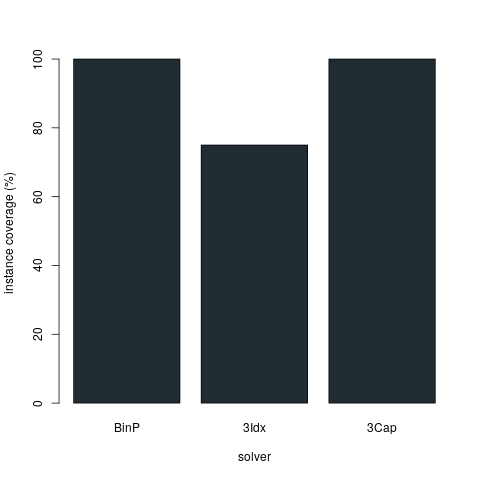
\includegraphics[width=1.2\textwidth]{img/solver_instance_coverage_b=3_s_3s.png}
\caption{\textsc{Zeitlimit} $3s$}
\label{fig:instance_coverage_b=3_s_a}
\end{subfigure}
\hfill
\begin{subfigure}[b]{0.3\textwidth}
\centering
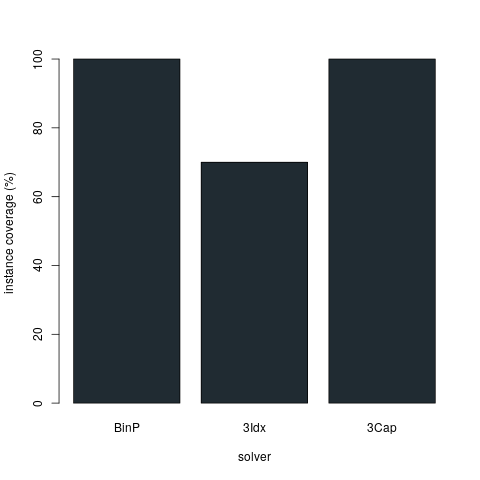
\includegraphics[width=1.2\textwidth]{img/solver_instance_coverage_b=3_s_5s.png}
\caption{\textsc{Zeitlimit} $5s$}
\label{fig:instance_coverage_b=3_s_b}
\end{subfigure}
\hfill
\begin{subfigure}[b]{0.3\textwidth}
\centering
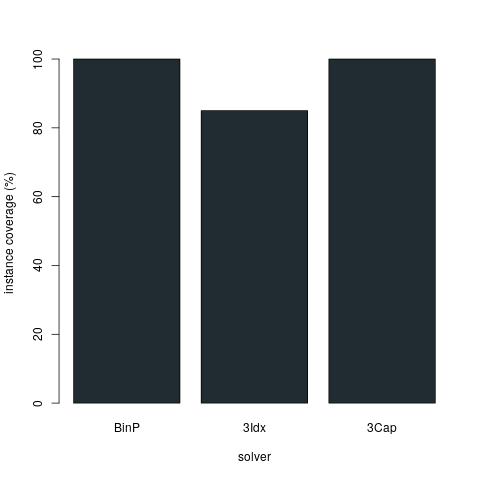
\includegraphics[width=1.2\textwidth]{img/solver_instance_coverage_b=3_s_10s.png}
\caption{\textsc{Zeitlimit} $10s$}
\label{fig:instance_coverage_b=3_s_c}
\end{subfigure}

\caption{\textsc{Instance-Coverage}.}
\label{fig:instance_coverage_b=3_s}
\end{figure}

In der Darstellung der Laufzeiten in Abb. \ref{fig:b=3_s_runtimes} ist zu erkennen, dass die Bin-Packing-
und die 3-Index-Formulierung, obwohl die Bin-Packing-Formulierunge in der Regel schneller ist,
häufig ähnliche Laufzeiten von ca. $2.5$ bis $5$ Sekunden besitzen.
Da die 3-Index-Formulierung mit den Instanzen $03, 09, 10, 11$ und $13$ allerdings einige Ausreißer,
welche eine erheblich längere Laufzeit erfordern, zeigt, ist die Bin-Packing-Formulierung im Durchschnitt klar schneller.
Die Heuristik unterbietet diese mit einer durchschnittlichen Laufzeit von nur $0.09s$ allerdings noch einmal deutlich
und weicht dabei um nur durchschnittlich $0.94 \%$ vom Optimum ab.

\pagebreak

Da die Bin-Packing-Formulierung, wie in Abb. \ref{fig:b=3_s_runtimes} zu erkennen ist, stets vor dem Zeitlimit terminiert,
löst diese sämtliche Instanzen optimal. Die 3-Index-Formulierung wird basierend auf der Abbildung in drei Fällen
durch das Zeitlimit gestoppt. Wie man in Abb. \ref{fig:b=3_s_costs} erkennen kann, wurden mit den
Instanzen $03$ und $11$ zwei jener drei Instanzen nicht optimal gelöst.
In diesen Fällen gelangt die Heuristik sogar zu besseren Zielfunktionswerten.
Im dritten Fall, in welchem die 3-Index-Formulierung durch das Zeitlimit gestoppt wurde, der Instanz $09$, hat \textsc{CPLEX}
offenkundig lediglich noch nicht bewiesen, dass es sich um das Optimum handelt, der entsprechende Wert wurde allerdings,
wie man Abb. \ref{fig:b=3_s_costs} entnehmen kann, bereits ermittelt. Sofern beide MIP-Formulierungen den Optimalwert ermittelt haben,
verdecken die Einträge der 3-Index-Formulierung in der Abb. jeweils die Einträge der Bin-Packing-Formulierung.

\begin{figure}[H]
\centering
\begin{subfigure}[b]{0.4\textwidth}
\centering
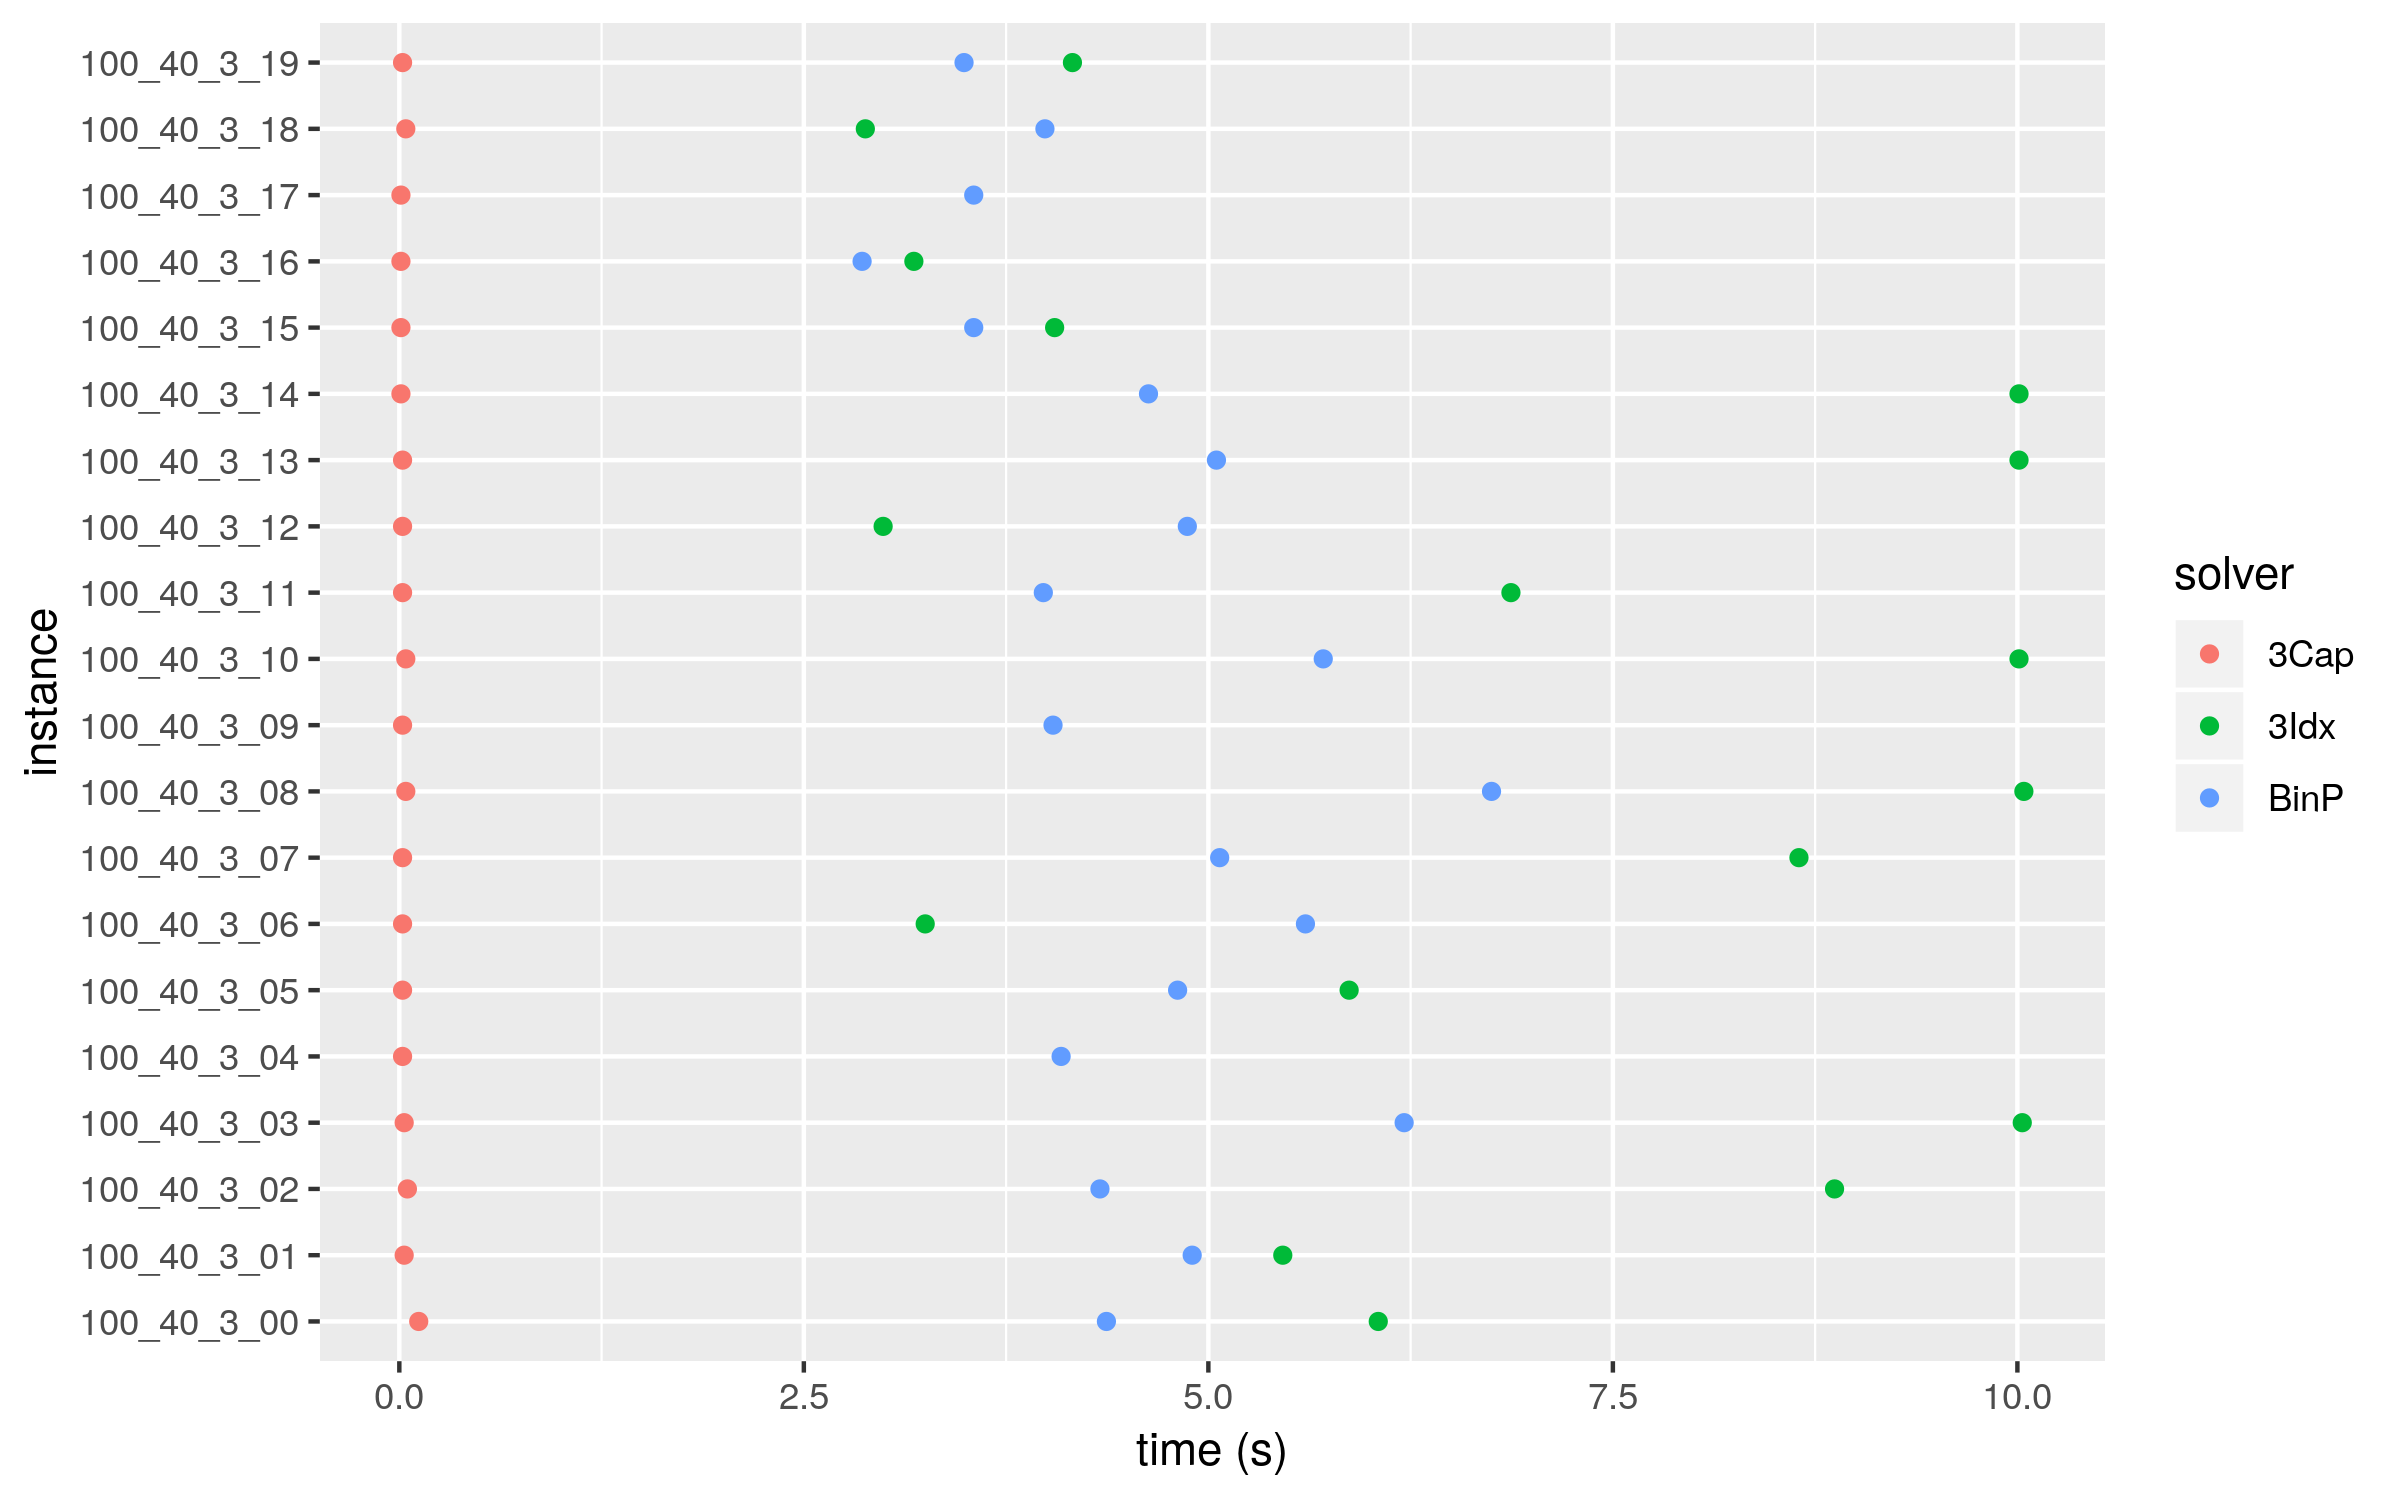
\includegraphics[width=1.3\textwidth]{img/solver_instance_time_b=3_s_10s.png}
\caption{\textsc{Laufzeiten}}
\label{fig:b=3_s_runtimes}
\end{subfigure}
\hfill
\begin{subfigure}[b]{0.4\textwidth}
\centering
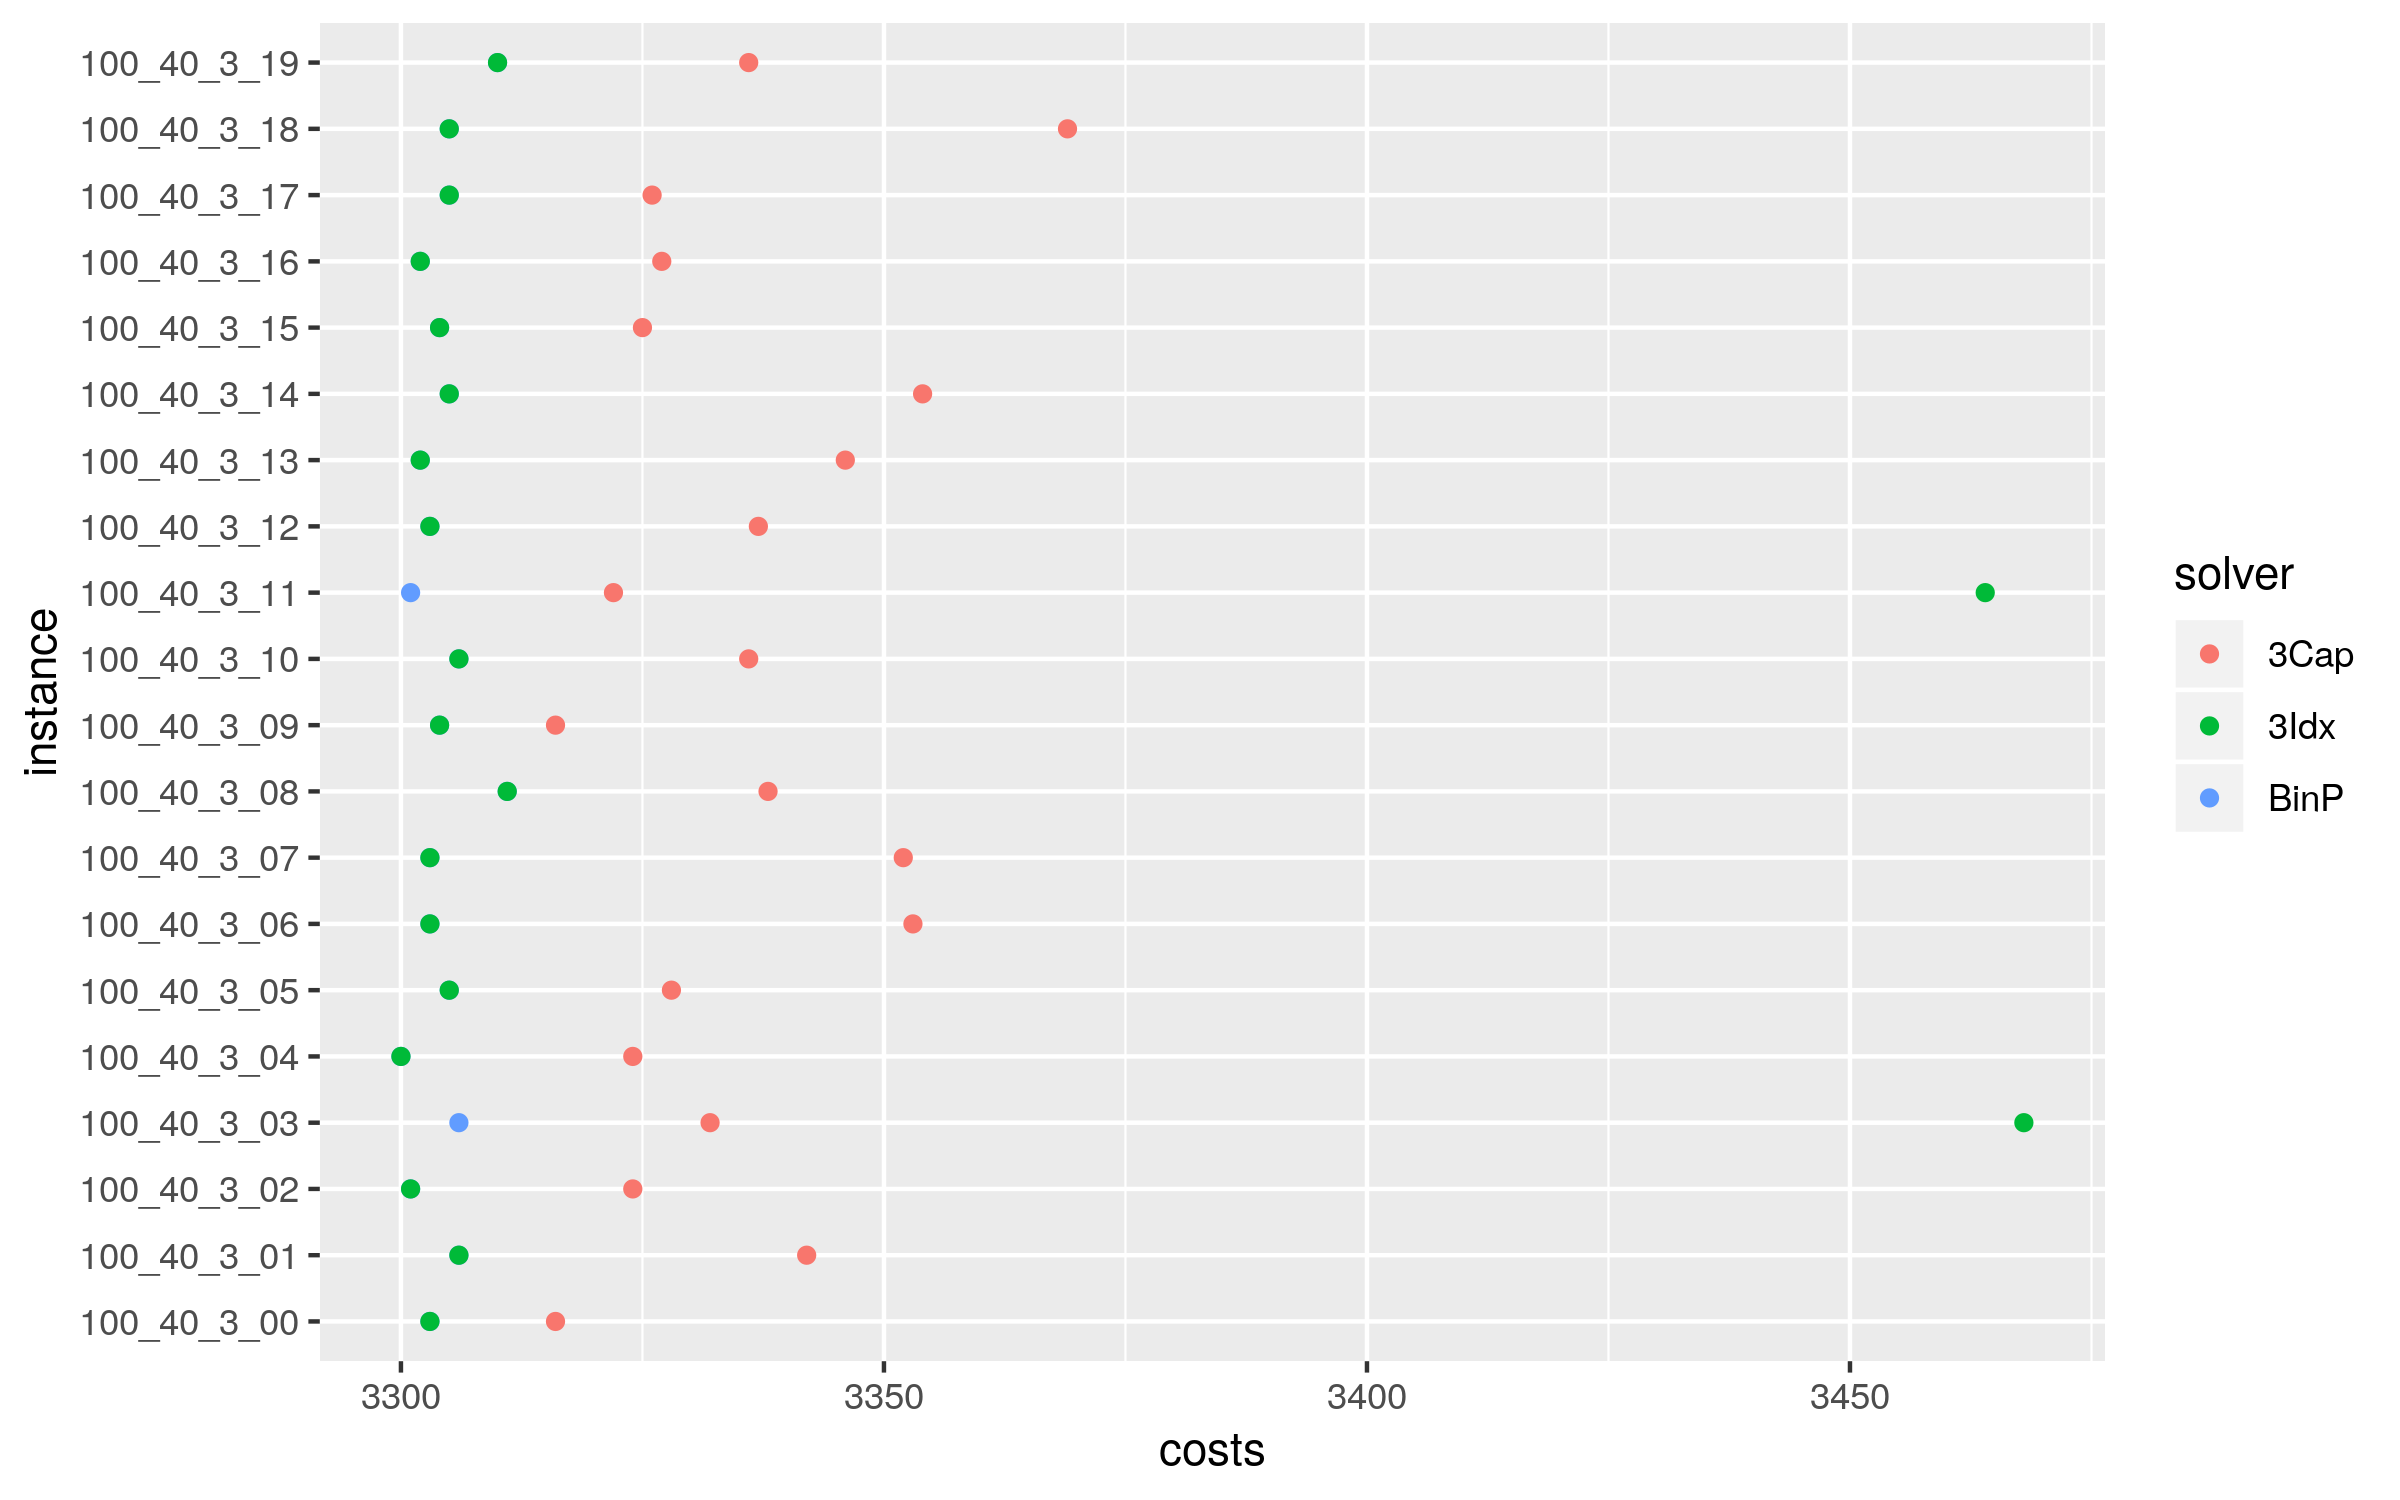
\includegraphics[width=1.3\textwidth]{img/solver_instance_cost_b=3_s_10s.png}
\caption{\textsc{Kosten}}
\label{fig:b=3_s_costs}
\end{subfigure}
\caption{\textsc{Ergebnisse bei $10s$ Zeitlimit}.}
\end{figure}

Abbildung \ref{fig:mip_results_b=3_s_b} ist zu entnehmen, dass die Bin-Packing-Formulierung nach durchschnittlich
$3.1s$ sämtliche Instanzen optimal löst. Bei einem Zeitlimit von $10s$ löst die 3-Index-Formulierung zwar ebenfalls
sämtliche Instanzen (vgl. \ref{fig:instance_coverage_b=3_s_c}), allerdings nur $90 \%$ optimal (vgl. \ref{fig:mip_results_b=3_s_c}). Dafür benötigt diese eine durchschnittliche Laufzeit von $5.9s$.
Wie bereits einleitend anhand der Instance-Coverage deutlich wurde, ist die Bin-Packing-Formulierung der 3-Index-Formulierung in dieser Kategorie vorzuziehen.

\begin{figure}[H]
\centering
\begin{subfigure}[b]{0.3\textwidth}
\centering
\resizebox{\textwidth}{!}{
\begin{tabular}{ | l | l | l |}
    \hline
     & \textbf{BinP} & \textbf{3Idx} \\ \hline
    \textbf{Optimal} & $\textcolor{mygreen}{50 \%}$ & $\textcolor{red}{5 \%}$ \\ \hline
    \textbf{Laufzeit} & \O $\thinspace 2.9 s$ & \O $\thinspace 2.9 s$ \\ \hline
    \textbf{Abweichung} & \O $\thinspace \textcolor{mygreen}{1.7 \%}$ & \O $\thinspace \textcolor{red}{7.8 \%}$ \\ \hline
\end{tabular}}
\caption{\textsc{Zeitlimit} $3s$}
\label{fig:mip_results_b=3_s_a}
\end{subfigure}
% \end{figure}
% \begin{figure}[H]
\begin{subfigure}[b]{0.3\textwidth}
\centering
\resizebox{\textwidth}{!}{
\begin{tabular}{ | l | l | l |}
    \hline
     & \textbf{BinP} & \textbf{3Idx} \\ \hline
    \textbf{Optimal} & $\textcolor{mygreen}{100 \%}$ & $\textcolor{red}{50 \%}$ \\ \hline
    \textbf{Laufzeit} & \O $\thinspace \textcolor{mygreen}{3.1 s}$ & \O $\thinspace \textcolor{red}{4.0 s}$ \\ \hline
    \textbf{Abweichung} & \O $\thinspace \textcolor{mygreen}{0 \%}$ & \O $\thinspace \textcolor{red}{1.2 \%}$ \\ \hline
\end{tabular}}
\caption{\textsc{Zeitlimit} $5s$}
\label{fig:mip_results_b=3_s_b}
\end{subfigure}
\begin{subfigure}[b]{0.3\textwidth}
\centering
\resizebox{\textwidth}{!}{
\begin{tabular}{ | l | l | l |}
    \hline
     & \textbf{BinP} & \textbf{3Idx} \\ \hline
    \textbf{Optimal} & $ \textcolor{mygreen}{100 \%}$ & $ \textcolor{red}{90 \%}$ \\ \hline
    \textbf{Laufzeit} & \O $\thinspace \textcolor{mygreen}{3.1 s}$ & \O $\thinspace \textcolor{red}{5.9 s}$ \\ \hline
    \textbf{Abweichung} & \O $\thinspace \textcolor{mygreen}{0.0 \%}$ & \O $\thinspace \textcolor{red}{0.5 \%}$ \\ \hline
\end{tabular}}
\caption{\textsc{Zeitlimit} $10s$}
\label{fig:mip_results_b=3_s_c}
\end{subfigure}
\caption{\textsc{MIP-Ergebnisse.}}
\label{fig:mip_results_b=3_s}
\end{figure}

Bei der durchschnittlichen Abweichung der Heuristik von $0.94 \%$ handelt es sich sicher in Anbetracht
der enormen Laufzeitverbesserung um einen akzeptablen Wert, allerdings gilt, wie schon in der Kategorie
der kleinen Instanzen für eine Stack-Kapazität von $b = 2$ auch hier, dass die durchschnittlich benötigten $3.1s$
für die exakte Lösung seitens der Bin-Packing-Formulierung aus praktischer Perspektive vermutlich vertretbar sind
und kein wirklicher Bedarf für eine Laufzeitvebessrung durch eine Heuristik herrscht.

\textbf{Mittelgroße Instanzen (m)}

In der Kategorie der mittelgroßen Instanzen werden Zeitlimits von $10$, $20$ und $30$ Minuten pro Instanz betrachtet.
In Abb. \ref{fig:instance_coverage_b=3_m} ist klar zu erkennen, dass die Bin-Packing-Formulierung in dieser Kategorie erfolgsversprechender ist, als die 3-Index-Formulierung, welche selbst bei einem Zeitlimit von $30$ Minuten nur $40 \%$ der Instanzen löst (vgl. Abb. \ref{fig:instance_coverage_b=3_m_c}).
Wie man den Abbildungen \ref{fig:instance_coverage_b=3_m_a} und \ref{fig:instance_coverage_b=3_m_b} entnehmen kann,
ändert sich die Instance-Coverage der 3-Index-Formulierung zwischen dem betrachteten Zeitlimit von $10$ Minuten pro
Instanz und jenem von $20$ Minuten pro Instanz nur marginal.
Die Erhöhung des Zeitlimits von $20$ auf $30$ Minuten pro Instanz bringt sogar überhaupt keine Erhöhung der Instance-Coverage
mit sich. Dies deutet daraufhin, dass die 3-Index-Formulierung noch erheblich mehr Zeit zur Lösung sämtlicher Instanzen benötigt.

Die Bin-Packing-Formulierung löst, wie in Abb. \ref{fig:instance_coverage_b=3_m_b} zu sehen
ist, bereits bei einem Zeitlimit von $20$ Minuten sämtliche Instanzen.
Die Heuristik löst sämtliche Instanzen mit einer durchschnittlichen Laufzeit von $1.01s$ und ist erneut
in keinem Fall vom Zeitlimit betroffen.

\begin{figure}[H]
\centering

\begin{subfigure}[b]{0.3\textwidth}
\centering
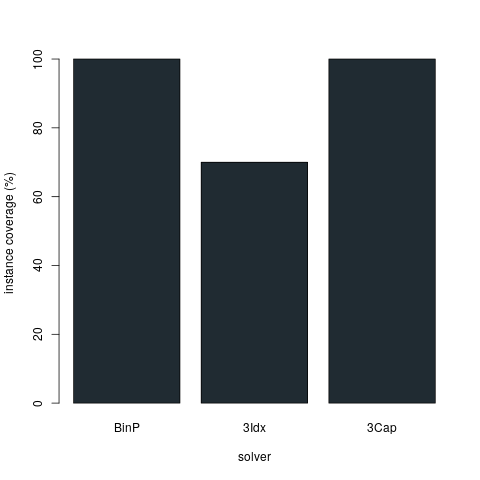
\includegraphics[width=1.2\textwidth]{img/solver_instance_coverage_b=3_m_600s.png}
\caption{\textsc{Zeitlimit} $10min$}
\label{fig:instance_coverage_b=3_m_a}
\end{subfigure}
\hfill
\begin{subfigure}[b]{0.3\textwidth}
\centering
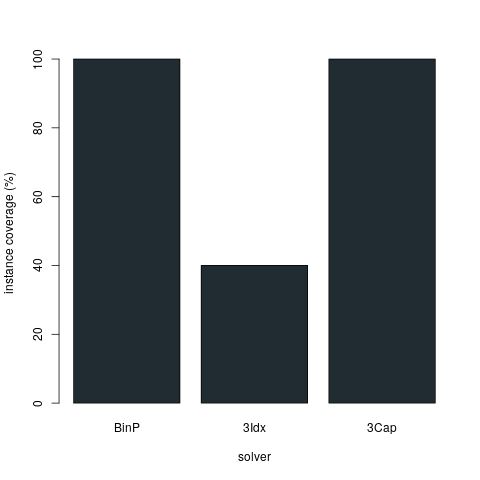
\includegraphics[width=1.2\textwidth]{img/solver_instance_coverage_b=3_m_1200s.png}
\caption{\textsc{Zeitlimit} $20min$}
\label{fig:instance_coverage_b=3_m_b}
\end{subfigure}
\hfill
\begin{subfigure}[b]{0.3\textwidth}
\centering
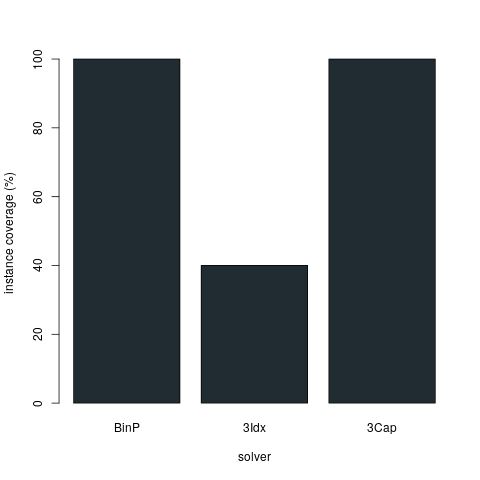
\includegraphics[width=1.2\textwidth]{img/solver_instance_coverage_b=3_m_1800s.png}
\caption{\textsc{Zeitlimit} $30min$}
\label{fig:instance_coverage_b=3_m_c}
\end{subfigure}
\caption{\textsc{Instance-Coverage}.}
\label{fig:instance_coverage_b=3_m}
\end{figure}

In Abb. \ref{fig:b=3_m_runtimes} ist zu sehen, dass sich die Laufzeiten der 3-Index-Formulierung bei jenen Instanzen,
welche von dieser gelöst werden, in der Regel nur marginal von denen der Bin-Packing-Formulierung unterscheiden,
wenngleich diese aufgrund der Instanzen $10$ und $13$ im Durchschnitt trotzdem um ca. $12 \%$ schneller ist.\newline
Die Heuristik ist, wie Abb. \ref{fig:b=3_m_runtimes} zu entnehmen, in Bezug auf die Laufzeit erneut konkurrenzlos.
Nach durchschnittlich $1.01s$ löst diese sämtliche Instanzen und unterbietet die MIP-Formulierungen damit um mehrere Größenordnungen.

Für die Kosten gilt, wie man Abb. \ref{fig:b=3_m_costs} entnehmen kann, dass die Ergebnisse der Heuristik,
wie in vorherigen Experimenten, eine Abweichung von den Optimalwerten der MIP-Formulierungen von durchschnittlich
unter einem Prozent besitzen. Beim dort betrachteten Zeitlimit von $10$ Minuten ermittelt die Heuristik mit den
Instanzen $00$ und $16$ in zwei Fällen sogar einen besseren Zielfunktionswert als die Bin-Packing-Formulierung,
obwohl diese dort auch zu zulässigen Lösungen gelangt.

\begin{figure}[H]
\centering
\begin{subfigure}[b]{0.4\textwidth}
\centering
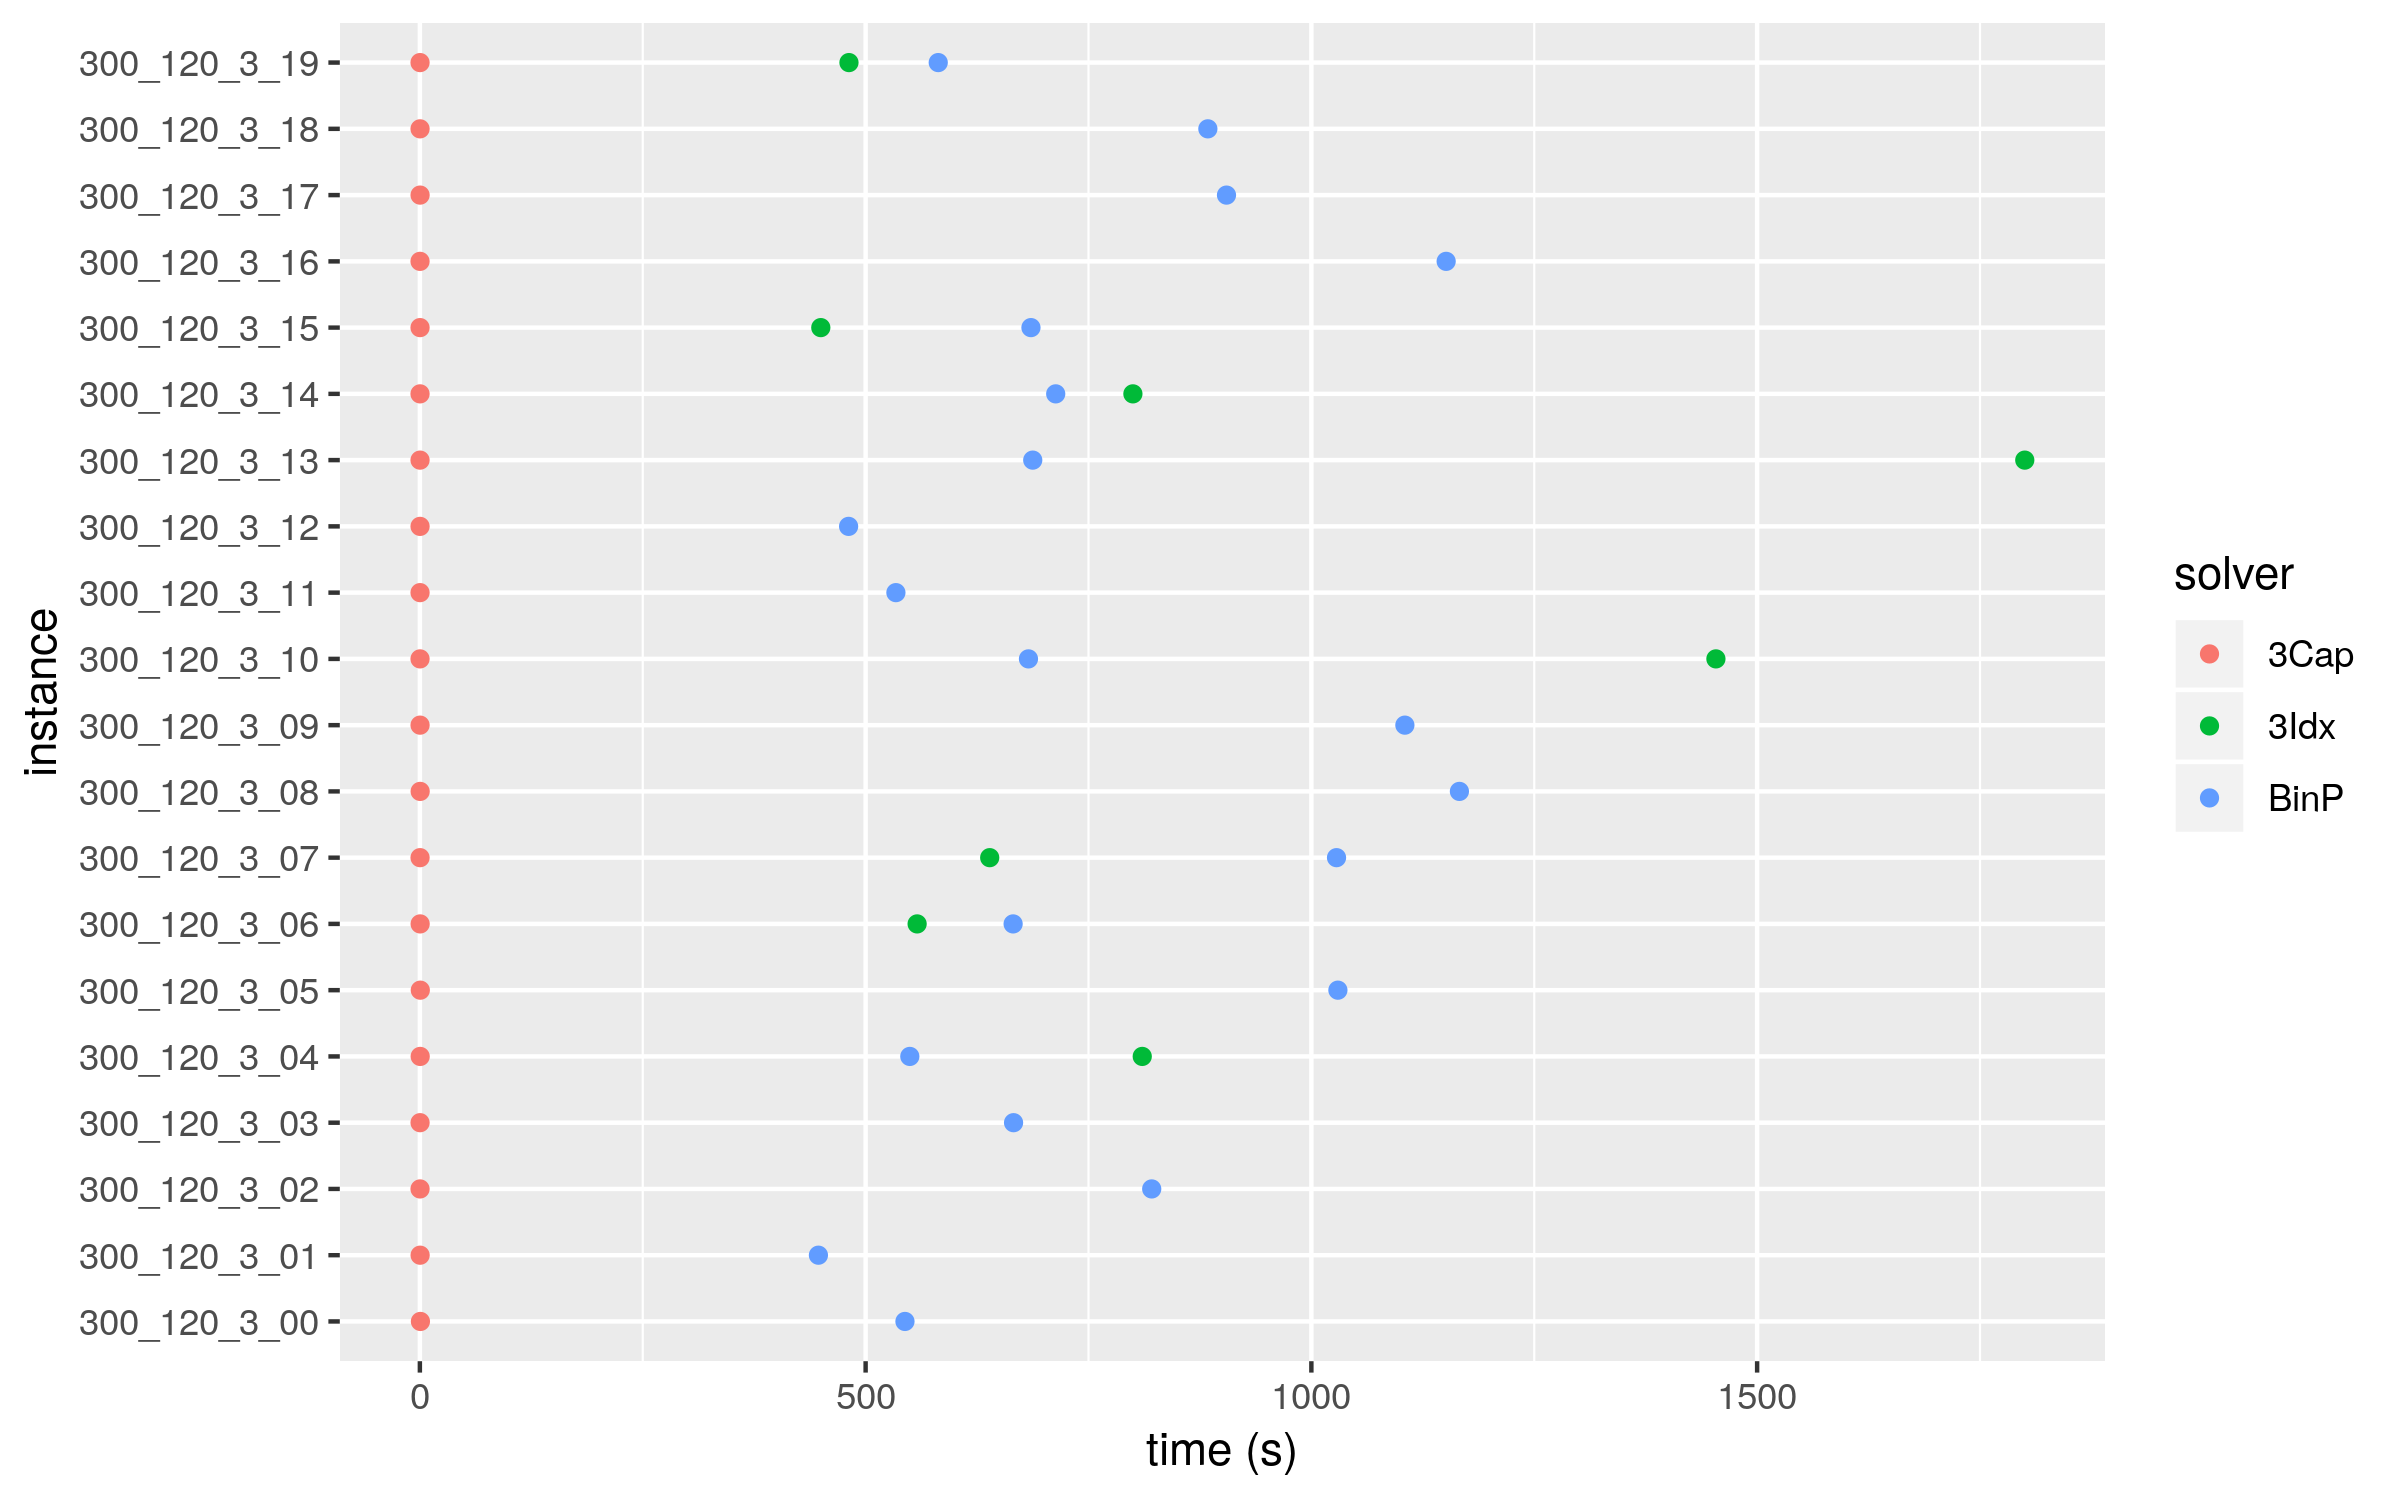
\includegraphics[width=1.3\textwidth]{img/solver_instance_time_b=3_m_1800s.png}
\caption{\textsc{Laufzeiten ($30min$ Zeitlimit)}}
\label{fig:b=3_m_runtimes}
\end{subfigure}
\hfill
\begin{subfigure}[b]{0.4\textwidth}
\centering
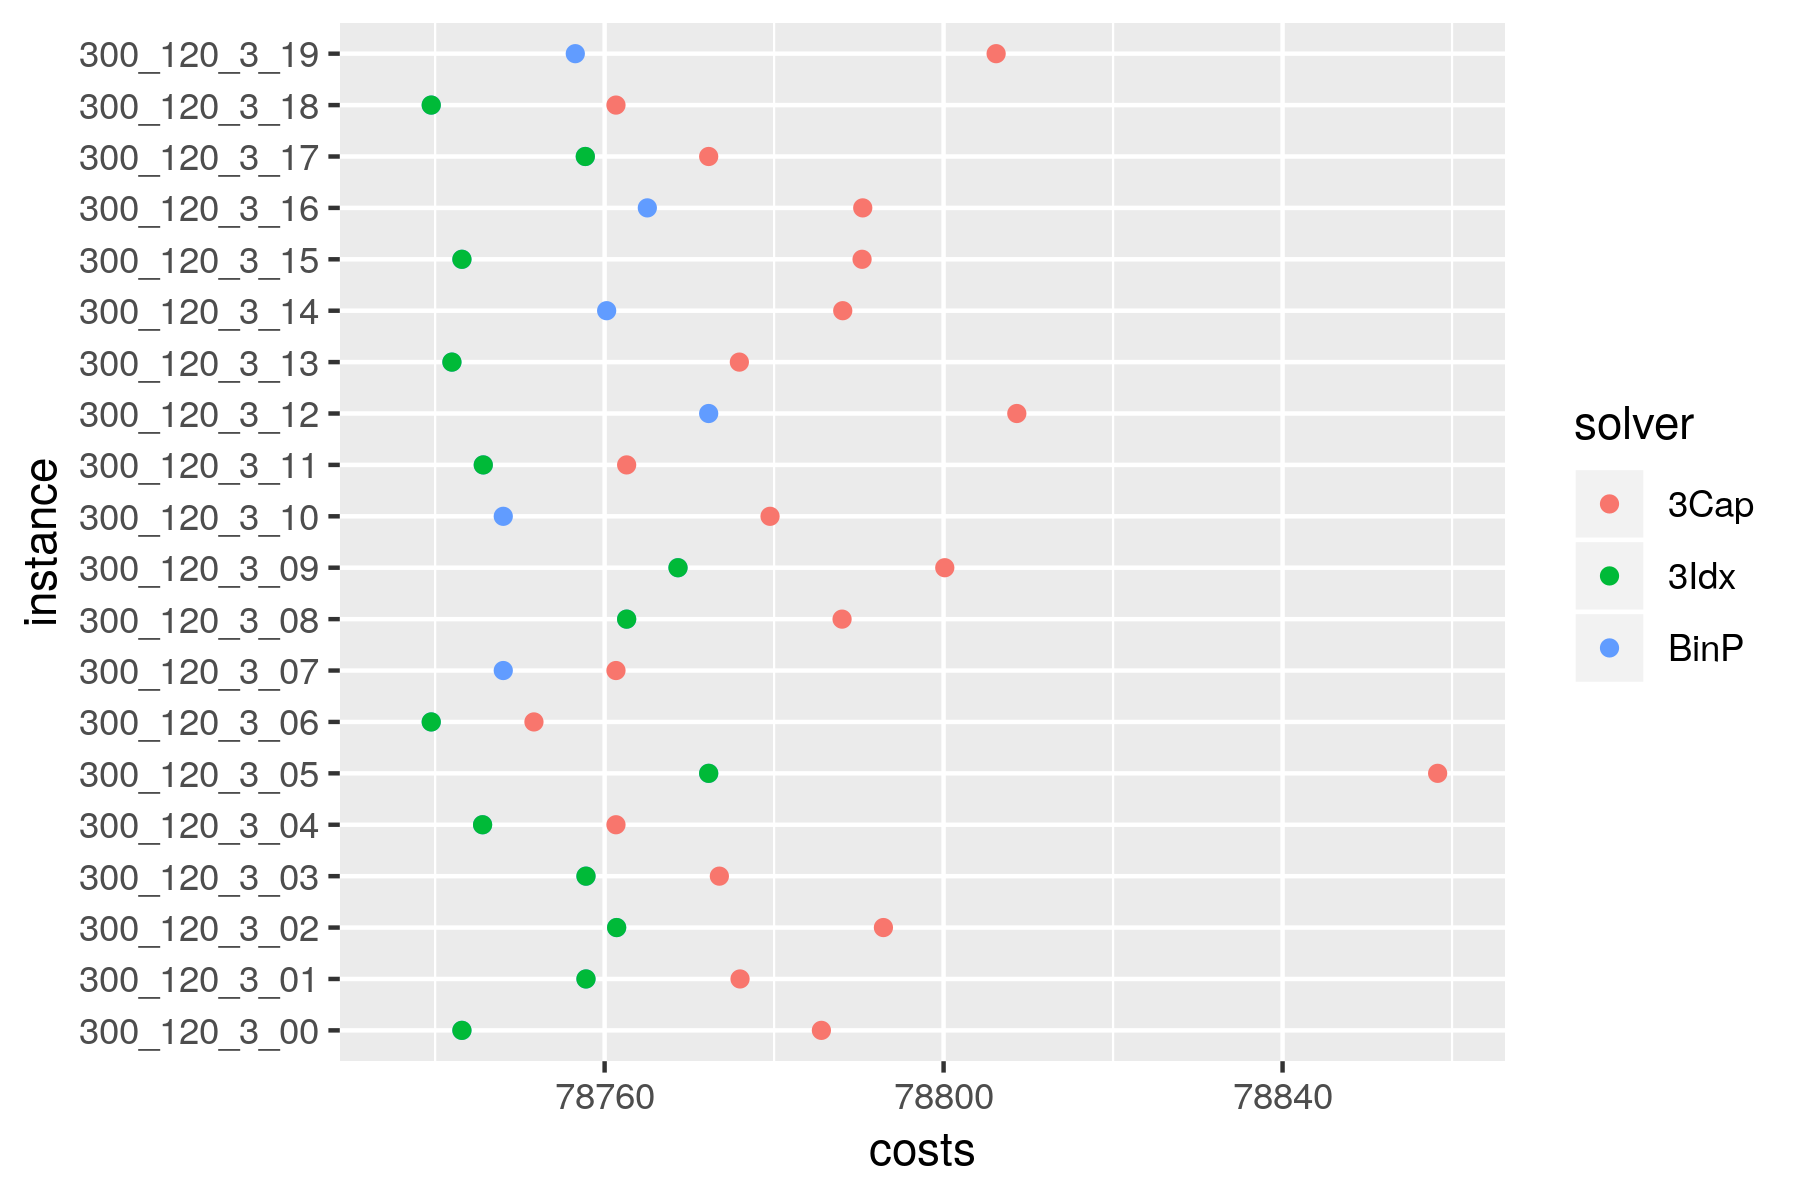
\includegraphics[width=1.3\textwidth]{img/solver_instance_cost_b=3_m_600s.png}
\caption{\textsc{Kosten ($10min$ Zeitlimit)}}
\label{fig:b=3_m_costs}
\end{subfigure}
\caption{\textsc{Ergebnisse}.}
\end{figure}

Abbildung \ref{fig:mip_results_b=3_m_a} bestätigt die Tendenz der Visualisierungen der Instance-Coverage und belegt,
dass beide MIP-Formulierungen bei einem Zeitlimit von $10$ Minuten nur wenige Instanzen überhaupt und noch weniger
Instanzen optimal lösen.
Bei einem Zeitlimit von $20$ Minuten hingegen, löst die Bin-Packing-Formulierung mit einer durchschnittlichen
Laufzeit von ca. $13$ Minuten pro Instanz sämtliche Instanzen optimal (vlg. Abb. \ref{fig:mip_results_b=3_m_b}).
Die 3-Index-Formulierung löst im Gegensatz dazu selbst bei einem Zeitlimit von $30$ Minuten nur $40 \%$ der Instanzen
optimal (vlg. Abb. \ref{fig:mip_results_b=3_m_c}), weshalb die Bin-Packing-Formulierung jener in dieser Kategorie erneut
klar vorzuziehen ist.

Die Heuristik benötigt durchschnittlich eine Laufzeit von nur $1.01s$ und weicht dabei um durchschnittlich
$0.35 \%$ vom Optimum ab. Wie bereits in der Kategorie der mittelgroßen Instanzen im $b = 2$ Szenario, ist dieser erhebliche
Laufzeitunterschied um mehrere Größenordnungen wohl hinreichende Motivation, um diese jeweils sehr geringe Abweichung
vom Optimum in Kauf zu nehmen.

\begin{figure}[H]
\begin{subfigure}[b]{0.3\textwidth}
\centering
\resizebox{\textwidth}{!}{
\begin{tabular}{ | l | l | l |}
    \hline
     & \textbf{BinP} & \textbf{3Idx} \\ \hline
    \textbf{Optimal} & $ \textcolor{mygreen}{50 \%}$ & $ \textcolor{red}{25 \%}$ \\ \hline
    \textbf{Laufzeit} & \O $\thinspace \textcolor{red}{583.7 s}$ & \O $\thinspace \textcolor{mygreen}{554.4 s}$ \\ \hline
    \textbf{Abweichung} & \O $\thinspace \textcolor{red}{0.2 \%}$ & \O $\thinspace \textcolor{mygreen}{0.01 \%}$ \\ \hline
\end{tabular}}
\caption{\textsc{Zeitlimit} $10min$}
\label{fig:mip_results_b=3_m_a}
\end{subfigure}
% $\quad\quad\quad\quad$
\begin{subfigure}[b]{0.3\textwidth}
\centering
\resizebox{\textwidth}{!}{
\begin{tabular}{ | l | l | l |}
    \hline
     & \textbf{BinP} & \textbf{3Idx} \\ \hline
    \textbf{Optimal} & $ \textcolor{mygreen}{100 \%}$ & $ \textcolor{red}{40 \%}$ \\ \hline
    \textbf{Laufzeit} & \O $\thinspace \textcolor{mygreen}{791.4 s}$ & \O $\thinspace \textcolor{red}{795.4 s}$ \\ \hline
    \textbf{Abweichung} & \O $\thinspace 0.0 \%$ & \O $\thinspace 0.0 \%$ \\ \hline
\end{tabular}}
\caption{\textsc{Zeitlimit} $20min$}
\label{fig:mip_results_b=3_m_b}
\end{subfigure}
% \end{figure}
% \begin{figure}[H]
\begin{subfigure}[b]{0.3\textwidth}
\centering
\resizebox{\textwidth}{!}{
\begin{tabular}{ | l | l | l |}
    \hline
     & \textbf{BinP} & \textbf{3Idx} \\ \hline
    \textbf{Optimal} & $ \textcolor{mygreen}{100 \%}$ & $ \textcolor{red}{40 \%}$ \\ \hline
    \textbf{Laufzeit} & \O $\thinspace \textcolor{mygreen}{766.4 s}$ & \O $\thinspace \textcolor{red}{874.0 s}$ \\ \hline
    \textbf{Abweichung} & \O $\thinspace 0.0 \%$ & \O $\thinspace 0.0 \%$ \\ \hline
\end{tabular}}
\caption{\textsc{Zeitlimit} $30min$}
\label{fig:mip_results_b=3_m_c}
\end{subfigure}

\caption{\textsc{MIP-Ergebnisse.}}
\label{fig:mip_results_b=3_m}
\end{figure}

\pagebreak

\textbf{Große Instanzen (l)}

Zuletzt werden die Solver für die in Kapitel \ref{sec:test_data} als groß bezeichneten Instanzen,
bei denen es darum geht, $500$ eintreffende Items in die Storage-Area zu verladen, verglichen.
In dieser Kategorie werden Zeitlimits von $45, 90$ und $120$ Minuten pro Instanz betrachtet.

Wie man Abb. \ref{fig:instance_coverage_b=3_l_a} entnehmen kann, findet keine der beiden MIP-Formulierungen
bei einem Zeitlimit von $45$ Minuten pro Instanz eine zulässige Lösung für eine der Instanzen.
Beim verdoppelten Zeitlimit von $90$ Minuten pro Instanz wird erkennbar, dass die Bin-Packing-Formulierung
mit einer Instance-Coverage von $80 \%$ auch in dieser Kategorie besser geeignet scheint, als die 3-Index-Formulierung,
welche selbst bei diesem Zeitlimit noch keine Instanz zulässig löst (vgl. \ref{fig:instance_coverage_b=3_l_b}).
Bei einem Zeitlimit von $120$ Minuten pro Instanz löst die Bin-Packing-Formulierung schließlich sämtliche Instanzen,
während die 3-Index-Formulierung sogar dort nur $20 \%$ der Instanzen löst (vgl. \ref{fig:instance_coverage_b=3_l_c}).

Die Heuristik ist mit einer durchschnittlichen Laufzeit von $3.9s$ pro Instanz erneut in keinem Fall
vom Zeitlimit betroffen.

\begin{figure}[H]
\centering

\begin{subfigure}[b]{0.3\textwidth}
\centering
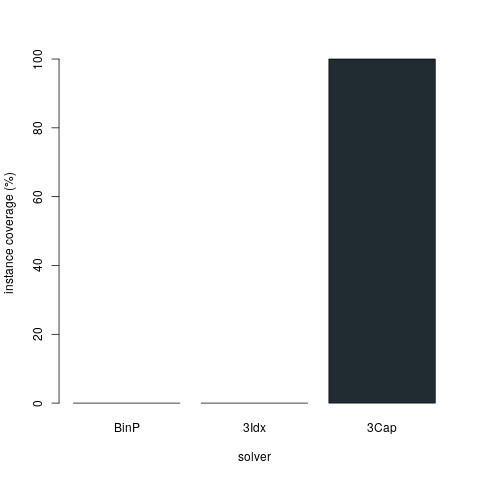
\includegraphics[width=1.2\textwidth]{img/solver_instance_coverage_b=3_l_2700s.png}
\caption{\textsc{Zeitlimit} $45min$}
\label{fig:instance_coverage_b=3_l_a}
\end{subfigure}
\hfill
\begin{subfigure}[b]{0.3\textwidth}
\centering
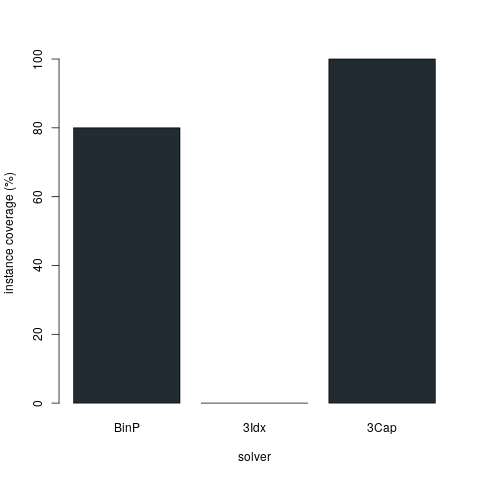
\includegraphics[width=1.2\textwidth]{img/solver_instance_coverage_b=3_l_5400s.png}
\caption{\textsc{Zeitlimit} $90min$}
\label{fig:instance_coverage_b=3_l_b}
\end{subfigure}
\hfill
\begin{subfigure}[b]{0.3\textwidth}
\centering
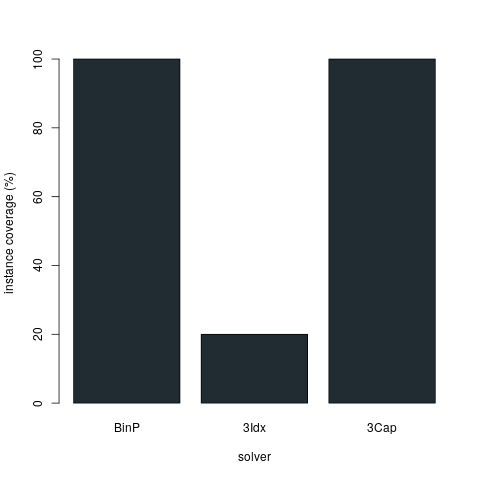
\includegraphics[width=1.2\textwidth]{img/solver_instance_coverage_b=3_l_7200s.png}
\caption{\textsc{Zeitlimit} $120min$}
\label{fig:instance_coverage_b=3_l_c}
\end{subfigure}
\caption{\textsc{Instance-Coverage}.}
\label{}
\end{figure}

Wie man Abb. \ref{fig:b=3_l_runtimes} entnehmen kann, ist die Bin-Packing-Formulierung in den wenigen
Fällen, in welchen die 3-Index-Formulierung zu einer zulässigen Lösung gelangt, stets schneller
als diese. Des Weiteren erkennt man, dass die Heuristik wie erwartet auch hier konkurrenzlos ist.

In Abb. \ref{fig:b=3_l_costs} ist zu erkennen, dass die Heuristik in einem der drei Fälle, in welchen die
3-Index-Formulierung zu einer zulässigen Lösung gelangt, einen besseren Zielfunktionswert als diese erzielt.
Außerdem ist zu sehen, dass die Abweichungen der Zielfunktionswerte der Heuristik von denen der Bin-Packing-Formulierung
erneut nur sehr gering sind.

\begin{figure}[H]
\centering
\begin{subfigure}[b]{0.4\textwidth}
\centering
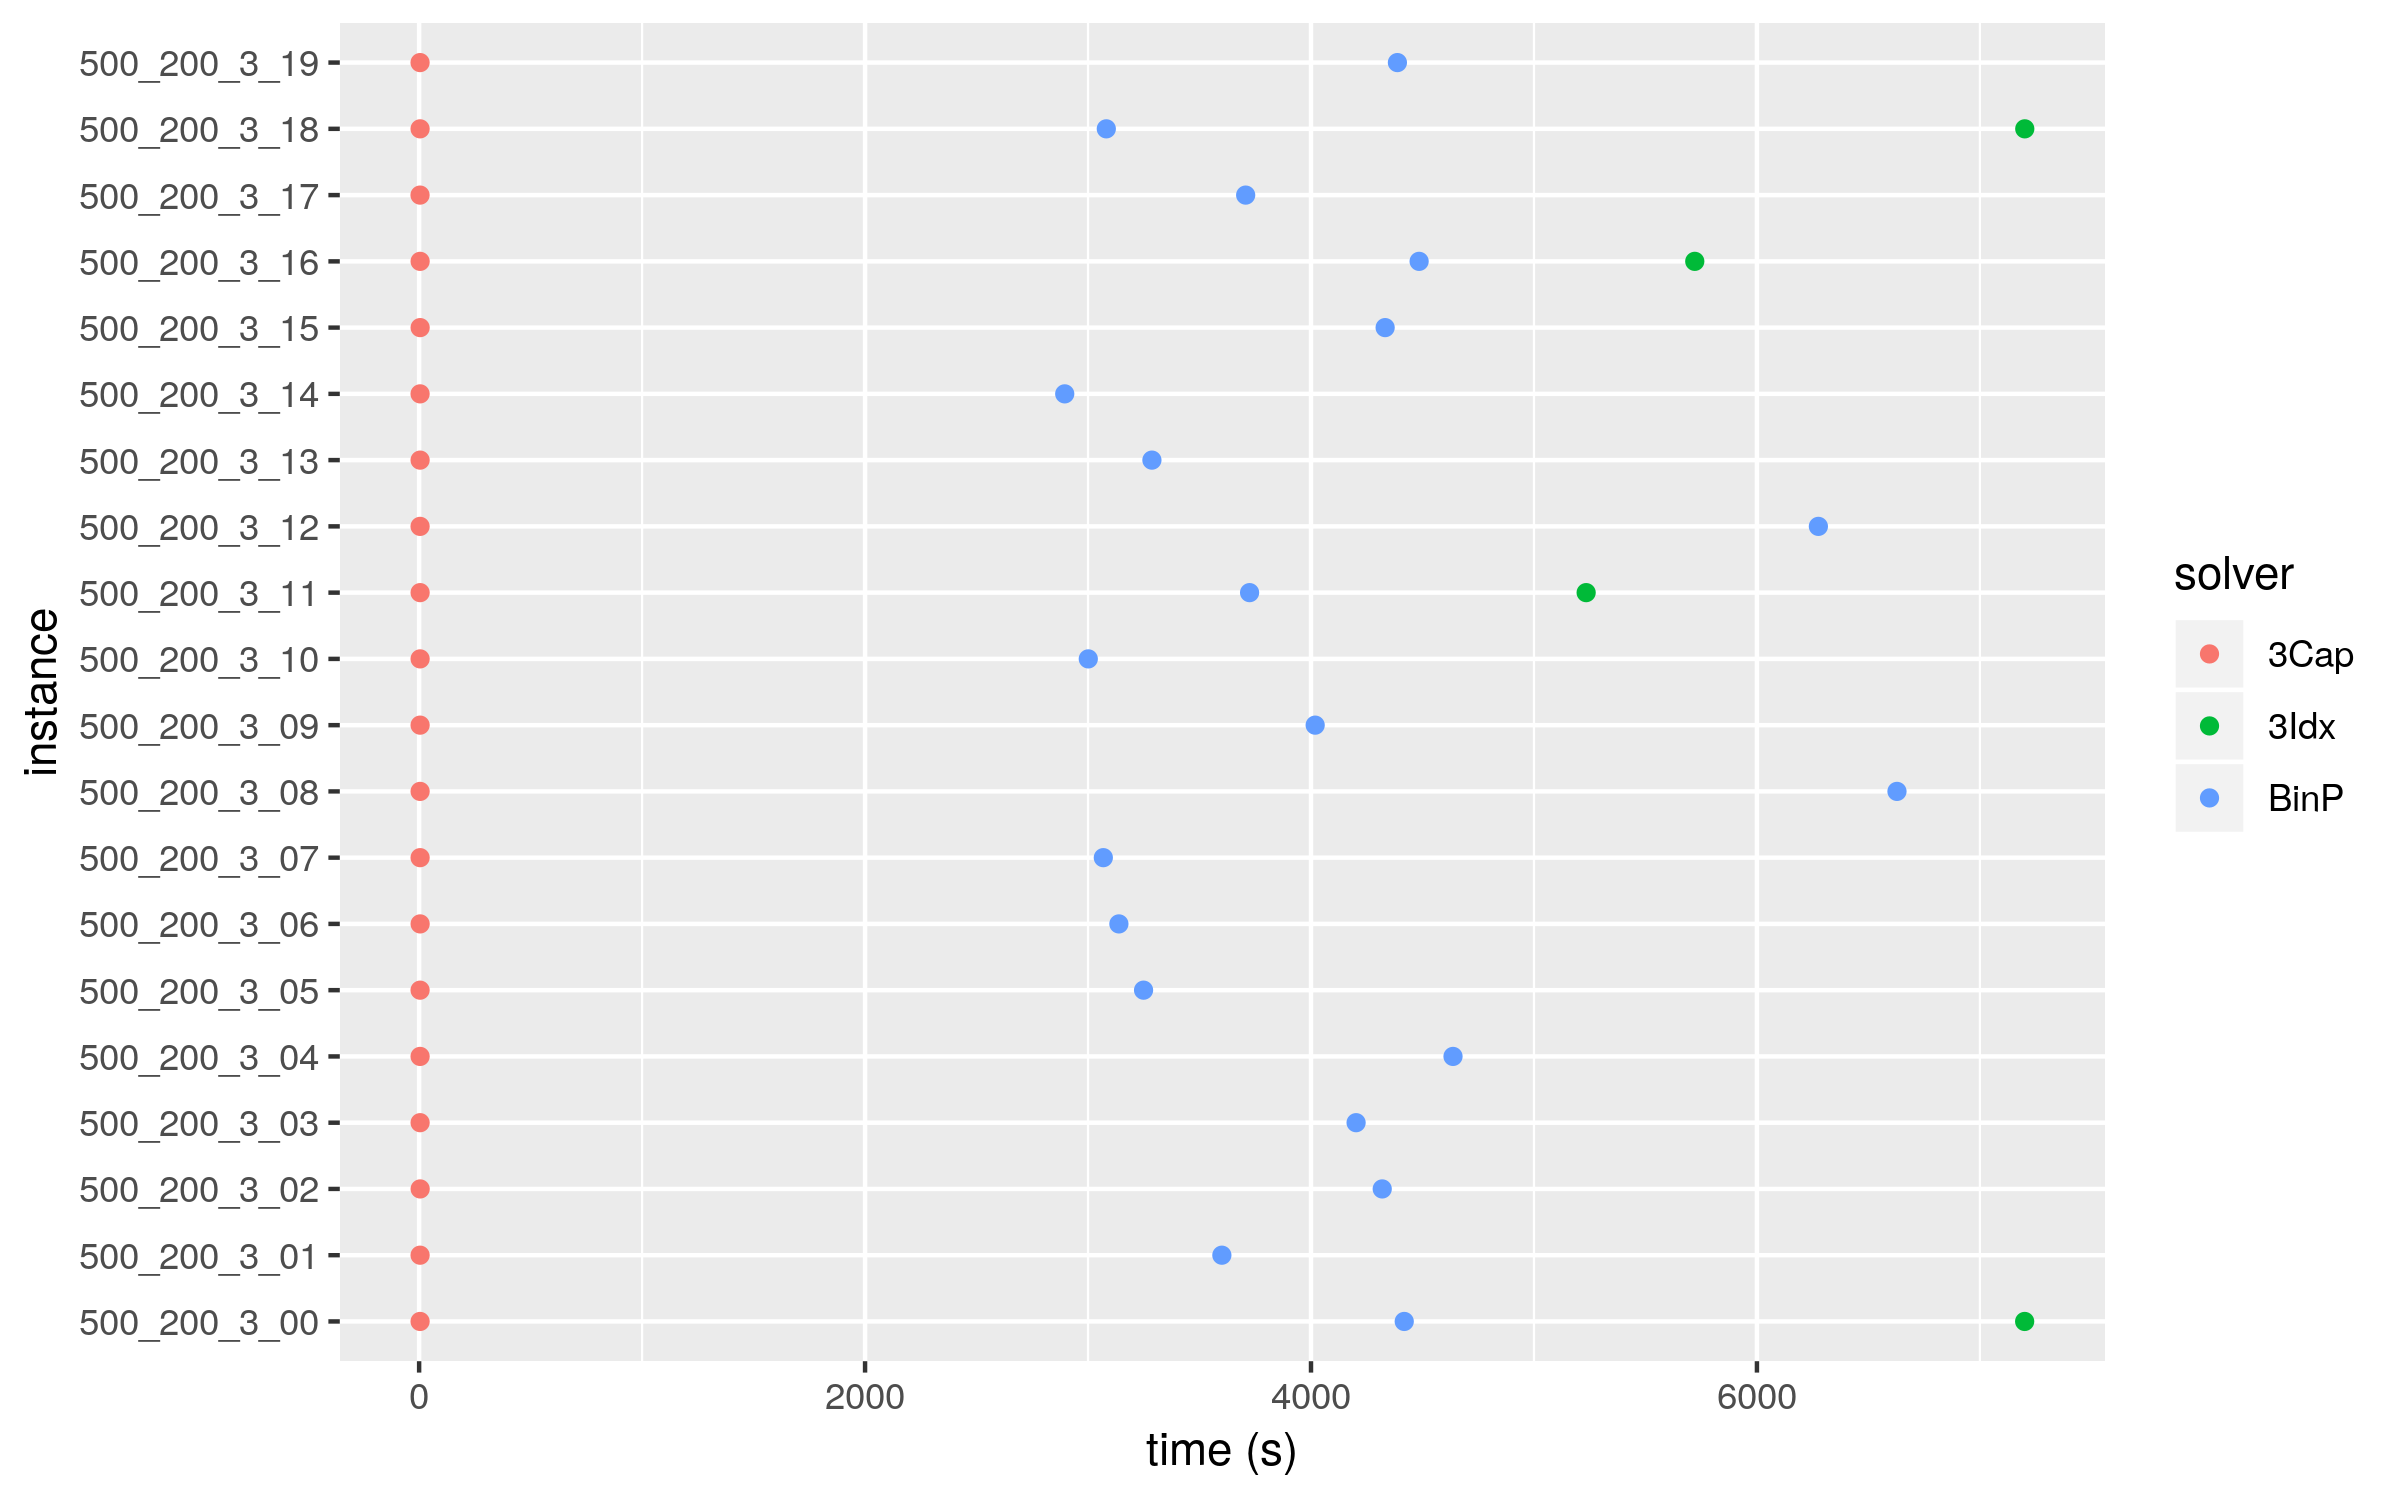
\includegraphics[width=1.3\textwidth]{img/solver_instance_time_b=3_l_7200s.png}
\caption{\textsc{Laufzeiten}}
\label{fig:b=3_l_runtimes}
\end{subfigure}
\hfill
\begin{subfigure}[b]{0.4\textwidth}
\centering
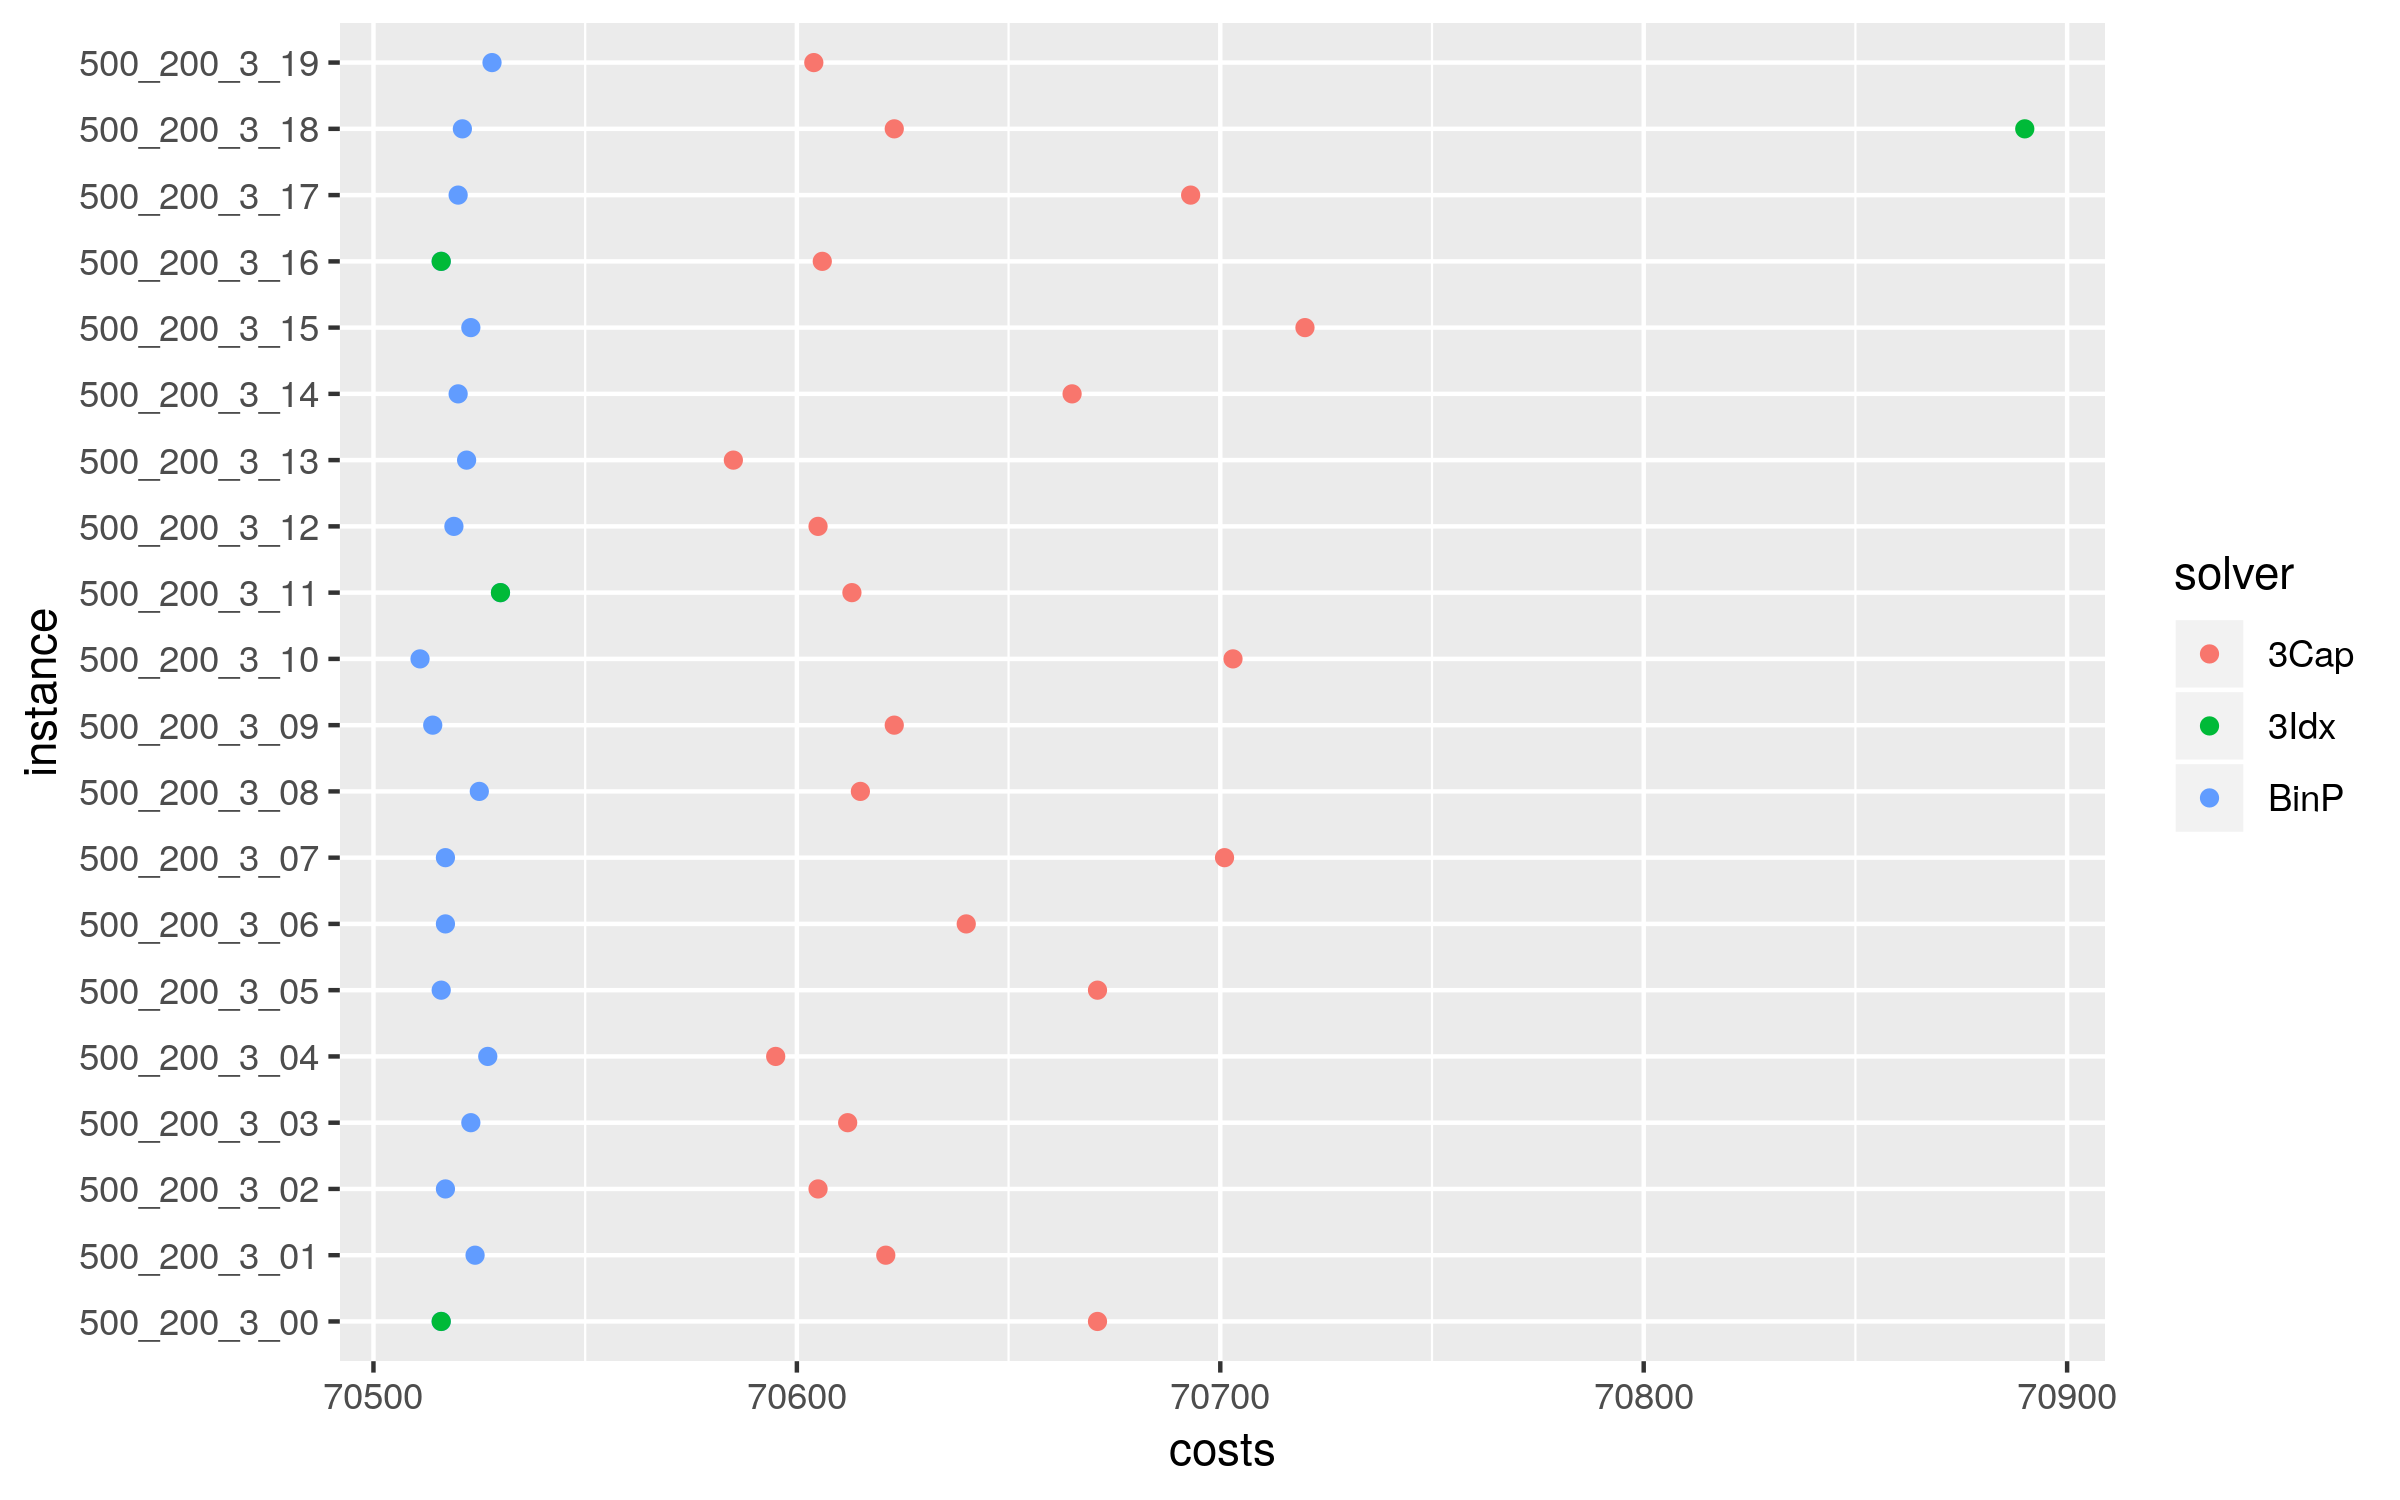
\includegraphics[width=1.3\textwidth]{img/solver_instance_cost_b=3_l_7200s.png}
\caption{\textsc{Kosten}}
\label{fig:b=3_l_costs}
\end{subfigure}
\caption{\textsc{Ergebnisse bei $120min$ Zeitlimit}.}
\label{fig:res_plots_b=3_l}
\end{figure}

Wie bereits erwähnt, ist die 3-Index-Formulierung in dieser Kategorie erneut der Bin-Packing-Formulierung
unterlegen, welche, wie man in Abb. \ref{fig:mip_results_b=3_l_c} erkennt, nach durchschnittlich
etwas mehr als einer Stunde sämtliche Instanzen optimal löst.

% TODO: ggf. später noch einmal durchführen
Die Verringerung der durchschnittlichen Laufzeit der Bin-Packing-Formulierung zwischen den betrachteten
Zeitlimits von $90$ und $120$ Minuten um mehrere Minuten ist überraschend und lässt sich vermutlich
lediglich durch unterschiedliche Auslastungen des Systems, auf welchem die Experimente durchgeführt wurden,
zu unterschiedlichen Zeiten erklären.

\begin{figure}[H]
\begin{subfigure}[b]{0.3\textwidth}
\centering
\resizebox{\textwidth}{!}{
\begin{tabular}{ | l | l | l |}
    \hline
     & \textbf{BinP} & \textbf{3Idx} \\ \hline
    \textbf{Optimal} & $ 0 \%$ & $ 0 \%$ \\ \hline
    \textbf{Laufzeit} & $---$ & $---$ \\ \hline
    \textbf{Abweichung} & $---$ & $---$ \\ \hline
\end{tabular}}
\caption{\textsc{Zeitlimit} $45min$}
\label{fig:mip_results_b=3_l_a}
\end{subfigure}
% $\quad\quad\quad\quad$
\begin{subfigure}[b]{0.3\textwidth}
\centering
\resizebox{\textwidth}{!}{
\begin{tabular}{ | l | l | l |}
    \hline
     & \textbf{BinP} & \textbf{3Idx} \\ \hline
    \textbf{Optimal} & $ \textcolor{mygreen}{80 \%}$ & $ \textcolor{red}{0 \%}$ \\ \hline
    \textbf{Laufzeit} & $\textcolor{mygreen}{4511.5}$ & $\textcolor{red}{---}$ \\ \hline
    \textbf{Abweichung} & $\textcolor{mygreen}{0 \%}$ &$\textcolor{red}{---}$ \\ \hline
\end{tabular}}
\caption{\textsc{Zeitlimit} $90min$}
\label{fig:mip_results_b=3_l_b}
\end{subfigure}
% \end{figure}
% \begin{figure}[H]
\begin{subfigure}[b]{0.3\textwidth}
\centering
\resizebox{\textwidth}{!}{
\begin{tabular}{ | l | l | l |}
    \hline
     & \textbf{BinP} & \textbf{3Idx} \\ \hline
    \textbf{Optimal} & $ \textcolor{mygreen}{100 \%}$ & $ \textcolor{red}{15 \%}$ \\ \hline
    \textbf{Laufzeit} & $\textcolor{mygreen}{4022.9}$ & $\textcolor{red}{6339.3}$ \\ \hline
    \textbf{Abweichung} & $\textcolor{mygreen}{0 \%}$ &$\textcolor{red}{0.13 \%}$ \\ \hline
\end{tabular}}
\caption{\textsc{Zeitlimit} $120min$}
\label{fig:mip_results_b=3_l_c}
\end{subfigure}
\caption{\textsc{MIP-Ergebnisse.}}
\label{}
\end{figure}

Die Heuristik löst mit einer durchschnittlichen Laufzeit von $3.9s$ pro Instanz sämtliche Instanzen
und weicht dabei im Durchschnitt nur um $0.17 \%$ vom Optimum ab.

\textbf{Fazit}\newline

Bei Stacking-Problemen mit Stacks der Kapazität $b = 3$ besteht in der Kategorie der kleinen Instanzen
aufgrund der relativ geringen Laufzeit der Bin-Packing-Formulierung nicht zwingend ein Bedarf für eine
Laufzeitverbesserung durch eine Heuristik. Nichtsdestotrotz ist die Heuristik bei einer nur geringen
durchschnittlichen Abweichung vom Optimum noch einmal erheblich schneller als diese.

In der Kategorie der mittelgroßen Instanzen ist die Bin-Packing-Formulierung der 3-Index-Formulierung sogar
sehr deutlich vorzuziehen. Da jedoch auch die Bin-Packing-Formulierung durschnittlich $13$ Minuten zur exakten Lösung benötigt,
ermöglicht die Heuristik hier mit einer durchschnittlichen Laufzeit von nur ca. einer Sekunde eine derart große Laufzeitersparnis,
dass die sehr geringe Abweichung von $0.35 \%$ in Kauf genommen werden sollte.

Noch deutlicher äußert sich dieser Trend in der Kategorie der großen Instanzen, in welcher die 3-Index-Formulierung
selbst bei einem Zeitlimit von zwei Stunden nur $20 \%$ der Instanzen löst. Die Bin-Packing-Formulierung, welche dort
mit einer durchschnittlichen Laufzeit von etwas mehr als einer Stunde sämtliche Instanzen optimal löst,
ist demnach bei einer Stack-Kapazität von $b = 3$ in jeder Kategorie der 3-Index-Formulierung vorzuziehen.
Die Heuristik benötigt hier durschnittlich $3.9s$ pro Instanz und weicht um durchschnittlich $0.17 \%$ vom Optimum ab.
Der daraus resultierende noch gravierendere Unterschied der Laufzeiten zwischen der Bin-Packing-Formulierung und
der Heuristik sorgt in Verbindung mit der sehr geringen Abweichung vom Optimum dafür, dass die Heuristik in der Praxis
auch in dieser Kategorie bevorzugt werden sollte.

Insgesamt ist festzuhalten, dass die Heuristik in jeder betrachteten Kategorie bei sehr geringen Abweichungen
vom Optimum deutlich kürzere Laufzeiten als die von \textsc{CPLEX} gelösten MIP-Formulierungen bietet und somit in
jedem Fall eine gute Alternative darstellt. Je größer die Instanzen werden, desto besser schneidet die Heuristik
verglichen mit den MIP-Formulierungen ab und sollte bereits ab der Kategorie der mittelgroßen Instanzen in der Regel
den MIP-Formulierungen vorgezogen werden.

% TODO: insert observation

An jener Stelle in der Heuristik, an welcher das Rating-System zum Einsatz kommt, um unterschiedlich sortierte
Listen der Item-Paare zu bilden, hätten zusätzlich zufällige \textquote{Shuffles} genutzt werden können,
um weitere Permutationen zu generieren. Besonders bei einer hohen Anzahl solcher Shuffles,
kann dabei mitunter ein besserer Zielfunktionswert erzielt werden. Dieser Ansatz wird jedoch aus zwei Gründen in
dieser Arbeit nicht verfolgt. Zunächst ist eine verhältnismäßig große Anzahl solcher Shuffles vonnöten um in
manchen Fällen zu bessren Ergebnissen zu gelangen, was eine erhebliche Verlängerung der Laufzeit zur Folge hätte.
Des Weiteren führt ein solcher stochastischer Ansatz dazu, dass für eine Instanz nicht mehr stets dasselbe Ergebnis
generiert wird. Da es sich bei den auf diese Weise erreichbaren Verbesserungen jedoch in der Regel nur um minimale
Verbesserungen handelt, die zum Preis einer extrem erhöhten Laufzeit kommen, wird dies nicht in Kauf genommen.
Stattdessen handelt es sich bei der präsentierten Heuristik, wie auch bei der Heuristik für $b = 2$ aus Abschnitt
\ref{sec:two_cap_heuristic}, um ein deterministisches Verfahren, welches bei denselben Rahmenbedingungen für eine Instanz
stets zum selben Ergebnis kommt.

\section{Verbesserungsverfahren}
\label{sec:post_optimization}

Bei Verbesserungsverfahren handelt es sich um lokale Suchverfahren, welche bereits mit einer Lösung des Problems starten,
die z.B. durch ein konstruktives Eröffnungsverfahren, wie die Heuristiken aus den Kapiteln \ref{sec:two_cap_heuristic} und \ref{sec:three_cap_heuristic} bestimmt wurden und versuchen diese im Laufe des Verfahrens zu verbessern.

Dabei wird zwischen deterministischen Verfahren, die bei gleichen Startlösungen und gleichen Rahmenbedingungen stets zum gleichen
Ergebnis kommen und stochastischen Verfahren, bei denen durch den Einsatz einer Zufallskomponente unterschiedliche Lösungen
generiert werden, unterschieden. \cite{Knust2017}

\subsection{Lokale Suchverfahren}
\label{sec:local_search}

Bei den in dieser Arbeit betrachteten lokalen Suchverfahren handelt es sich um sogenannte Metaheuristiken,
weil sie nicht auf ein spezielles Problem abzielen, sondern auf grundsätzlichen Suchprinzipien beruhen,
die auf eine Vielzahl von Optimierungsproblemen anwendbar sind.
Aus diesem Grund erfreuen sich diese Heuristiken einer sehr großen Beliebtheit,
sie sind allgemein anwendbar und sehr flexibel an konkrete Problemstellungen anpassbar.

Eine lokale Suche ist ein iterativer Prozess, bei welchem von einer Lösung zur nächsten, verbessernden Lösung vorangeschritten wird,
bis ein bestimmtes Abbruchkriterium erfüllt ist. Um den Lösungsraum systematisch zu durchsuchen, wird die
sogenannte Nachbarschaft einer Lösung definiert, die der Menge der Lösungen entspricht, die im nächsten Schritt
von der gegenwärtigen Lösung erreichbar sind. \cite{Brucker2006}

Die Idee eines lokalen Suchverfahrens ist es also, ausgehend von einer Initiallösung, durch wohldefinierte Regeln zu anderen,
verbessernden Lösungen innerhalb der Nachbarschaft zu gelangen.
Dabei wird häufig solange fortgeschritten, bis keine verbessernde Lösung in der Nachbarschaft gefunden wird,
also bis ein lokales Minimum erreicht ist.

Der Erfolg dieses Ansatzes und somit die Lösungsqualität hängt primär von der definierten Struktur der Nachbarschaft ab. \cite{Pirlot1996}

Die größte Schwäche dieses Ansatzes ist die Unfähigkeit, lokale Minima zu verlassen. Dieses Problem ist sehr
anschaulich in Abb. \ref{fig:local_search_weakness} visualisiert. Darin sind sämtliche Lösungen in der Nachbarschaft $V(x_n)$ schlechter
als die gegenwärtige Lösung $x_n$, obwohl weiter entfernt ein globales Minimum existiert, welches
aufgrund der Tatsache, dass ausschließlich verbessernde Lösungen gewählt werden, nicht erreicht werden kann.

\begin{figure}[H]
\centering
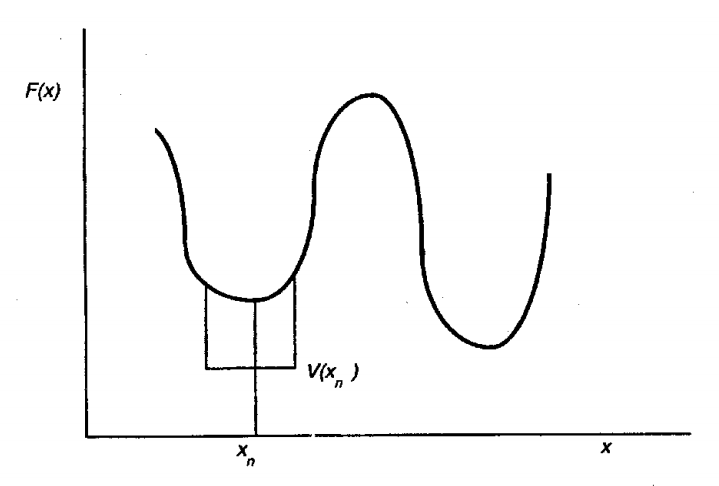
\includegraphics[width=0.6\textwidth]{img/local_minimum.png}
\caption{\textsc{Schwäche lokaler Suchverfahren. \cite{Pirlot1996}}}
\label{fig:local_search_weakness}
\end{figure}

\textbf{Formaler Ablauf einer lokalen Suche}

Eine lokale Suche startet mit einer beliebigen Lösung $x_1 \in X$ und in jedem Schritt $n$
wird eine neue Lösung $x_{n+1}$ aus der Nachbarschaft $V(x_n)$ der gegenwärtigen Lösung $x_n$ gewählt.
Für jedes $x \in X$ existiert eine solche Nachbarschaft $V(x) \subseteq X$.
Typischerweise entspricht das Kriterium, anhand welchem die nächste Lösung $x_{n+1}$ gewählt wird,
die beste Lösung in der Nachbarschaft von $x_n$ zu wählen, also eine Lösung $x_{n+1} \in V(x_n)$
mit $F(x_{n+1}) \leq F(x) \forall x \in V(x_n)$. \cite{Pirlot1996}

Sollte keine verbessernde Lösung in der Nachbarschaft gefunden werden, so terminiert die Suche.
Diese Strategien wird \textquote{Steepest Descent} genannt, also Strategie des steilsten Abstiegs.
Dieser Name ergibt sich daraus, dass bei einem Minimierungsproblem in der Richtung des steilsten Abstiegs
von der Initiallösung vorangeschritten wird, bis keine Verbesserung mehr erzielt wird. Diese Strategie führt zum
bereits erwähnten Problem aus Abb. \ref{fig:local_search_weakness}.

\textbf{Beispiel}

Ein simples Beispiel für eine solche Nachbarschaft ist ein Bitvektor. Wenn $X$ eine Menge
von Bitvektoren ist und $x \in X$, dann kann eine Nachbarschaft $V(x)$ als die Menge
sämtlicher Lösungen $x \in X$ definiert werden, bei denen in $x$ ein einzelnes Bit invertiert wird. \cite{Pirlot1996}

Sei $x = \{1, 1, 1, 0, 1, 0\}$ eine als Bitvektor kodierte Lösung.
Die Nachbarschaft dieser Lösung sieht nun gemäß der beschrieben Struktur wie folgt aus:
\[
V(x) =
  \begin{bmatrix}
    \boldsymbol{0} & 1 & 1 & 0 & 1 & 0 \\
    1 & \boldsymbol{0} & 1 & 0 & 1 & 0 \\
    1 & 1 & \boldsymbol{0} & 0 & 1 & 0 \\
    1 & 1 & 1 & \boldsymbol{1} & 1 & 0 \\
    1 & 1 & 1 & 0 & \boldsymbol{0} & 0 \\
    1 & 1 & 1 & 0 & 1 & \boldsymbol{1}
  \end{bmatrix}
\]

\pagebreak

\subsection{Tabu-Suche}
\label{sec:tabu_seach}

Das größte Problem des in Kapitel \ref{sec:local_search} vorgestellten allgemeinen lokalen Suchverfahrens
ist, dass die Lösung nur einem lokalen Minimum entspricht und daher möglicherweise stark vom globalen
Minimum abweicht. Eine gute Qualität der Lösung ist somit nicht garantiert.

Eine Strategie um diesem Problem entgegenzutreten wäre beispielsweise, das Verfahren mehrfach mit unterschiedlichen
Initiallösungen zu starten und anschließend das beste generierte lokale Minimum zu wählen.
Ein weiterer Ansatz ist, Verschlechterungen des Zielfunktionswerts während des Suchprozesses zu erlauben.
Das führt allerdings dazu, dass Lösungen mehrfach besucht werden können und somit Zyklen entstehen können.
Somit müssen in solchen Ansätzen zusätzliche Strategien umgesetzt werden, die Zyklen vermeiden. \cite{Brucker2006}

Genau dort setzt das Verfahren der sogenannten Tabu-Suche an. Eine Tabu-Suche besitzt eine Tabu-Liste,
in der sämtliche Lösungen, die besucht werden, als zukünftig \textquote{tabu} gespeichert werden.
Eine zur gegenwärtigen Lösung benachbarte Lösung wird nur dann akzeptiert, wenn diese nicht Teil der Tabu-Liste ist.
In jeder Iteration wird die gegenwärtige Lösung demnach durch eine benachbarte Lösung ersetzt, die nicht \textquote{tabu} ist.

\begin{figure}[H]
\centering
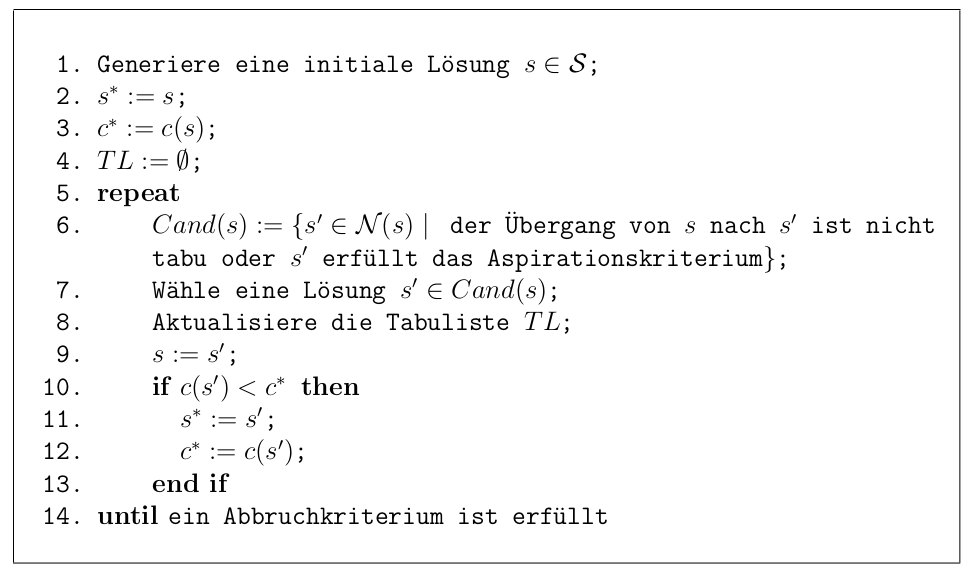
\includegraphics[width=0.9\textwidth]{img/tabu_search_algo_placeholder.png}
\caption{\textsc{Tabu-Suche. \cite{Knust2017}}}
\label{fig:local_search_weakness}
\end{figure}

\pagebreak

\section{Fazit}
\label{sec:conclusion}

% TODO: to be elaborated
Die MIP-Formulierungen könnten auch deshalb noch etwas bessere Zielfunktionswerte liefern, weil
diese ausschließlich die Kosten minimieren.
Die Heuristiken betrachten, wie in Kapitel \ref{sec:stacking_problems} erläutert, eine Kombination zweier Zielfunktionen
und gehen dementsprechend über einen reinen Fokus auf Kostenminimierung hinaus.
